\documentclass{mcmthesis}
\mcmsetup{CTeX = false,
        tcn = 19678, problem = B,
        sheet = true, titleinsheet = false, keywordsinsheet = false,
        titlepage = false, abstract = false}
\setlength{\headheight}{13.6pt}
\usepackage{bookman}
%\usepackage{times}
%to get dummy loremipsum text
\usepackage{lipsum}
\usepackage{subcaption}
\usepackage{booktabs}
\usepackage[table]{xcolor}
\usepackage{longtable}
\usepackage{amsmath}
\usepackage{mathtools}
\usepackage{blkarray}
\usepackage{caption}
\usepackage{nicematrix}
\usepackage{xltabular}
\usepackage{tabularx}
\usepackage{graphicx}
\usepackage{float}
\usepackage{lmodern}
\usepackage{algorithm2e}
\usepackage{titlesec}
\RestyleAlgo{ruled}
\usepackage{indentfirst}
\usepackage{pdfpages}
% \usepackage{newpxtext,newpxmath}
\usepackage[numbib,nottoc]{tocbibind}
\usepackage[svgnames]{xcolor}
\usepackage{multicol}
\usepackage[none]{hyphenat}
\usepackage{xurl}
% Allow citation-bearing lines to wrap within the existing margins.
\setlength{\emergencystretch}{3em}
\usepackage{ragged2e}
\usepackage{comment}
\usepackage[export]{adjustbox}
\usepackage{needspace}
\lstdefinestyle{Rcode}{
    basicstyle=\ttfamily\scriptsize,
    breaklines=true,
    columns=fullflexible,
    showstringspaces=false
}
\DeclareUnicodeCharacter{03BB}{\ensuremath{\lambda}}
\DeclareUnicodeCharacter{03BC}{\ensuremath{\mu}}
\DeclareUnicodeCharacter{03C3}{\ensuremath{\sigma}}
\DeclareUnicodeCharacter{2248}{\ensuremath{\approx}}
\DeclareUnicodeCharacter{00B2}{\ensuremath{^2}}
\DeclareUnicodeCharacter{00B7}{\ensuremath{\cdot}}
\DeclareUnicodeCharacter{2013}{--}
\DeclareUnicodeCharacter{2212}{\ensuremath{-}}
\DeclareUnicodeCharacter{00D7}{\ensuremath{\times}}
\DeclareUnicodeCharacter{03B8}{\ensuremath{\theta}}
\DeclareUnicodeCharacter{2080}{\ensuremath{_0}}
\DeclareUnicodeCharacter{2081}{\ensuremath{_1}}


% %%% BIB SPACING
\newlength{\bibitemsep}
\newlength{\bibparskip}
\usepackage{bibspacing}
\setlength{\bibitemsep}{.2\baselineskip plus .05\baselineskip minus .05\baselineskip}

% %for unknown reason, including the following packa4ges changes the style of the contents section
% \usepackage{multicol}
% \usepackage{tocloft}
% \usepackage{titletoc}
\title{HiMCM}

%% Assumption Table Numbering
\newcolumntype{Y}{>{\raggedright\arraybackslash}X}
\newcounter{assumption}
\newcommand{\nextassumption}{\refstepcounter{assumption}\arabic{assumption}}
%%%%%%%%%%%%%%%%%%

%%%% CHANGE MARGINS COMMAND %%%%%

\def\changemargin#1#2{\list{}{\rightmargin#2\leftmargin#1}\item[]}
\let\endchangemargin=\endlist 

%%%%%%%%%%


%% TITLE PAGE. SUMMARY PAGE FORMATTING
\titleformat{\section}[block]
{\fontfamily{cmr}\centering\large\scshape\bfseries}{\thesection}{1em}{}
\titlespacing*{\section}
{0pt}{2.5ex plus 1ex minus .2ex}{2.5ex plus .2ex}
\date{\today}
\begin{document}
\begin{abstract}

%%%% SUMMARY PAGE %%%%%
\begin{center}
{\fontfamily{cmr}\large\scshape\bfseries Summary}
\end{center}
\begin{changemargin}{0.15in}{0.15in} 
\noindent\hspace*{\parindent}Every summer, cities face the challenge of keeping people cool in open-air and semi-open spaces, ranging from outdoor bus shelters and rail platforms to campus courtyards and covered airport curbsides. Unlike enclosed buildings, these spaces constantly exchange air with their surroundings, allowing some of the cooling to escape before it reaches the people it is meant to help. Finding an effective cooling strategy therefore requires balancing the trade-offs between energy consumption, human comfort, and financial and resource constraints. To address this challenge, we developed a mathematical framework to compare cooling systems based on their efficiency, effectiveness, and cost.

We began by examining how cooling systems interact with their surroundings. Using psychrometric relationships and steady-state heat and moisture balances, we estimated how much cooling actually reaches occupants after mixing with outdoor air. For rail platforms, we used the same balances with higher outdoor air exchange and baseline airspeed to represent their more open design. However, a reduction in air temperature does not always translate to an equivalent improvement in human comfort. To account for this, we applied the Gagge two-node model of human thermoregulation, which describes heat exchange between the body’s core, skin, and surrounding environment. We then calculated Standard Effective Temperature (SET) to measure the comfort experienced by occupants, and defined cooling efficiency as the SET reduction per kWh of electricity.

After measuring the comfort each cooling system provides, we needed to determine which option would be most effective under different conditions. Our decision model can screen options against budget, electricity, and water limits, and applies minimax regret to select the system with the smallest worst-case extra discomfort relative to the best feasible option across different weather scenarios. Finally, we conducted deterministic sensitivity analysis to examine how changes in our assumptions affected the results and whether they led to different cooling recommendations.

We applied our framework to 12 venues across Dallas, Phoenix, and Boston under peak-heat, hot-humid, and hot-dry conditions. With the assumed passenger airspeeds, the Fan delivered the most cooling per kWh in all 36 venue–weather cases. With no budget or resource limits applied, the larger evaporative cooler had the lowest hot-discomfort loss and was the minimax choice at all 12 venues. At the Boston bus shelter, however, the fan provided most of the larger cooler’s peak-hour relief at a tenth of the electricity. We also found that higher outdoor air exchange reduced the benefit of evaporative cooling, and that small changes in the hot-humid outdoor temperature or the upper comfort threshold switched Boston’s recommendation between the fan and the larger cooler.

Our findings show that the cooling system providing the most comfort is not always the most efficient choice. Operators should consider local weather conditions, airflow, and available resources when deciding which system to use. Fans may be sufficient when only moderate cooling is needed, while evaporative coolers can provide greater relief during peak heat. Even the larger cooler left every venue above the comfort target during peak heat, so additional measures such as shade and access to air-conditioned shelter may be necessary to keep public spaces comfortable and safe.

\end{changemargin} 
\end{abstract}
%%%%%%%%%%%%%%%%%%%%%%%%%%%%%%%%%%%%%%%%

\maketitle
\newpage

%% TABLE OF CONTENTS %%%%


\begin{changemargin}{0.3in}{0.3in}
{%\baselineskip=20pt
\tableofcontents
}
\end{changemargin}

\setlength{\parskip}{0.05em}

\newpage

\section{Introduction}

\vspace{8 pt}

\vspace{8 pt}

\subsection{Background}

\vspace{8 pt}



One challenge that owners of public spaces face is balancing people’s comfort and expended resources. One of the most prominent aspects of comfort relates to temperature and cooling. In open air and semi-open spaces, public space operators need a way to keep people appropriately cooled whilst managing electricity, water, and money. The added exchange of air with the outdoors adds complexity: wind-driven ventilation carries air through openings, so the occupied zone exchanges heat and moisture with its surroundings~\cite{energyplus_wind_ventilation}.

\vspace{4 pt}

Some examples of these spaces include open-sided bus shelters, rail station platforms, stadium concourses, outdoor restaurant patios, concert venues, and covered outdoor airport curbside areas. In the open-sided cases considered here, cooled supply air mixes with outdoor air. We estimate how much of the device-level cooling reaches the occupied zone.

\vspace{4 pt}

These public spaces act like the open air coolers that some convenience stores use. An open refrigerated display case exchanges air with the warmer store environment. Its performance depends on product temperatures, infiltration, case and air-curtain design, and the temperature, humidity, and motion of the surrounding air~\cite{ashrae_refrigeration_2022}. Therefore, a public cooling system should be evaluated by the relief it delivers per unit of energy. 


\vspace{8 pt}

\subsection{Problem Interpretation}
We interpret the cooling comparison and communication tasks in the supplied problem as follows~\cite{comap_2026_problem_b}.

\vspace{8 pt}

\begin{enumerate}

    \item Determine which physical quantities are needed to measure cooling effectiveness in an open-air or semi-open public space.

    \item Develop a physical model that predicts waiting-area temperature, humidity, airspeed, electricity
     consumption, and water consumption for the Fan System, Evaporative Cooler, and Larger Evaporative Cooler.

    \item Estimate the cooling experienced in the waiting area after outlet air mixes with outdoor air.

  \item Convert the modeled environmental conditions into a human-comfort measure that treats temperature,
     humidity, air movement, radiation, clothing, and activity together.

  \item Compare the three cooling systems using both total comfort improvement and comfort improvement per unit
     of electricity.

  \item Determine how evaporative cooling performance changes between dry, humid, and extremely hot weather.
  \item Extend the bus-shelter model to semi-open rail-station waiting areas with different outdoor-air exchange
     rates.

   \item Balance cooling effectiveness against electricity, water consumption, purchase cost, and operational
     uncertainty.

  \item Develop a decision rule that remains useful when the exact future weather condition is unknown.
  \item Test whether the recommendation changes when uncertain inputs are varied.
  \item Produce practical operating guidelines for HiMCM, including when a lower-energy Fan System may be
     preferable to a larger cooling system.

  \item Compare thermal comfort and identify when a separate heat-safety assessment is needed.

\end{enumerate}

\vspace{8 pt}

\subsection{Deliverables}

\vspace{8 pt}
  We present the following deliverables:

\begin{enumerate}

  \item A multizone heat-and-moisture balance model for open-air and semi-open waiting areas.
  \item A psychrometric model for calculating humidity ratio, wet-bulb temperature, evaporative-cooler outlet
     conditions, and water consumption.

  \item A mass-balance check that prevents unbalanced or physically inconsistent airflow networks from being
     accepted.

  \item A thermal-comfort model based on the Gagge two-node representation of the human body~\cite{comf_0112_set,cbe_two_node}.
  \item Standard Effective Temperature estimates for each venue, weather scenario, and cooling system.
  \item Measures of cooling benefit, residual discomfort, and comfort improvement per unit of
     electricity.

  \item Electricity, water, and equipment purchase-cost comparisons.
  \item A minimax-regret decision model that identifies a robust cooling choice across multiple weather
     scenarios.

  \item A sensitivity analysis showing which inputs have the greatest influence on SET, resource use, and the
     recommended system.

  \item A comparison of the Fan System, Evaporative Cooler, and Larger Evaporative Cooler at six bus and rail
     reference venues, with six additional courtyard and airport-canopy cases.

  \item Actionable recommendations for operating cooling systems while balancing comfort, electricity, water,
     and cost.

  \item A memorandum to HiMCM’s Chief Operations Officer and a public-facing blog post explaining how much
     useful cooling is obtained for the energy consumed.


\end{enumerate}

\vspace{8 pt}

\subsection{Justification of Quantities for Measuring Cooling Efficiency}
At its core, cooling efficiency should measure how effectively a system delivers its intended service relative to the resources it consumes. An open freezer case illustrates why electricity consumption alone is insufficient. Its purpose is to maintain food at appropriate temperatures despite continuous heat gains from its surroundings. According to the ASHRAE Handbook—Refrigeration, these gains arise from conduction through the case, thermal radiation, and infiltration of warm, humid air through the opening. Lighting, fans, and defrost systems introduce additional loads. The magnitude of these losses also depends on the case's geometry, air-curtain performance, surrounding temperature and humidity, and external air movement~\cite{ashrae_refrigeration_2022}. In fact, the U.S. Department of Energy found that infiltration alone accounts for approximately 70–80\% of the cooling load in medium-temperature, remote-condensing open refrigerated display cases~\cite{doe_display_cases_2013}. This helps explain why ASHRAE Standard 72 evaluates product temperature performance and refrigeration load alongside energy consumption~\cite{ashrae72_2022_scope}. A fair comparison holds product temperature and storage capacity constant.

For public cooling, the intended service is heat relief for occupants. According to ASHRAE Standard 55, thermal comfort depends on six interacting factors: air temperature, radiant temperature, humidity, airspeed, clothing insulation, and metabolic activity~\cite{ashrae55_2023_scope}. Consequently, measuring only the reduction in air temperature can misrepresent the benefits of different technologies. Fans can improve convective and evaporative heat loss by moving air across the body~\cite{cbe_fans_2023}. Direct evaporative coolers lower dry-bulb temperature while adding moisture; their available temperature reduction decreases as the entering air approaches saturation~\cite{pnnl_evaporative}. Moreover, as with an open freezer, some cooling inevitably dissipates into the surrounding environment. The size of the effectively cooled area, duration of cooling, and number of people benefiting must therefore be considered alongside the magnitude of the thermal improvement.

These observations motivate our model's distinction between cooling effectiveness, the improvement in conditions experienced by occupants, and cooling efficiency, that improvement relative to resource consumption. We quantify the former through changes in Standard Effective Temperature (SET), which combines environmental and personal influences in a human heat-balance calculation~\cite{ashrae_thermal_comfort_2025}. Our implemented comparison uses one reference person and a standardized exposure duration; population weighting would require concurrent occupancy data. We then evaluate this benefit against electricity consumption, while separately reporting water use and purchase cost. The cost comparison uses equipment purchase prices. These quantities are especially important for evaporative systems because evaporation consumes water~\cite{pnnl_evaporative}. Finally, conservation of energy, moisture balances, and physical operating limits constrain the predicted cooling to achievable conditions, and operators need a separate assessment for safe exposure limits.


\subsection{Plan of Action}
We first assemble city weather records, reference equipment specifications, and explicitly labeled venue airflow assumptions. Model I uses a multizone heat-and-moisture balance framework to predict device outlet states and their mixing with outdoor air. Model II converts the resulting environment into SET for a reference occupant. Model III compares comfort loss, resource use, and purchase cost, then applies minimax regret across the three selected weather scenarios. Finally, sensitivity tests examine how uncertain inputs affect the recommendation, and the findings inform the memorandum and blog post.

\begin{figure}[htbp]
    \centering
    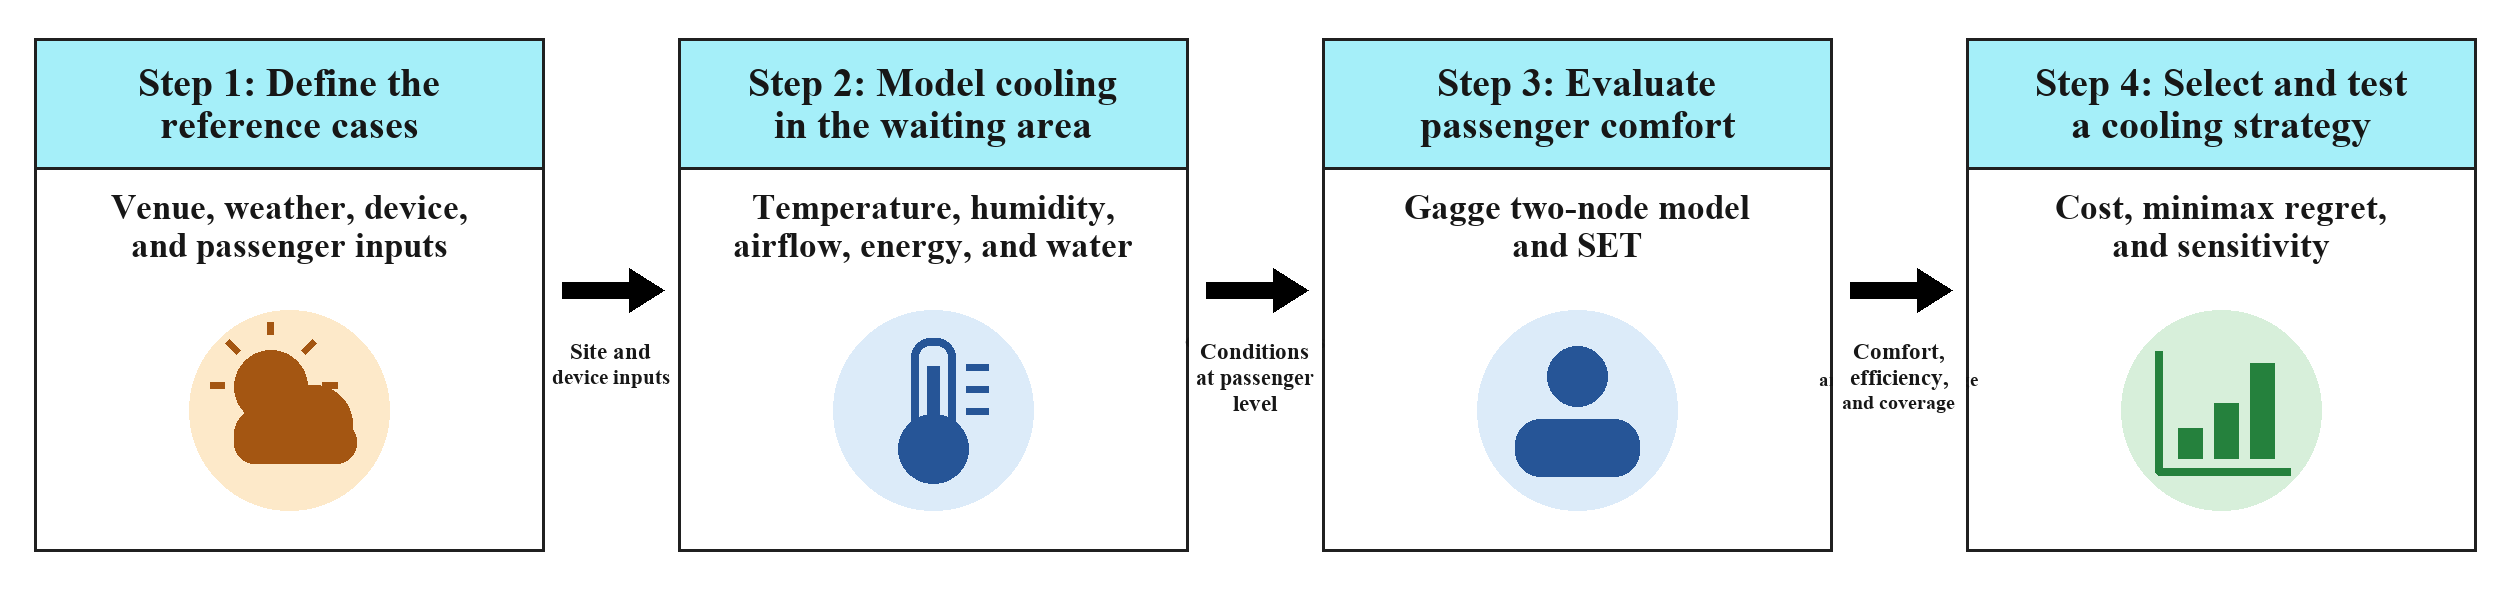
\includegraphics[width=\linewidth]{Images/action_plan_flowchart.png}
    \caption{Flowchart of the action plan.}
    \label{fig:action-plan}
\end{figure}

We used OpenAI Codex to assist with source documentation, calculation checks, and manuscript revisions~\cite{openai_codex_review}.


%% MODEL 1 %%
\section{Model I: Physical Environment and Cooling}
 
\subsection{Model Description}
 
Model I follows heat, moisture, airflow, electricity, and water. It starts with outdoor temperature, humidity, pressure, and ventilation. It then calculates the outlet air from each cooling device and mixes that air into the waiting area. The fan improves modeled comfort by increasing airspeed at the passenger~\cite{cbe_fans_2023}. The Evaporative Cooler and Large Evaporative Cooler lower the air temperature, and the zone model determines how much of that outlet cooling remains after mixing with outdoor air.
 
\subsection{Variables}
\begin{table}[H]
  \centering
  \renewcommand{\arraystretch}{1.3}
  \begin{tabularx}{\textwidth}{p{0.20\textwidth}lY}
    \toprule
    \textbf{Variable} & \textbf{Symbol} & \textbf{Description} \\
    \midrule
    Air temperature & $T, T_{out}, T_{supply}$ & Local, outdoor, and cooler supply dry-bulb temperatures ($^\circ$C). \\
    \rowcolor{gray!15} Relative humidity & $RH$ & Relative humidity of the air (\%). \\
    Vapor pressures & $p, p_v, p_{sat}$ & Total air pressure, water-vapor partial pressure, and saturation vapor pressure (Pa). \\
    \rowcolor{gray!15} Humidity ratio & $w, w_{out}, w_{supply}$ & Water vapor per unit dry air for the local, outdoor, and supply states (kg/kg). \\
    Wet-bulb temperature & $T_{wb}$ & Entering-air wet-bulb temperature ($^\circ$C). \\
    \rowcolor{gray!15} Temperature drop & $\Delta T, \Delta T_{rated}$ & Modeled and maximum stated cooler outlet temperature drops ($^\circ$C). \\
    Moist-air enthalpy & $h$ & Moist-air enthalpy per unit dry air (kJ/kg). \\
    \rowcolor{gray!15} Mass flow and specific heat & $\dot m,\dot m_{dry\ air},c_p$ & Stream mass flow and cooler dry-air mass flow (kg/s), and specific heat used in the heat balance. \\
    Evaporated water & $m_{water}$ & Water evaporated during the modeled period (kg). \\
    \rowcolor{gray!15} Ventilation inputs & $Q,C_w,A,U$ & Volumetric flow (m$^3$/s), opening effectiveness, equivalent opening area (m$^2$), and approach wind speed (m/s). \\
    Power, time, and energy & $P,\Delta t,E$ & Device electrical power (kW), modeled duration (h), and electricity consumed (kWh). \\
    \bottomrule
  \end{tabularx}
\end{table}

\subsection{Primary Equations}
 
The first step converts relative humidity into a humidity ratio $w$, which is the mass of water vapor per unit mass of dry air, using the ASHRAE relationships implemented in PsychroLib~\cite{psychrolib_volume}:
\begin{equation}
w = \frac{0.621945\, p_v}{p - p_v}, \qquad p_v = \frac{RH}{100}\, p_{sat}(T)
\end{equation}
The saturation pressure $p_{sat}$ is calculated from the ASHRAE correlation. The wet-bulb temperature $T_{wb}$ is found by solving the psychrometric energy balance. In the ideal direct-evaporation model, the entering-air wet-bulb temperature sets the lower bound for the supply temperature~\cite{pnnl_evaporative}.
 
For the selected saturation-limited model, the outlet temperature drop is
\begin{equation}
\Delta T = \min\left[\Delta T_{rated},\; T_{out} - T_{wb}\right], \qquad T_{supply} = T_{out} - \Delta T
\end{equation}
The cooler is treated as an approximately constant-enthalpy process, where the enthalpy of moist air in kJ/kg dry air is~\cite{psychrolib_volume}
\begin{equation}
h = 1.006\,T + w\,(2501 + 1.86\,T)
\end{equation}
Equating the inlet and supply enthalpies gives the supply humidity ratio directly~\cite{psychrolib_volume}:
\begin{align}
h_{out} &= 1.006T_{out}+w_{out}(2501+1.86T_{out}), \\
h_{out} &= 1.006T_{supply}+w_{supply}(2501+1.86T_{supply}), \\
w_{supply} &= \frac{h_{out}-1.006T_{supply}}{2501+1.86T_{supply}}.
\end{align}
We recover the vapor pressure and relative humidity by rearranging the humidity-ratio equation:
\begin{equation}
p_v=\frac{p\,w}{0.621945+w},
\qquad RH=100\,\frac{p_v}{p_{sat}(T)}.
\end{equation}
If the tentative outlet exceeds $100\%$ RH, we solve for the warmer outlet temperature at which the constant-enthalpy state is saturated. The added vapor carried by the supply stream is $w_{supply}-w_{out}$ per kilogram of dry air. Multiplying by dry-air flow and operating time gives the mass of water evaporated:
\begin{equation}
m_{water} = \dot{m}_{dry\ air}\,(w_{supply} - w_{out})\,(3600\,\Delta t)
\end{equation}
The waiting area uses a steady sensible-heat balance and a separate moisture balance. Let $\dot m_o$ and $\dot m_s$ denote the outdoor exchange and cooler supply flows, on a dry-air mass basis. For an evaporative cooler in the one-zone, mixing-only case, mass conservation gives an outflow of $\dot m_o+\dot m_s$. Balancing the incoming and outgoing fluxes gives
\begin{align}
(\dot m_o+\dot m_s)c_p T_{zone}
 &= \dot m_o c_p T_{out}+\dot m_s c_p T_{supply},\\
(\dot m_o+\dot m_s)w_{zone}
 &= \dot m_o w_{out}+\dot m_s w_{supply}.
\end{align}
Here $c_p=1006\,\mathrm{J/(kg\,K)}$ is the same for every stream in the model, so it cancels in the sensible-heat balance. Dividing by the total flow and subtracting from the outdoor temperature gives
\begin{equation}
 T_{out}-T_{zone}
 = \frac{\dot m_s}{\dot m_o+\dot m_s}(T_{out}-T_{supply}).
\end{equation}
This separates the cooler's own temperature drop from the fraction retained after mixing. We recover the zone RH from $T_{zone}$ and $w_{zone}$ using the same vapor-pressure relation. Electrical energy is
\begin{equation}
E = P\,\Delta t
\end{equation}
 

\subsection{Data Sources and Reference Cases}
The main weather comparison uses simultaneous NASA POWER hourly temperature, relative humidity, and pressure for June--August 2025 at the three city reference coordinates~\cite{nasa_hourly_summer_2025}. For each city, we select the hottest hour and two other hours from the hottest 10\% of records. We choose the hours with the highest and lowest humidity ratios in that subset.

The transit references are Rosa Parks Plaza and West End Station in Dallas; the Grove Hall clear-roof control shelter and Mattapan outdoor trolley waiting area in Boston; and the bus and light-rail waiting areas at Central Avenue/Camelback in Phoenix~\cite{dart_rosa,dart_west,boston_shade,bwa_mattapan,valley_bus,valley_rail}. The larger-area references are Dallas College Mountain View Student Courtyard and the Love Field curbside canopy, Boston University's George Sherman Union Courtyard and Logan Terminal C canopy, and ASU's Delph Courtyard and Sky Harbor Terminal 3 canopy~\cite{dallas_college_student_courtyard,dal_lovefield_canopy,bu_gsu_courtyard,bos_logan_canopy,asu_delph_courtyard,phx_skyharbor_canopy}.

Ventilation and baseline passenger airspeed are scenario estimates. The wind-driven relation $Q=C_w A U$ and the urban wind-profile exponent are drawn from EnergyPlus; equivalent apertures and passenger sheltering factors are analyst assumptions~\cite{energyplus_wind_ventilation,energyplus_242_surface}. The estimates use the city summer-mean wind references, and the enlarged courtyard/canopy openings are documented project choices~\cite{nasa_2026_dallas_summer,nasa_2026_boston_summer,nasa_2026_phoenix_summer}.

Contest systems A, B and C use powers of 0.25, 1.2 and 2.5 kW, with stated maxima of 3$^\circ$C perceived cooling, 5$^\circ$C air cooling and 8$^\circ$C air cooling, respectively~\cite{comap_2026_problem_b}. Reference products are the 20-inch AirEye fan and Portacool APEX 2000/4000 coolers. The recorded reference prices are \$1,499, \$4,159 and \$4,939; the selected cooler flows are 9,000 and 13,350 CFM~\cite{aireye_20_price,portacool_2000,portacool_4000}. The fan exposure uses a selected 357 ft/min contour value from the AirEye sheet~\cite{aireye_2021_specs}.

\subsection{Key Assumptions and Justifications}
 
\begin{table}[H]
  \centering
  \renewcommand{\arraystretch}{1.3}
  \begin{tabularx}{\textwidth}{lYp{0.66\textwidth}}
    \toprule
    \textbf{\#} & \textbf{Assumption} & \multicolumn{1}{c}{\textbf{Justification}} \\
    \midrule
    \nextassumption\label{assumption:model1-1} & The waiting area is one well-mixed zone. & The model uses one air temperature and humidity value for the occupied zone. \\
    \rowcolor{gray!15} \nextassumption\label{assumption:model1-2} & The default model accounts for heat and moisture carried by air exchange. & This isolates the effect of air exchange using the available inputs. \\
    \nextassumption\label{assumption:model1-3} & Evaporative cooling follows a constant-enthalpy process. & This is a standard ideal model for direct evaporation. Field performance depends on the unit and its operating conditions. \\
    \rowcolor{gray!15} \nextassumption\label{assumption:model1-4} & Cooling is limited by the wet-bulb temperature and saturation. & This prevents impossible outlet states. It is justified by thermodynamics and is more credible than applying the rated temperature drop in all weather. \\
    \nextassumption\label{assumption:model1-5} & Rated power and airflow represent the candidate devices. & Common reference specifications let us compare options consistently. Field results depend on equipment condition and placement. \\
    \rowcolor{gray!15} \nextassumption\label{assumption:model1-6} & Each modeled period lasts one hour. & This creates comparable energy and water totals. \\
    \bottomrule
  \end{tabularx}
\end{table}
 

\subsection{Conclusion}
 
Model I is a useful first-principles screening model. It is strongest when comparing broad resource and weather effects, such as why evaporative cooling works better in dry air and why a fan uses less energy. It is weaker at predicting the exact temperature at a particular bench. The dry-air balance closed in all 144 runs. We set passenger airspeed to $1.81\,\mathrm{m/s}$ for the fan and use venue baseline airspeed for the other options. Field measurements could test the airspeed at different passenger positions and capture airflow from the coolers.
 

%% MODEL 2 %% 

\section{Model II: Human Thermal Comfort Using the Gagge Model}
\subsection{Model Description}
 
How hot a person feels depends on air temperature, airflow, humidity, and radiant heat. Air movement can increase heat loss from the skin at a fixed air temperature. Humidity can reduce sweat evaporation. Radiant heat from a roof or pavement can make a person warmer than the air suggests. Model II combines these effects into the Standard Effective Temperature, or SET~\cite{ashrae_thermal_comfort_2025}.
 
We represent the body with two thermal compartments, an internal core and a skin layer. Heat moves from the core to the skin and from the skin through clothing to the surroundings. The model accounts for sweating, changes in skin blood flow, convection, radiation, respiration, and evaporation~\cite{ashrae_thermal_comfort_2025,comf_0112_set}.
 
\subsection{Variables}
\begin{table}[H]
  \centering
  \renewcommand{\arraystretch}{1.3}
  \begin{tabularx}{\textwidth}{p{0.20\textwidth}lY}
    \toprule
    \textbf{Variable} & \textbf{Symbol} & \textbf{Description} \\
    \midrule
    Standard Effective Temperature & $SET, SET_{upper}$ & Equivalent comfort temperature and its upper comparison target ($^\circ$C). \\
    \rowcolor{gray!15} Thermoregulatory coefficients & $c_{sw}, c_{dil}, c_{str}$ & Coefficients for sweating, vasodilation, and vasoconstriction in the two-node model. \\
    Exposure duration & $\Delta t$ & Duration of the modeled comfort exposure (h). \\
    \rowcolor{gray!15} Hot-discomfort loss & $L, L_{none}, L_{option}$ & Degree-hours above the upper target for a given case, the baseline, or the active option. \\
    Hot-discomfort reduction & $B$ & Decrease in hot-discomfort loss relative to the no-device baseline ($^\circ$C$\cdot$h). \\
    \rowcolor{gray!15} Electricity & $E, E_i$ & Electricity used by the device, with $i$ indexing the option (kWh). \\
    Discomfort reduction per kWh & $\eta$ & Hot-discomfort reduction divided by electricity used ($^\circ$C$\cdot$h/kWh). \\
    \bottomrule
  \end{tabularx}
\end{table}

\subsection{Primary Equations and Calculation Idea}
 
The complete Gagge model is an iterative physiological heat-balance model. Its central idea can be written as two energy balances~\cite{cbe_two_node}:
\begin{align}
\text{Core storage} &= \text{metabolic heat} - \text{external work} - \text{respiration} - \text{heat sent from core to skin} \\
\text{Skin storage} &= \text{heat received from core} - \text{convection} - \text{radiation} - \text{evaporation}
\end{align}
To see how the weather enters those two balances, write the storage rates per unit body area as
\begin{align}
K_{cr}\frac{dT_{cr}}{dt}
 &= M-W-q_{res}-q_{cr\to sk},\\
K_{sk}\frac{dT_{sk}}{dt}
 &= q_{cr\to sk}-q_{dry}-q_{evap}.
\end{align}
Here $K_{cr}$ and $K_{sk}$ are heat capacities per unit body area, $M$ is metabolic heat production, $W$ is external work, and $q_{res}$ combines sensible and latent respiratory losses. Adding the balances cancels the internal core-to-skin transfer. It leaves the sum of the two storage rates equal to $M-W-q_{res}-q_{dry}-q_{evap}$~\cite{ashrae_thermal_comfort_2025}.

For sensible exchange, convection and radiation act in parallel at the outer clothing surface. Clothing adds a series resistance $R_{cl}$. Eliminating the clothing surface temperature gives
\begin{equation}
 T_{op}=\frac{h_c T_a+h_r T_r}{h_c+h_r},
 \qquad
 q_{dry}=\frac{T_{sk}-T_{op}}{R_{cl}+1/[f_{cl}(h_c+h_r)]},
\end{equation}
where $T_a$ and $T_r$ are air and mean radiant temperatures, $h_c$ and $h_r$ are the convective and radiative coefficients, and $f_{cl}$ is the ratio of clothed to bare body area. With skin wettedness $w_{sk}$ and combined evaporative resistance $R_e$, the evaporative exchange is
\begin{equation}
 q_{evap}=w_{sk}\,\frac{p_{sat}(T_{sk})-p_a}{R_e}.
\end{equation}
Here $p_a$ is ambient vapor pressure. Higher airspeed changes the convective coefficient and the resistance to evaporation. Higher ambient vapor pressure reduces the driving difference for evaporation~\cite{ashrae_thermal_comfort_2025}. This is how a fan or an evaporative cooler can shift the modeled comfort response through different inputs.

Core and skin temperatures affect the body's control responses. If the body becomes warm, the model increases skin blood flow and sweating. If it becomes cold, it reduces skin blood flow and can add shivering heat. We use the documented control coefficients~\cite{comf_0112_set}:
\begin{equation}
c_{sw} = 170, \qquad c_{dil} = 120, \qquad c_{str} = 0.5
\end{equation}
After simulating the body, SET is defined as the temperature of a standard reference environment that would cause the same skin temperature and skin wettedness as the actual environment~\cite{ashrae_thermal_comfort_2025}. The actual inputs are air temperature, mean radiant temperature, airspeed, humidity, pressure, clothing, activity, posture, body size, and exposure time.
 
At the end of the exposure, the SET calculation uses the simulated skin temperature and wettedness. In the standard environment the air and radiant temperatures are both $SET$ and relative humidity is $50\%$. Equating the skin heat loss in that environment to the modeled value gives the scalar equation~\cite{ashrae_thermal_comfort_2025,comf_0112_set}:
\begin{equation}
 q_{dry}+q_{evap}=
 \frac{T_{sk}-SET}{R_{d,std}}
 +w_{sk}\,\frac{p_{sat}(T_{sk})-0.5\,p_{sat}(SET)}{R_{e,std}},
\end{equation}
where $R_{d,std}$ and $R_{e,std}$ are the standard environment's total sensible and evaporative resistances. We solve for SET for each device and for the no-device baseline. For the one-hour comparison, the excess above the upper target is constant over the scoring period, giving the hot-discomfort loss:
\begin{equation}
L = \Delta t \cdot \max\left(0,\; SET - SET_{upper}\right)
\end{equation}
For the current comparison, $SET_{upper} = 26^\circ$C. The benefit is the reduction in loss relative to no device, and dividing that benefit by energy gives the reduction in hot discomfort per kWh:
\begin{equation}
B = L_{none} - L_{option}, \qquad \eta = \frac{B}{E}
\end{equation}
 
Section~\ref{sec:efficiency} uses raw SET reduction, $(SET_{\rm none}-SET_i)/E_i$, to compare the full temperature-equivalent change per kWh at the reference position. The two efficiency measures agree numerically for a one-hour case when both SET values are above the upper target. The hot-discomfort measure stops crediting additional cooling once SET reaches the upper target.

\subsection{Key Assumptions and Justifications}
 
\begin{table}[H]
  \centering
  \renewcommand{\arraystretch}{1.3}
  \begin{tabularx}{\textwidth}{lYp{0.66\textwidth}}
    \toprule
    \textbf{\#} & \textbf{Assumption} & \multicolumn{1}{c}{\textbf{Justification}} \\
    \midrule
    \nextassumption\label{assumption:model2-1} & One reference person represents the comparison. & The person is seated, 171 cm, 70 kg, at 1 met, with no external work. This gives a consistent basis when actual passenger demographics are unavailable. \\
    \rowcolor{gray!15} \nextassumption\label{assumption:model2-2} & Clothing is 0.36 clo. & This represents shorts and a short-sleeved shirt and is suitable for a hot-weather comparison. Actual riders will wear different clothing~\cite{ashrae_2021_comfort}. \\
    \nextassumption\label{assumption:model2-3} & Exposure lasts 60 minutes. & The Gagge model is time-dependent, so an exposure period is required. Sixty minutes gives us a common exposure period for comparisons. \\
    \rowcolor{gray!15} \nextassumption\label{assumption:model2-4} & Radiant temperature uses an air-reference approximation. & It is held at the uncooled outdoor reference temperature across options. Holding radiant temperature fixed isolates the effect of the device on air conditions. \\
    \nextassumption\label{assumption:model2-5} & The $23$--$26^\circ$C SET band is a policy band. & It provides a common comparison rule. Compliance and population satisfaction require separate assessments. \\
    \rowcolor{gray!15} \nextassumption\label{assumption:model2-6} & The model represents an average healthy adult response. & This provides a common basis for comparing modeled comfort. Assessing heat risk for vulnerable passengers requires separate evidence~\cite{cbe_two_node}. \\
    \bottomrule
  \end{tabularx}
\end{table}

\subsection{Conclusion}

Model II gives the Fan and both evaporative coolers a common measure of thermal comfort for the reference occupant. Differences in airflow, humidity, and radiant conditions can change SET even at the same air temperature. A safety assessment would also need to account for the exposure and characteristics of the people using the venue.


\section{Optimizing Cooling of Various Stations}
\label{sec:efficiency}

The fan delivered the most cooling per kilowatt-hour in all 36 modeled venue and weather combinations. It also led per dollar of equipment purchase price in 25 cases. The larger evaporative cooler led in the other 11.

We measured cooling as the reduction in Standard Effective Temperature (SET) from the no-device case at the same venue and under the same weather. We divided this reduction by electricity used during the modeled hour and by equipment purchase price. The 36 cases cover four venue types in Dallas, Boston, and Phoenix, each under peak-temperature, hot-humid, and hot-dry conditions.

\begin{figure}[H]
    \centering
    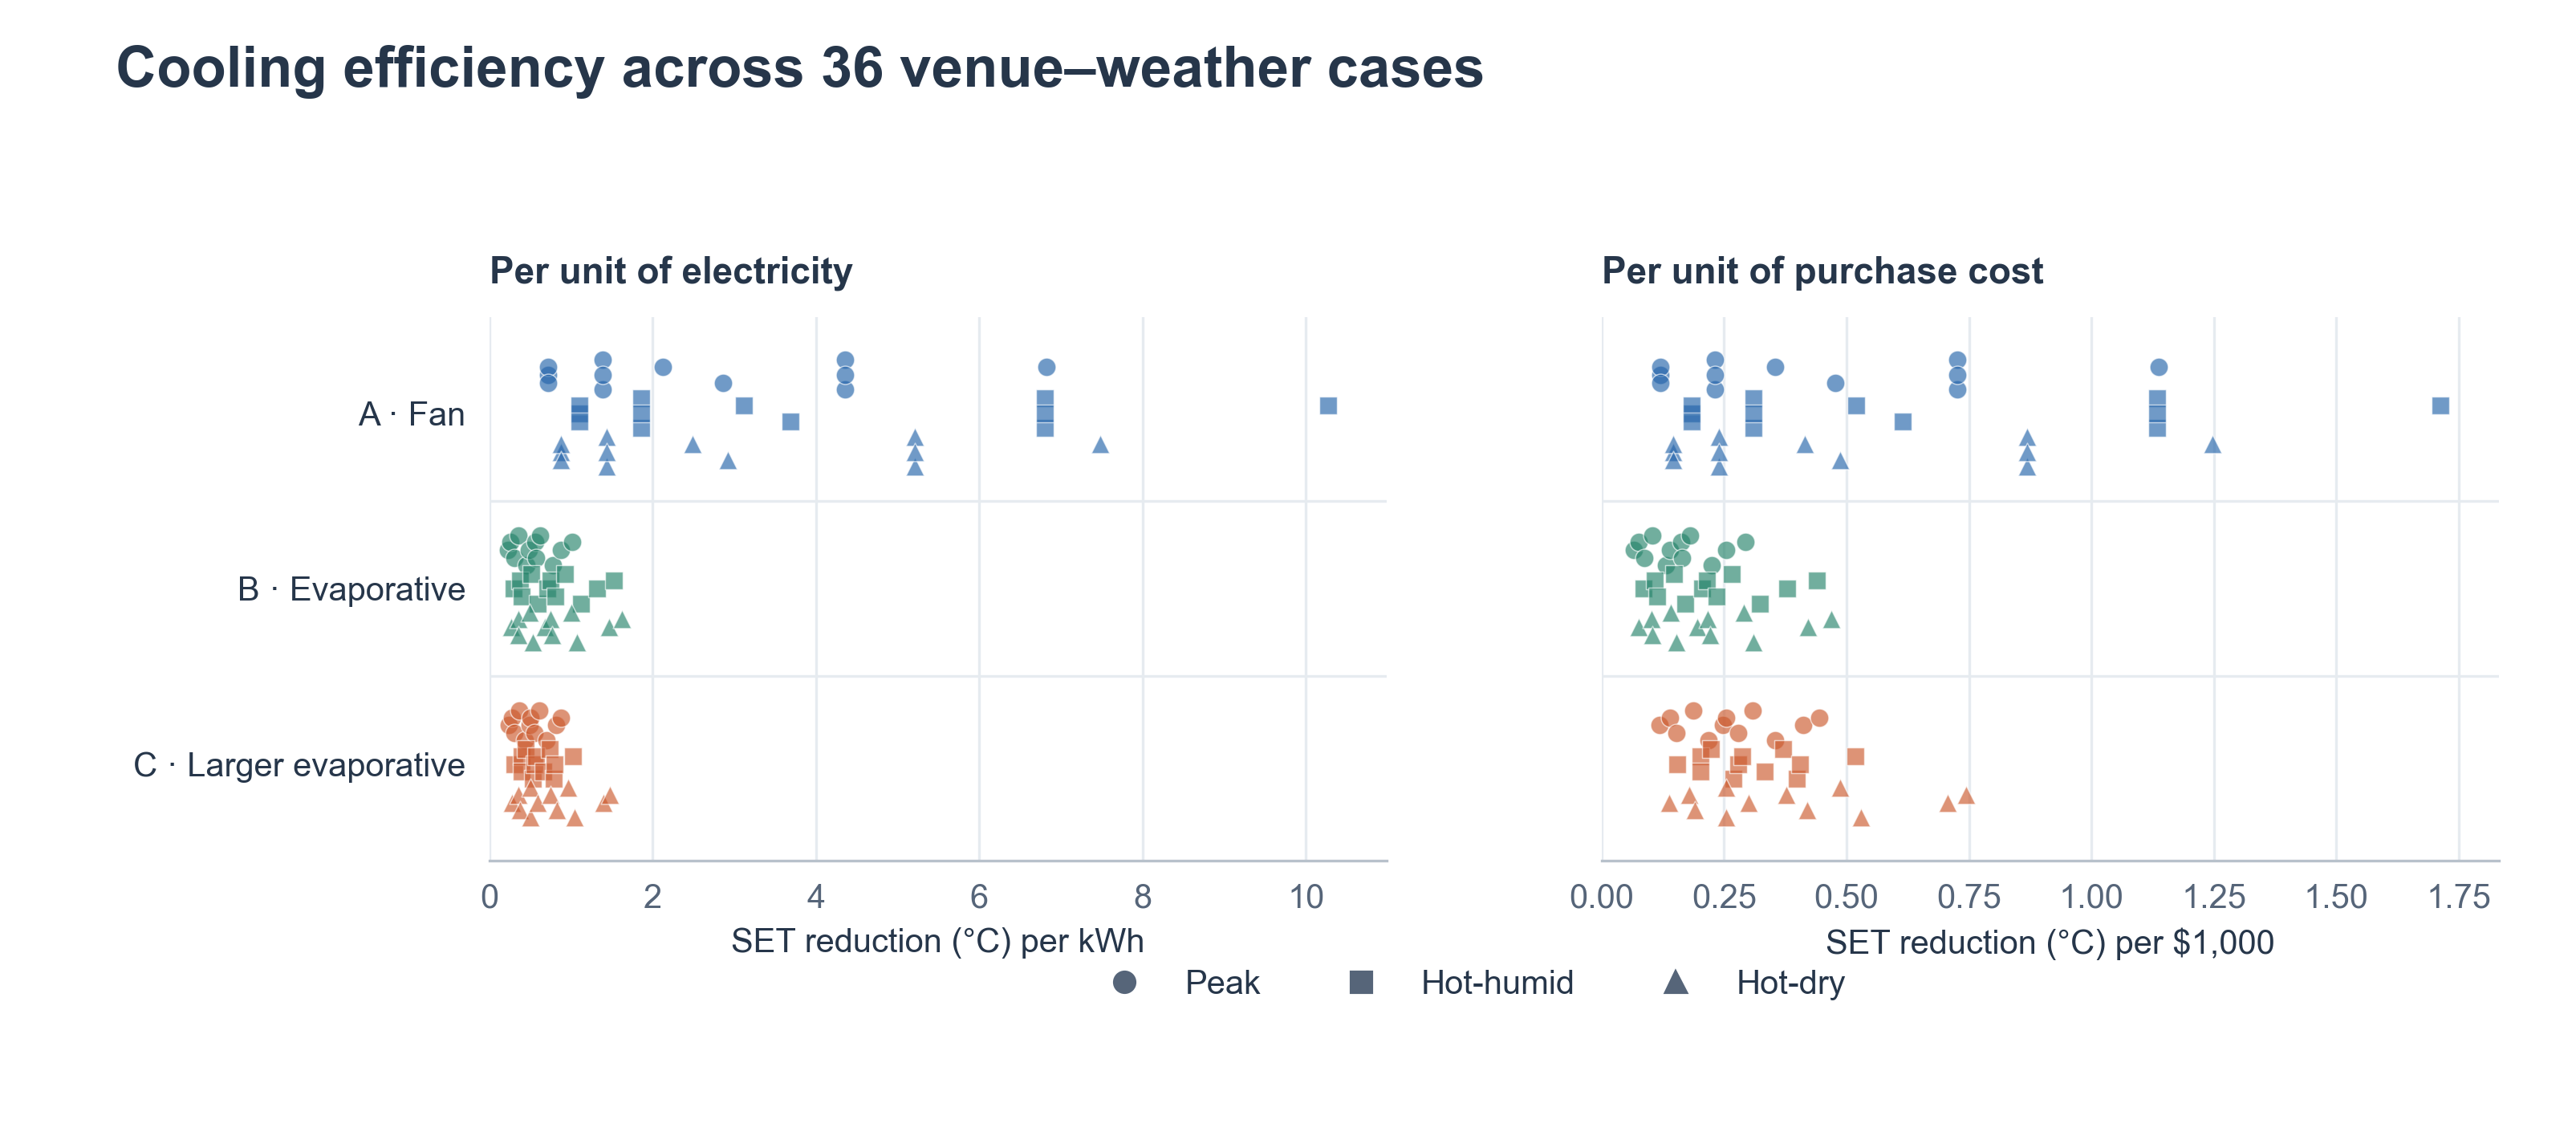
\includegraphics[width=0.94\linewidth]{Images/F6_efficiency_all_cases.png}
    \caption{Cooling per kWh and per \$1,000 of equipment purchase price across all 36 cases.}
    \label{fig:efficiency}
\end{figure}

The fan delivered 1.14 to 9.59 times the cooling per kWh of the more efficient evaporative cooler in the same case. The advantage was smallest at the Dallas rail platform in the hot-dry scenario and largest under the Boston airport canopy in the hot-humid scenario.

\subsection{Adapting the Bus-Shelter Model to Rail}
For Dallas, the modeled rail platform uses 5.81 kg/s of dry-air exchange and a baseline passenger airspeed of 1.40 m/s, compared with 2.18 kg/s and 0.93 m/s at the bus shelter. These are scenario estimates based on different equivalent openings and sheltering factors. We hold weather, equipment, and exposure duration fixed within the city so the comparison reflects the two airflow assumptions.

The higher outdoor exchange dilutes the evaporative cooler's supply air. The higher rail baseline airspeed also leaves less scope for a fan modeled at the same operating airspeed at both sites. The peak-hour figures below show both effects. Using separate airflow assumptions lets the model compare the two layouts. Field measurements would be needed to test its accuracy at either location.

\subsection{Purchase Price and Peak Hour Cooling}

Option C led per purchase dollar in ten Dallas cases and at the Phoenix rail platform in hot-dry weather. At the Dallas rail platform it led in all three scenarios. The fan led throughout Boston. These comparisons use upfront equipment price.

During peak heat, the Dallas bus shelter fan reduced SET by 0.53\ensuremath{^{\circ}\mathrm{C}} using 0.25 kWh, compared with 1.75\ensuremath{^{\circ}\mathrm{C}} using 2.50 kWh for the larger cooler. At the Dallas rail platform, the same devices reduced SET by 0.18\ensuremath{^{\circ}\mathrm{C}} and 1.38\ensuremath{^{\circ}\mathrm{C}}, respectively. At both sites the extra 2.25 kWh delivered about 1.2\ensuremath{^{\circ}\mathrm{C}} more cooling.

\begin{figure}[H]
    \centering
    \begin{subfigure}[t]{0.43\textwidth}
        \centering
        \vspace{0pt}
        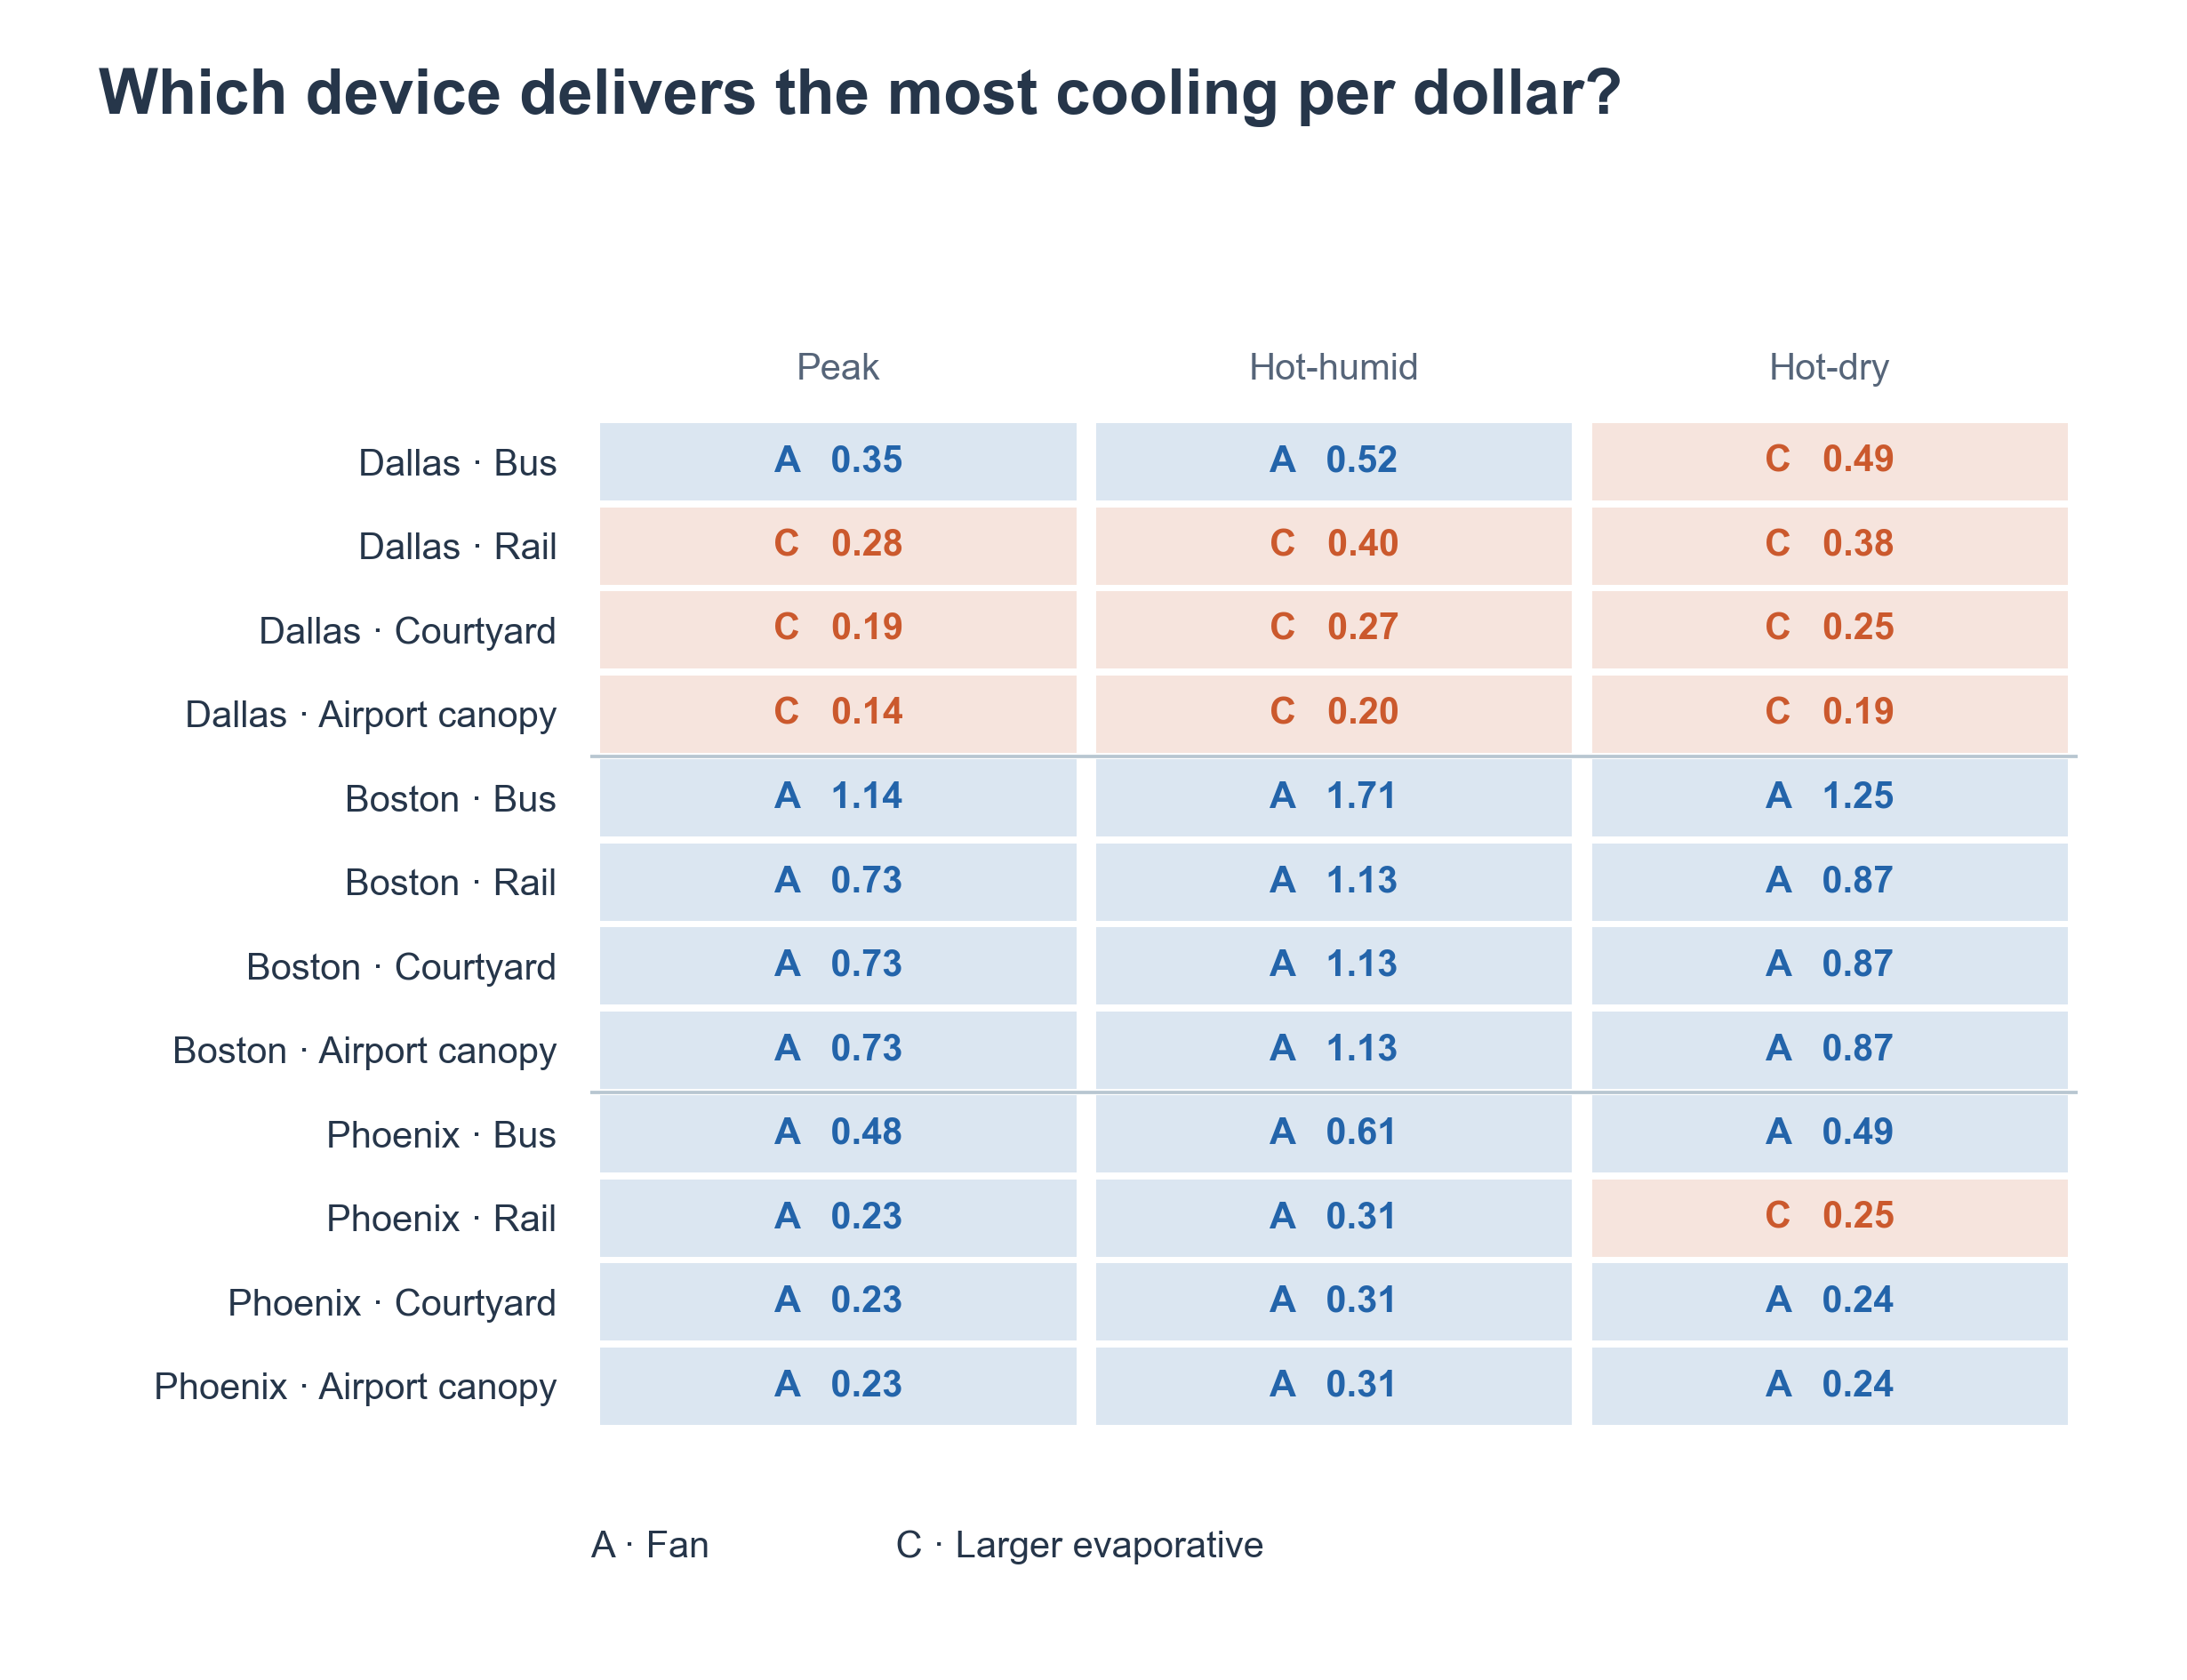
\includegraphics[width=\linewidth]{Images/F9_purchase_efficiency_winners.png}
        \caption{Purchase-price efficiency leader by venue and weather. The number is SET reduction in degrees Celsius per \$1,000.}
        \label{fig:purchase-efficiency}
    \end{subfigure}
    \hfill
    \begin{subfigure}[t]{0.54\textwidth}
        \centering
        \vspace{0pt}
        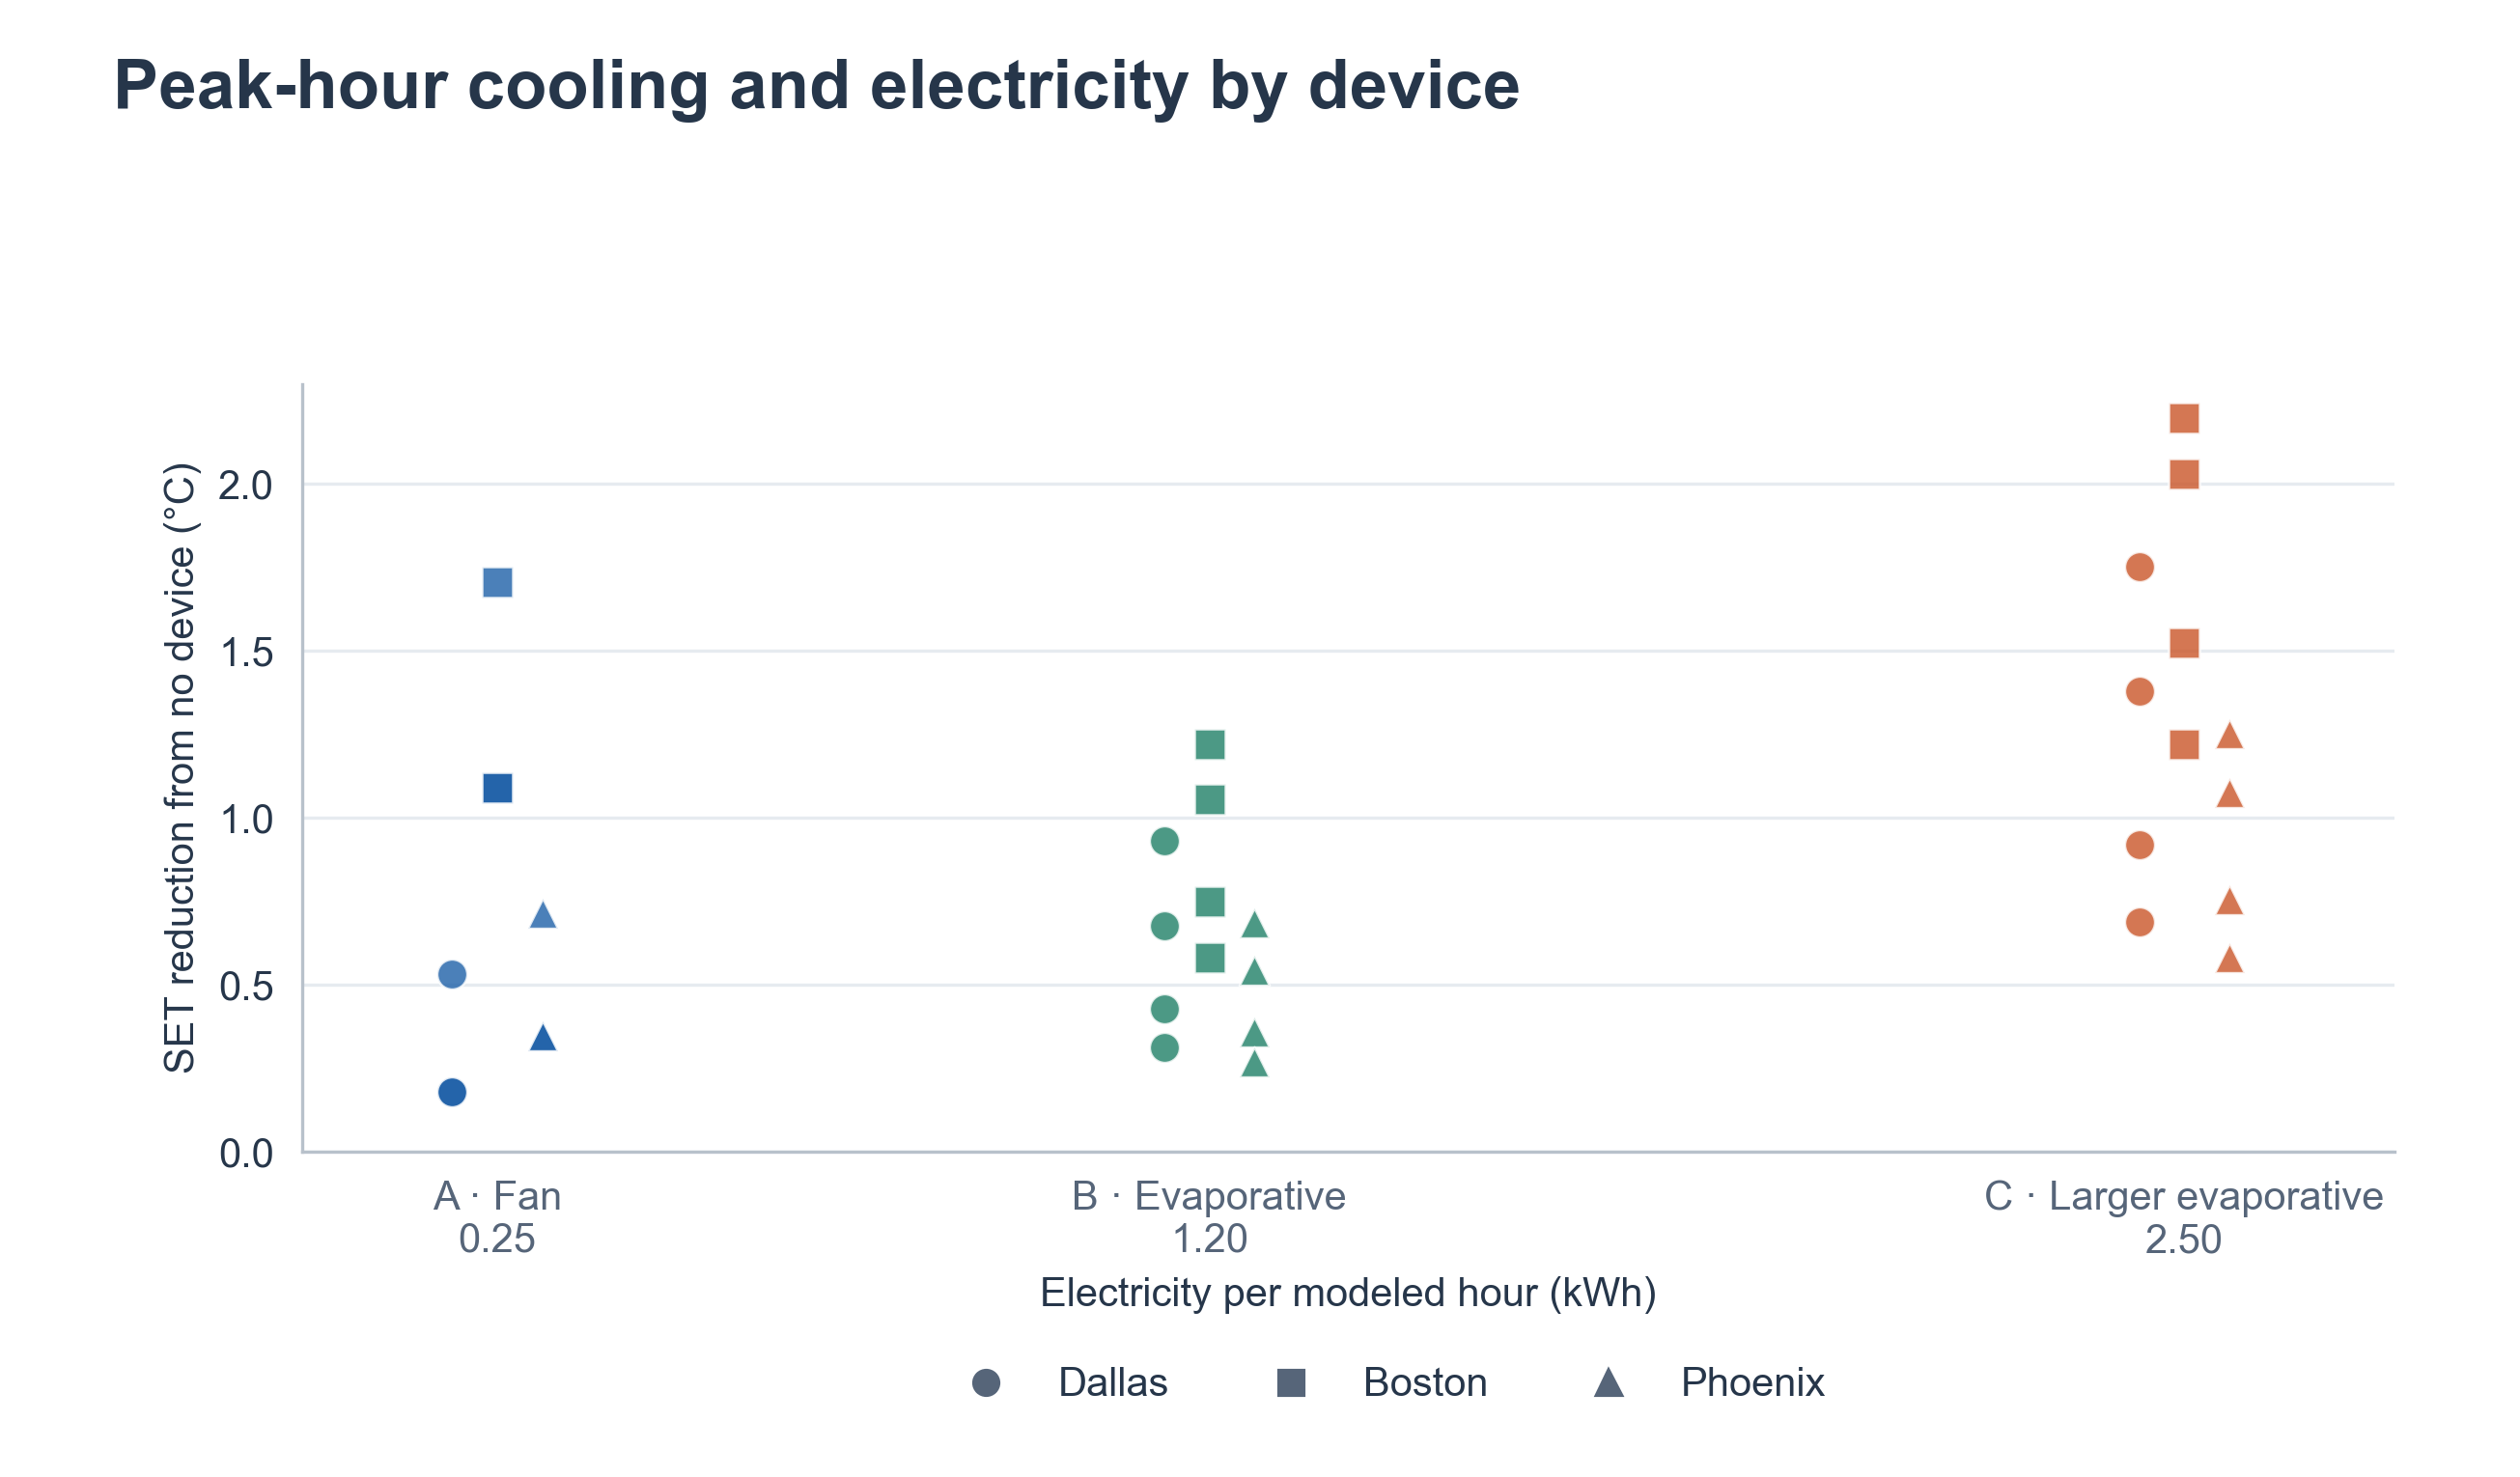
\includegraphics[width=\linewidth]{Images/F10_peak_cooling_electricity.png}
        \caption{Peak-hour SET reduction and electricity use. Each device has the same electricity use at all venues in the one-hour comparison.}
        \label{fig:peak-electricity}
    \end{subfigure}
    \caption{Purchase-price efficiency and peak-hour electricity tradeoffs.}
    \label{fig:purchase-and-peak}
\end{figure}

\subsection{Fan Efficiency and Outdoor Air Exchange}

\begin{figure}[H]
    \centering
    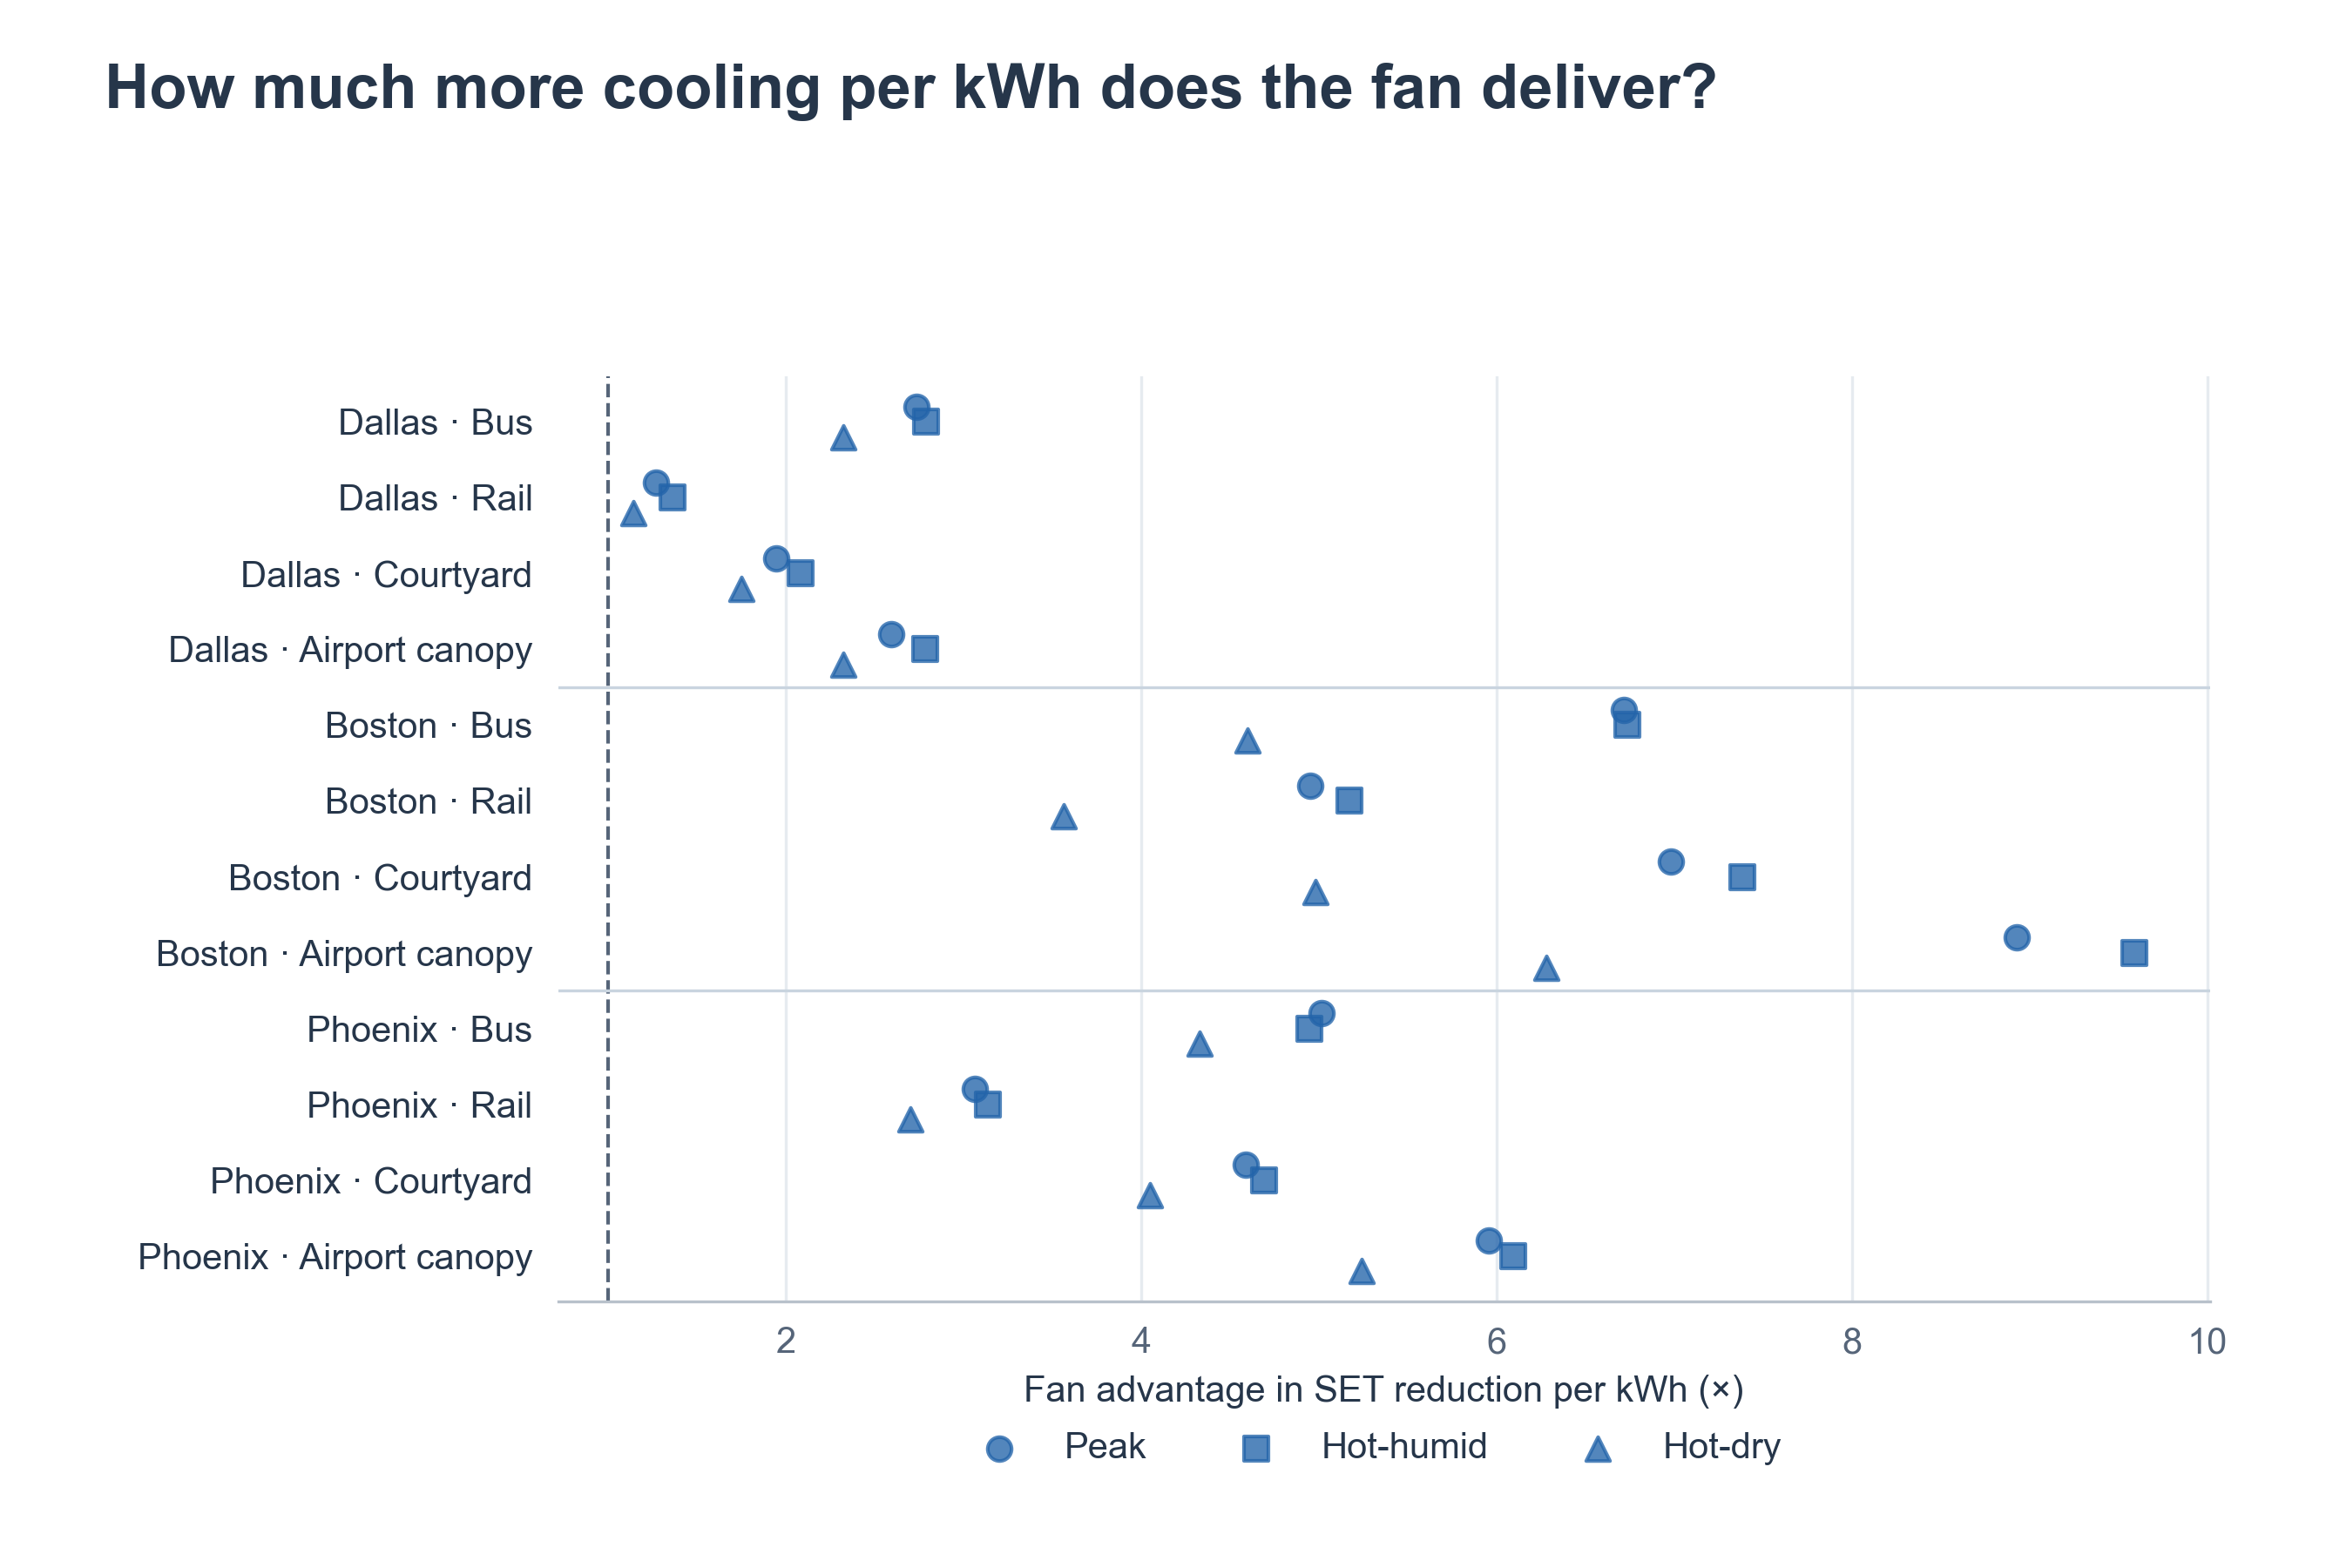
\includegraphics[width=0.66\linewidth]{Images/F12_fan_efficiency_advantage.png}
    \caption{Fan energy efficiency divided by the better evaporative cooler in each case.}
    \label{fig:fan-advantage}
\end{figure}

We used a separate summer-mean reference case to test how outdoor air exchange affects efficiency at the six courtyards and airport canopies. We multiplied the reference exchange rate by two and four while holding the number of devices, their power, and the fan airspeed at the reference person fixed.

\begin{figure}[H]
    \centering
    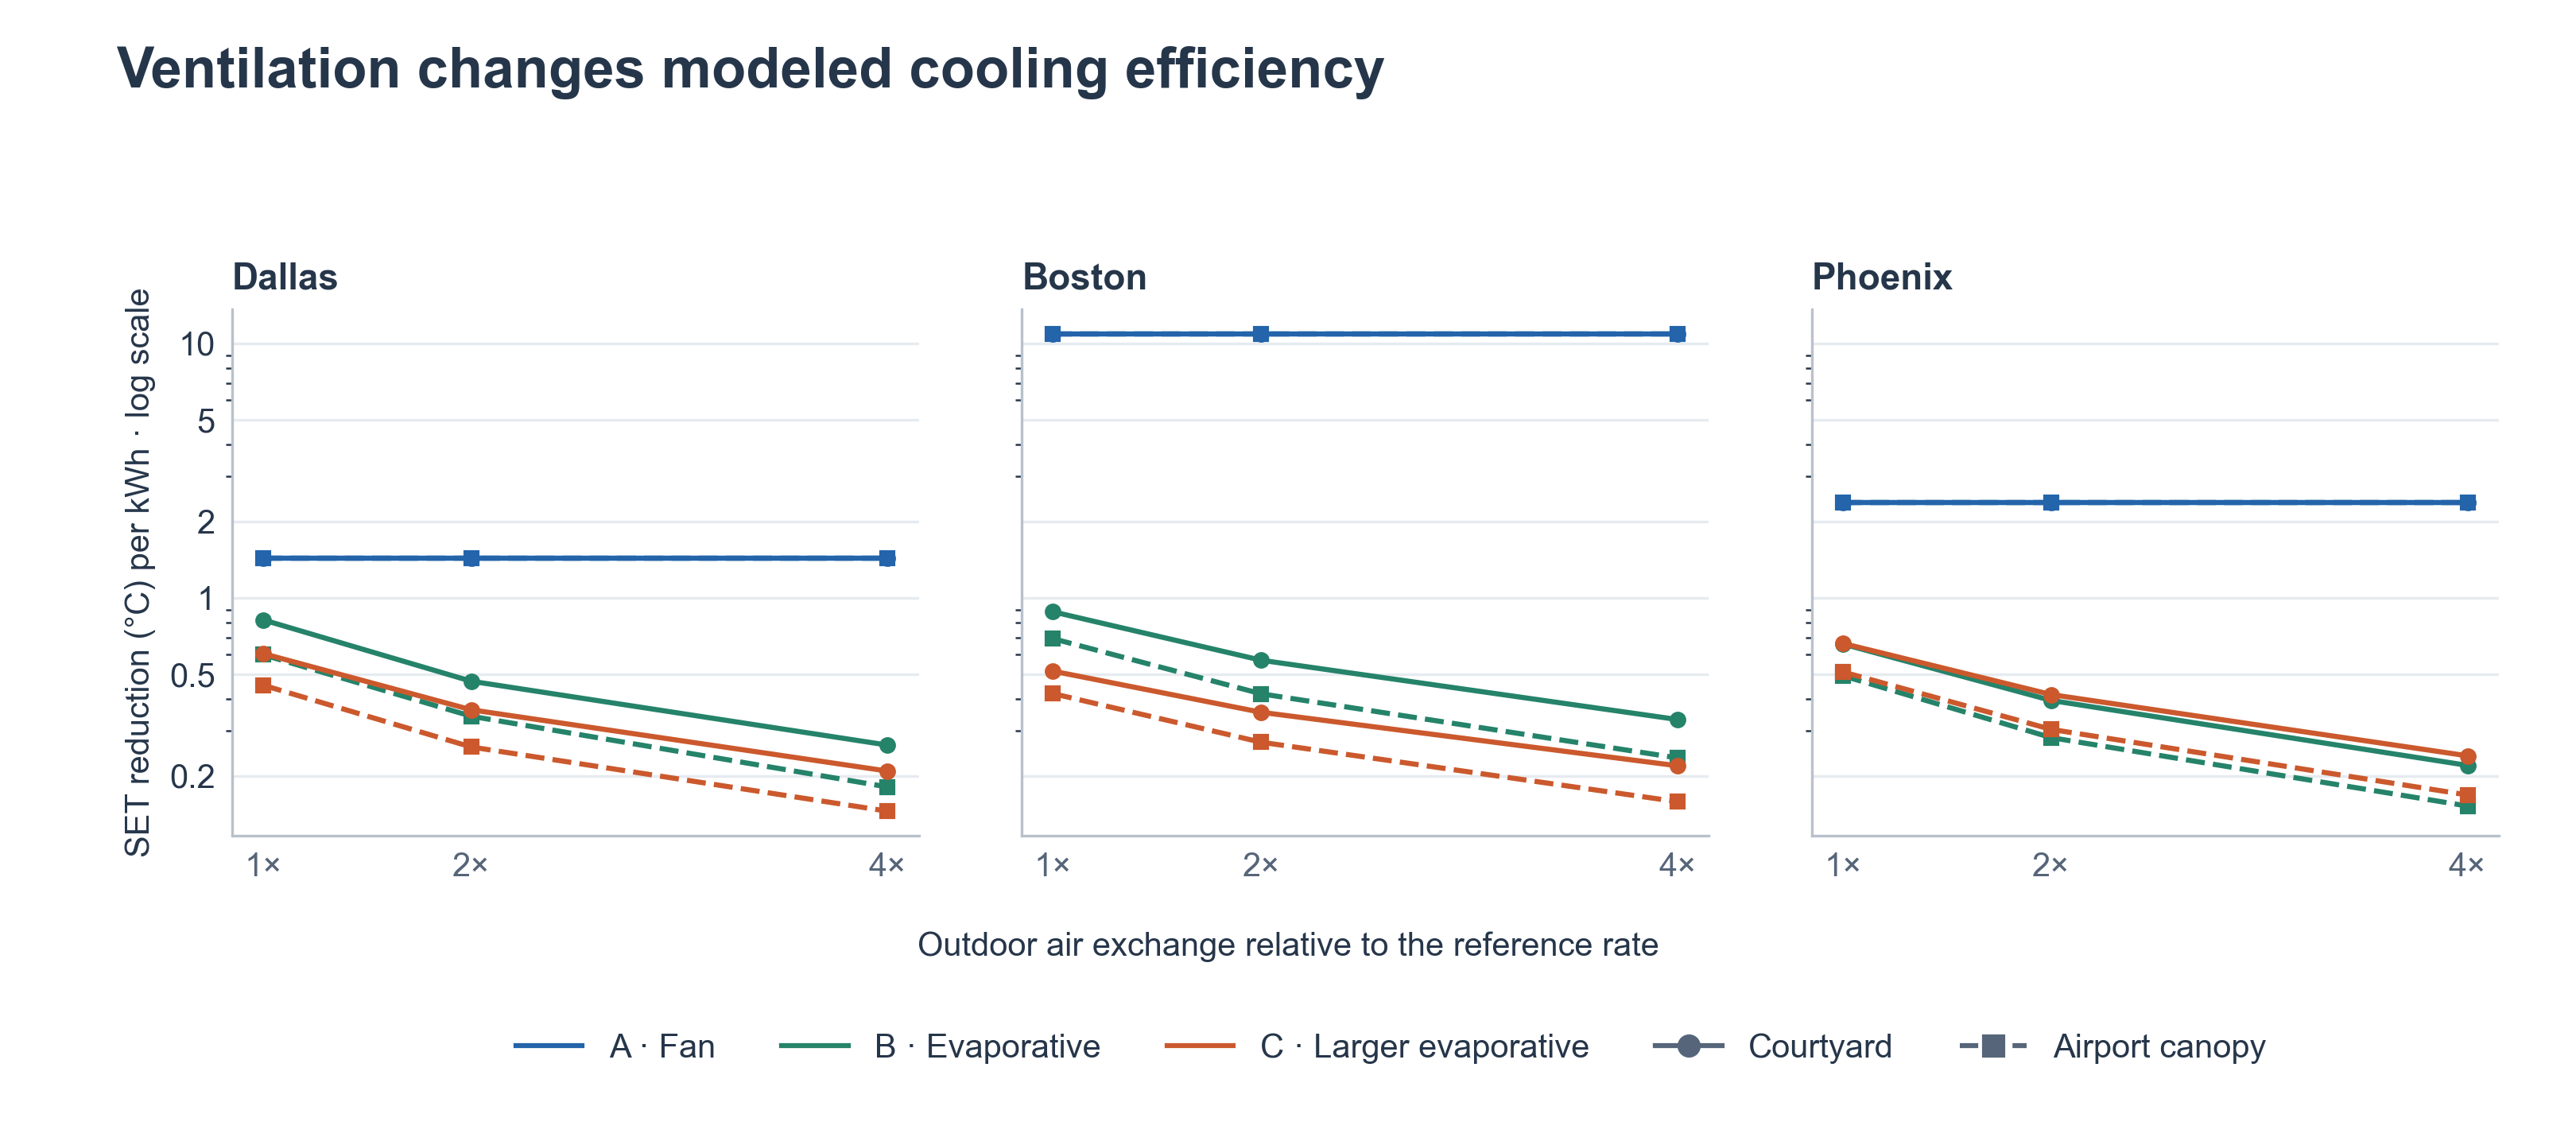
\includegraphics[width=0.9\linewidth]{Images/F11_ventilation_efficiency.png}
    \caption{Cooling efficiency as outdoor air exchange increases. The vertical axis is logarithmic.}
    \label{fig:ventilation-efficiency}
\end{figure}

Evaporative cooling efficiency declined as more outdoor air mixed into the occupied zone. At the Dallas courtyard, quadrupling exchange reduced the larger cooler's SET benefit from 1.51\ensuremath{^{\circ}\mathrm{C}} to 0.52\ensuremath{^{\circ}\mathrm{C}}, a decrease of about 65\%. Its electricity use remained at 2.50 kWh, so its efficiency fell from 0.60 to 0.21\ensuremath{^{\circ}\mathrm{C}} per kWh.

The fan curves are flat because the sweep holds passenger-position airspeed fixed. The courtyard and canopy fan curves overlap within each city because they use the same reference airspeed. The sweep isolates the model's response to exchange and describes a single reference position at each venue.

%% MODEL 3 %% 

\section{Model III: Cost, Feasibility, and Minimax Regret}
\subsection{Model Description}
 
Model III turns the physical and comfort results into a decision. It checks whether each option has a valid model solution and whether it meets any active cost, electricity, or water limits. It then compares the options in three hot-weather scenarios. It selects the option with the smallest worst-case regret across the three scenarios.
 
\subsection{Variables}
\begin{table}[H]
  \centering
  \renewcommand{\arraystretch}{1.3}
  \begin{tabularx}{\textwidth}{p{0.20\textwidth}lY}
    \toprule
    \textbf{Variable} & \textbf{Symbol} & \textbf{Description} \\
    \midrule
    Equipment option & $i,j$ & Candidate option and index used to compare feasible alternatives. \\
    \rowcolor{gray!15} Weather scenario & $s$ & Peak-temperature, hot-humid, or hot-dry scenario. \\
    Hot-discomfort loss & $L_{i,s}$ & Modeled discomfort for option $i$ in scenario $s$ ($^\circ$C$\cdot$h). \\
    \rowcolor{gray!15} Scenario regret & $R_{i,s}$ & Excess loss over the best feasible option in that scenario ($^\circ$C$\cdot$h). \\
    Maximum regret & $R_{i,\max}$ & Largest scenario regret for an option ($^\circ$C$\cdot$h). \\
    \rowcolor{gray!15} Recommended option & $i^*$ & Feasible option that minimizes maximum regret. \\
    Equipment capital cost & $C$ & Upfront equipment cost in dollars. \\
    \bottomrule
  \end{tabularx}
\end{table}

\subsection{Primary Equations}
 
We use the minimax-regret decision criterion, applied here to discomfort loss~\cite{savage1951}. First define the set of physically valid options in weather scenario $s$ as $V_s$. Let $C_{i,s}$, $E_{i,s}$, and $m_{water,i,s}$ be the active cost, electricity use, and water use. Given limits on these resources, the scenario's feasible set is
\begin{equation}
 F_s=\left\{i\in V_s:
   C_{i,s}\le C_{cap},\quad
   E_{i,s}\le E_{cap},\quad
   m_{water,i,s}\le m_{cap}\right\}.
\end{equation}
We compare each resource use with the corresponding limit. The set of devices that can be recommended across all modeled weather is $F=\bigcap_s F_s$. Each scenario still has its own benchmark, $L_s^*=\min_{j\in F_s}L_{j,s}$. After observing the weather an operator could choose any device in $F_s$, so $L_s^*$ is the best attainable loss in that scenario. Subtracting that benchmark from the loss for a fixed option $i$ gives the regret
\begin{equation}
R_{i,s} = L_{i,s} - \min_{j\ \text{feasible}} L_{j,s}
\end{equation}
An option has zero regret if it is best in that scenario. Its worst regret is
\begin{equation}
R_{i,\max} = \max_{s} R_{i,s}
\end{equation}
The minimax recommendation is the robust option with the smallest upper bound on its scenario regrets. For a fixed option, the smallest valid bound $z$ is its largest scenario regret:
\begin{equation}
 \min_z\{z: z\ge L_{i,s}-L_s^* \text{ for every }s\}
 = \max_s(L_{i,s}-L_s^*)=R_{i,\max}.
\end{equation}
Minimizing that bound over the robust set gives
\begin{equation}
i^{*} \in \arg\min_{i\in F}\; R_{i,\max}
\end{equation}
We use equipment purchase prices as the cost measure for the comparative analysis.
 
\subsection{Choice of Decision Criterion}
 
TOPSIS ranks choices by their distance from an ideal point and a worst point. Its usual weighted formulation normalizes the criteria and assigns criterion weights~\cite{hwang_yoon1981}. We considered four criteria: cost, energy, water, and comfort. Those choices can strongly affect the result, especially when the units are different. A TOPSIS score can look precise even when the weights are subjective.
 
We use minimax regret to compare each choice with the best choice available under each weather scenario. The model screens options against resource limits and ranks the feasible options by discomfort regret. Each limit can stay in its original units.
 
At Grove Hall, the Large Evaporative Cooler leads on comfort and requires \$4,939 upfront, 2.50 kWh per hour, and up to about 84.1 kg of water in a modeled hour. Under illustrative limits of \$4,500, 1.50 kWh per hour, and 40 kg of water per hour, maximum regret among feasible choices is zero for the Fan, 0.49 SET degree-hours for the Small Evaporative Cooler, and 1.71 for no cooling.
 
\subsection[Key Assumptions]{Key Assumptions and Justifications}
 
\begin{table}[H]
  \centering
  \renewcommand{\arraystretch}{1.3}
  \begin{tabularx}{\textwidth}{lYp{0.66\textwidth}}
    \toprule
    \textbf{\#} & \textbf{Assumption} & \multicolumn{1}{c}{\textbf{Justification}} \\
    \midrule
    \nextassumption\label{assumption:model3-1} & The three selected weather scenarios represent the uncertainty of interest. & Peak, humid-hot, and dry-hot hours provide contrasting stresses. Each case tests an operating condition. \\
    \rowcolor{gray!15} \nextassumption\label{assumption:model3-2} & Regret is based on hot-discomfort loss. & We compare discomfort after screening options for resource feasibility. \\
    \nextassumption\label{assumption:model3-3} & An option must be feasible in every scenario to be robust. & This avoids recommending a device that fails under one supplied condition. \\
    \rowcolor{gray!15} \nextassumption\label{assumption:model3-4} & Purchase cost is the selected cost basis. & It is available and easy to compare. It omits maintenance and long-term utility costs. \\
    \nextassumption\label{assumption:model3-5} & Resource limits describe the venue. & Purchase cost, electricity, and water can each have a separate limit. \\
    \rowcolor{gray!15} \nextassumption\label{assumption:model3-6} & Scenarios enter the decision unweighted. & The largest regret across the three hours determines the ranking. \\
    \bottomrule
  \end{tabularx}
\end{table}

\subsection{Conclusion}

Minimax regret identifies the equipment choice whose largest shortfall from the scenario benchmark is smallest. We use the comfort ranking as a benchmark. The Grove Hall example shows how local limits on purchase cost, electricity, and water alter the options available to minimax.

The scenario benchmark matters because the hour with the highest discomfort can differ from the hour with the largest regret. Discomfort measures how far SET remains above the comfort target. Regret measures how much of that discomfort another feasible device could have avoided. A severe hour can leave substantial discomfort under every device and still produce a small gap between them. An hour with a lower baseline can determine the equipment choice if one option delivers substantially more relief than the others. Tracking both quantities shows where equipment choice has the greatest effect and where the venue faces a larger cooling problem.

We also distinguish a purchase decision from an operating decision. A purchase commits the venue to equipment that must be useful across the selected weather cases. During operation, staff can respond to the conditions that occur in a given hour. They can leave equipment off when the baseline meets the target and use the resource estimates to weigh additional cooling when discomfort remains. The next section reports the purchase comparison across all twelve venues.


\section{Expanding the Model for Effectiveness}

The Large Evaporative Cooler was the unique minimax choice at all 12 venues in the comfort benchmark. It had the lowest modeled hot-discomfort loss outright in 28 of 36 cases and tied for the lowest in the other eight.

Hot-discomfort loss counts SET degree-hours above $26\,^\circ\mathrm{C}$. In Boston's hot-dry case, the Large Evaporative Cooler produces $20.77\,^\circ\mathrm{C}$ SET and receives zero loss. The separate operating rule leaves cooling off when the baseline is already in the $23$--$26\,^\circ\mathrm{C}$ comfort band.

We compare each option's hot-discomfort loss with the lowest feasible loss in the same hour. We then select the option with the smallest maximum regret across the three weather cases, including no cooling in the comparison.

The baseline also puts the regret of the Fan in context. At Grove Hall, the largest shortfall with no cooling is 2.20 SET degree-hours, compared with 0.49 with the Fan. At Rosa Parks Plaza, the corresponding values are 2.56 and 1.78. The declines in maximum regret are about 1.71 and 0.78 SET degree-hours, respectively. Each of these comparisons uses the worst case for each option, which can occur in a different hour. Therefore, the difference between the two maxima describes how much installing the Fan reduces the worst shortfall across the three cases. A location with the larger baseline shortfall can gain less from the same upgrade. The site-level comparison helps identify where using only a fan would still leave a substantial gap between the available cooling and the best modeled outcome.

At Boston and Phoenix bus shelters, the Fan stays much closer to the best case than it does in Dallas. Its maximum regret is $0.49$ SET degree-hours at Grove Hall and $0.75$ at Central Avenue/Camelback, compared with $1.78$ at Rosa Parks Plaza. The hour that determines this gap also varies by site. Boston's gap occurs at peak temperature, while the hot-dry hour determines the maximum for the Dallas and Phoenix bus fans.

\begin{figure}[H]
    \centering
    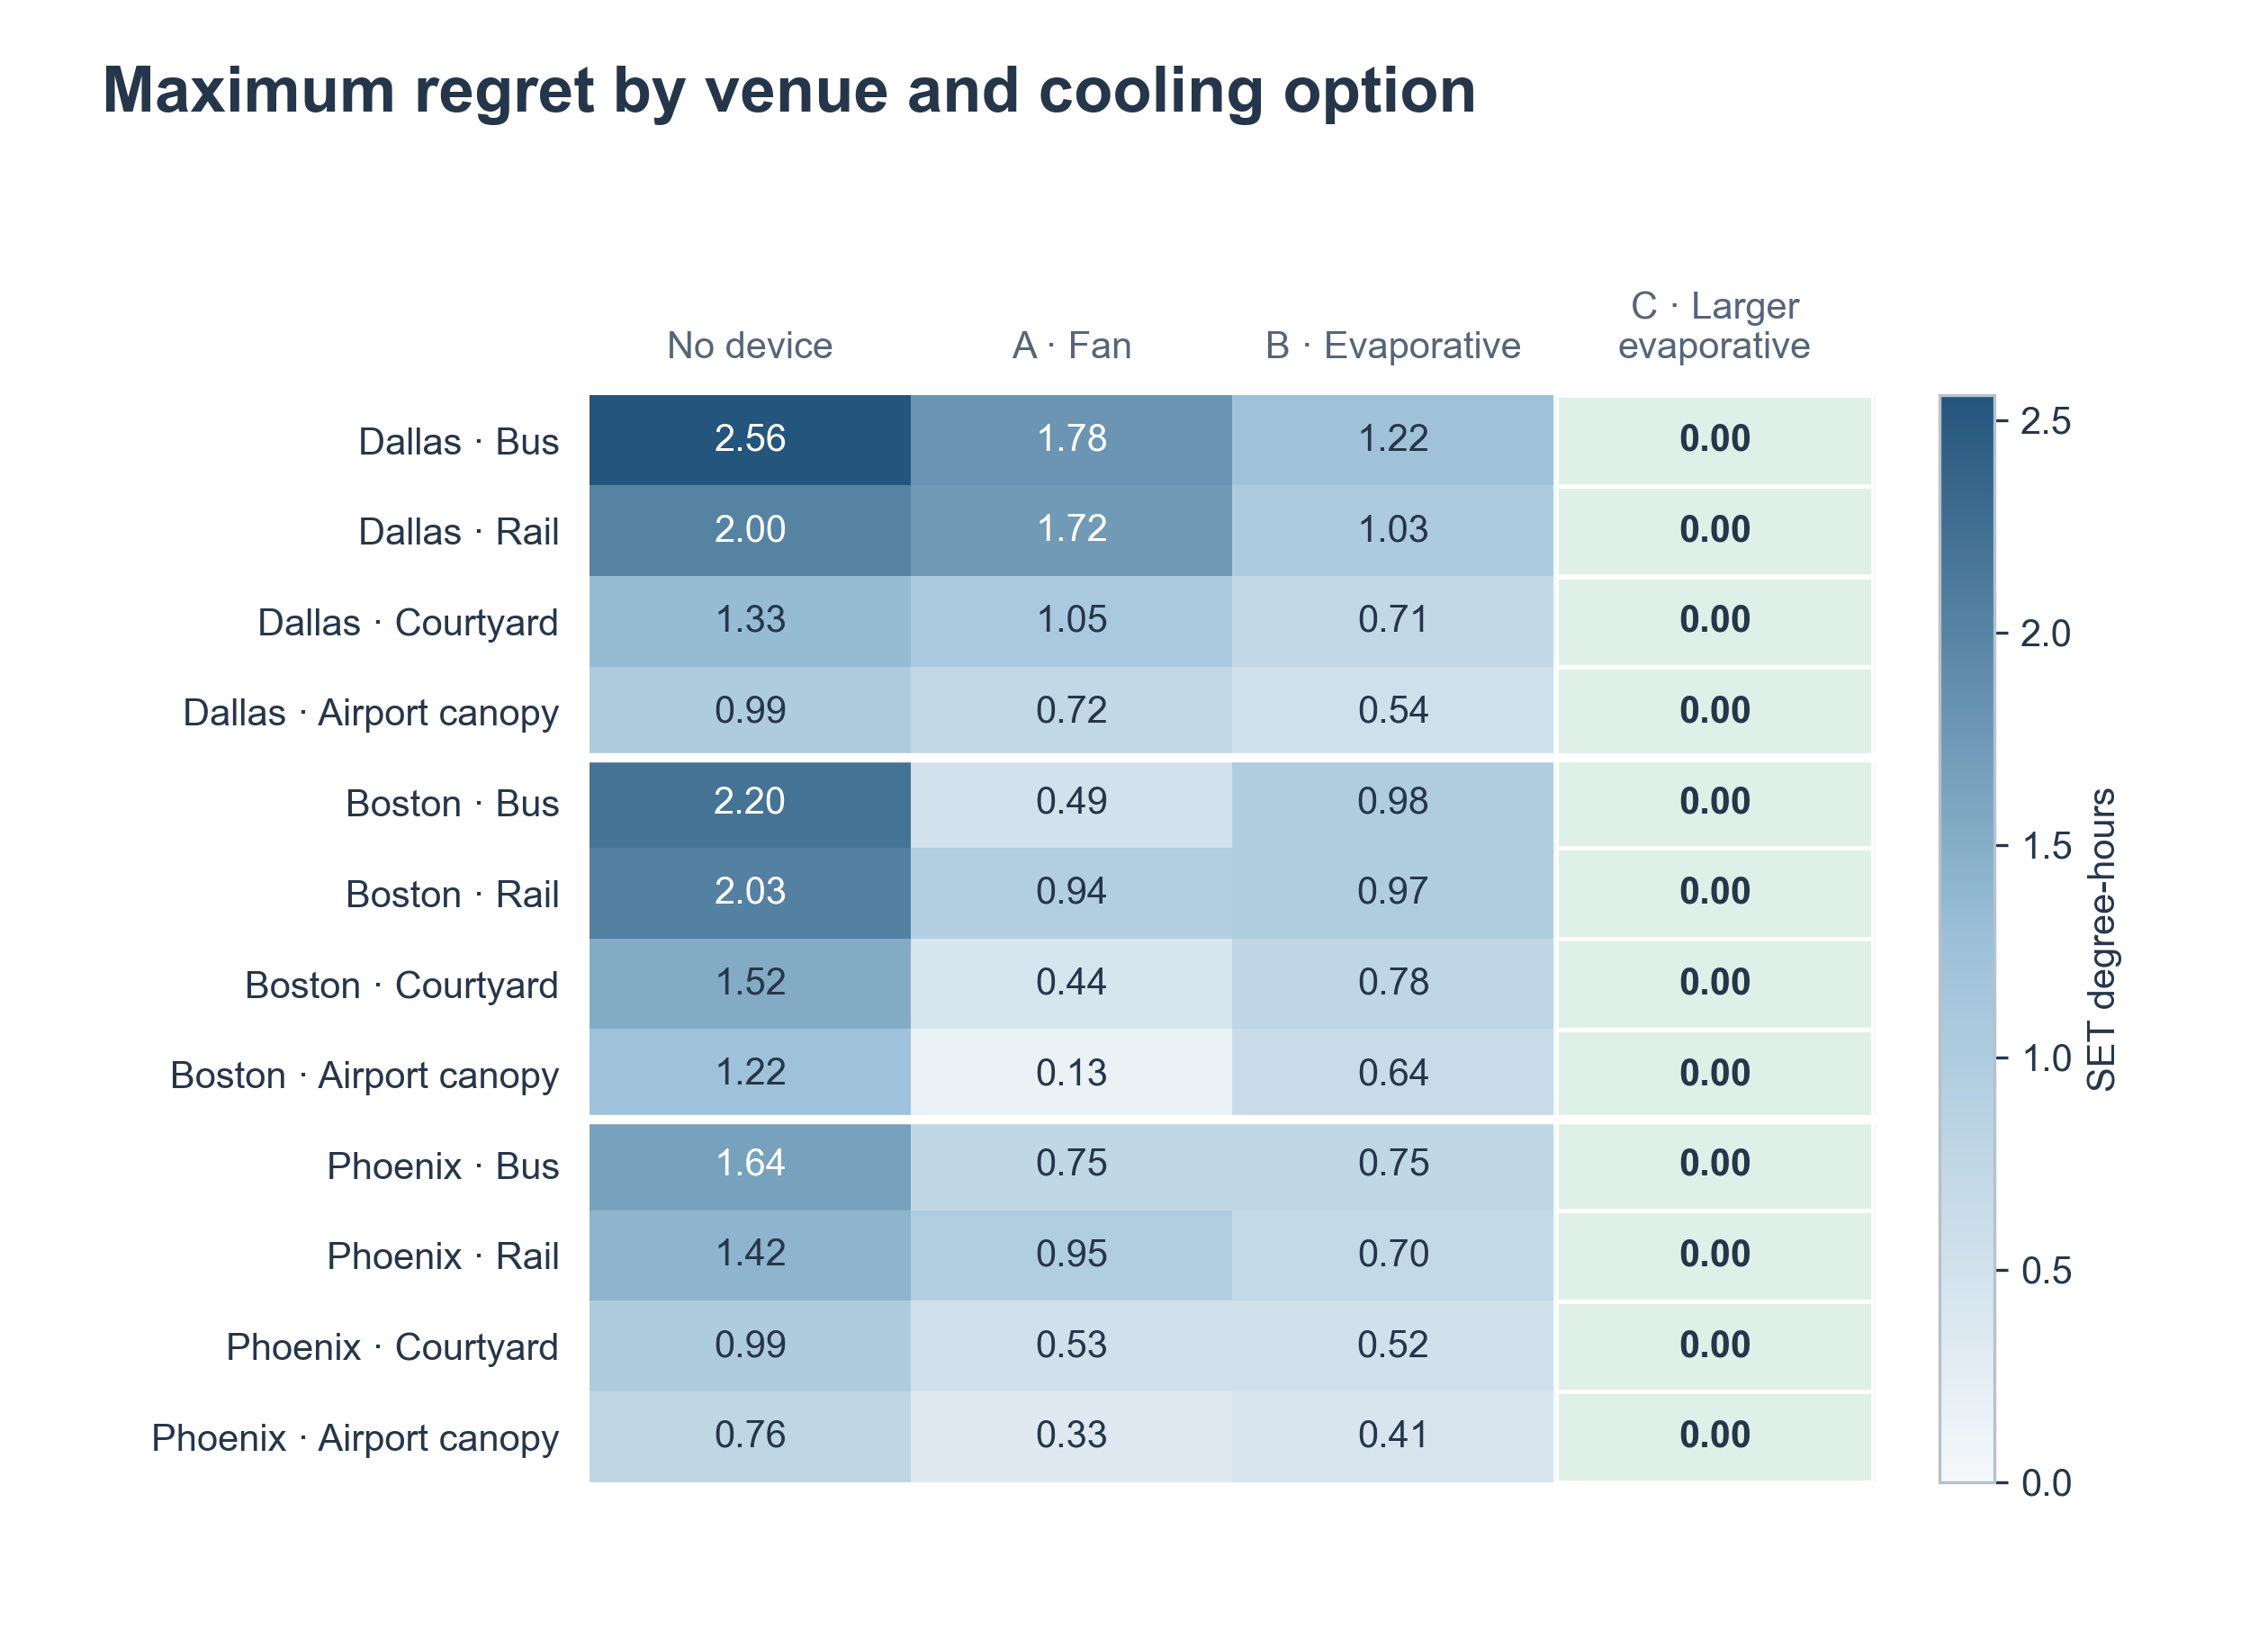
\includegraphics[width=0.88\linewidth,trim=0 0 0 69.12bp,clip]{Images/F7_maximum_regret_all_venues.png}
    \caption{Maximum regret in SET degree-hours across the three modeled scenarios. Green cells identify the comfort benchmark winner.}
    \label{fig:max-regret}
\end{figure}

At the Dallas bus shelter, maximum regret was 1.78 SET degree-hours for the Fan and 1.22 for the Small Evaporative Cooler. At the Dallas rail platform, the corresponding values were 1.72 and 1.03. The Large Evaporative Cooler had zero maximum regret at both sites.

In the comfort benchmark at Grove Hall, the Fan's maximum regret is about half that of the Small Evaporative Cooler ($0.49$ versus $0.98$ SET degree-hours). At the Phoenix bus shelter, both options round to $0.75$, so the Fan gives nearly identical worst-case regret with lower electricity use and zero evaporation. At the Phoenix rail platform, the Small Evaporative Cooler reduces the maximum regret from $0.95$ to $0.70$. Venue-level airflow therefore matters even when nearby sites share the same weather inputs.

Absolute comfort tells a second part of the story. At the Phoenix bus shelter, the Large Evaporative Cooler leaves peak-hour SET at $33.68\,^\circ\mathrm{C}$, almost $8\,^\circ\mathrm{C}$ above the comparison target. Its zero regret reflects its lead among the tested options. The remaining heat discomfort is still substantial.

\subsection{Resource Tradeoffs at Bus Shelters}

The Dallas bus and rail radars share the same axis scales. Both sites use the same equipment and share city weather, so their modeled resource inputs coincide. The different regret profiles reflect how those devices perform under each venue's airflow assumptions. For Dallas at peak temperature, the added relief from switching from the Fan to the Large Evaporative Cooler is about $1.22\,^{\circ}\mathrm{C}$ of SET at the bus shelter and $1.20\,^{\circ}\mathrm{C}$ at the rail platform. The extra electricity is $2.25$ kWh at either site. Across the three scenarios, the Small Evaporative Cooler's maximum regret is $1.22$ at the bus shelter and $1.03$ at the platform. The similar peak-hour upgrades and different maximum regrets show why we compare the full set of weather cases. The shared radar scales make the size of the regret differences directly comparable between venues. On the resource spokes, the paths align because we use the same device specifications and outdoor weather within Dallas. Each spoke represents a separate outcome. We read the regret spoke first to identify the minimax choice, then read the other spokes to see what it takes to achieve that result in purchase cost, electricity, and evaporated water.

\begin{figure}[H]
    \centering
    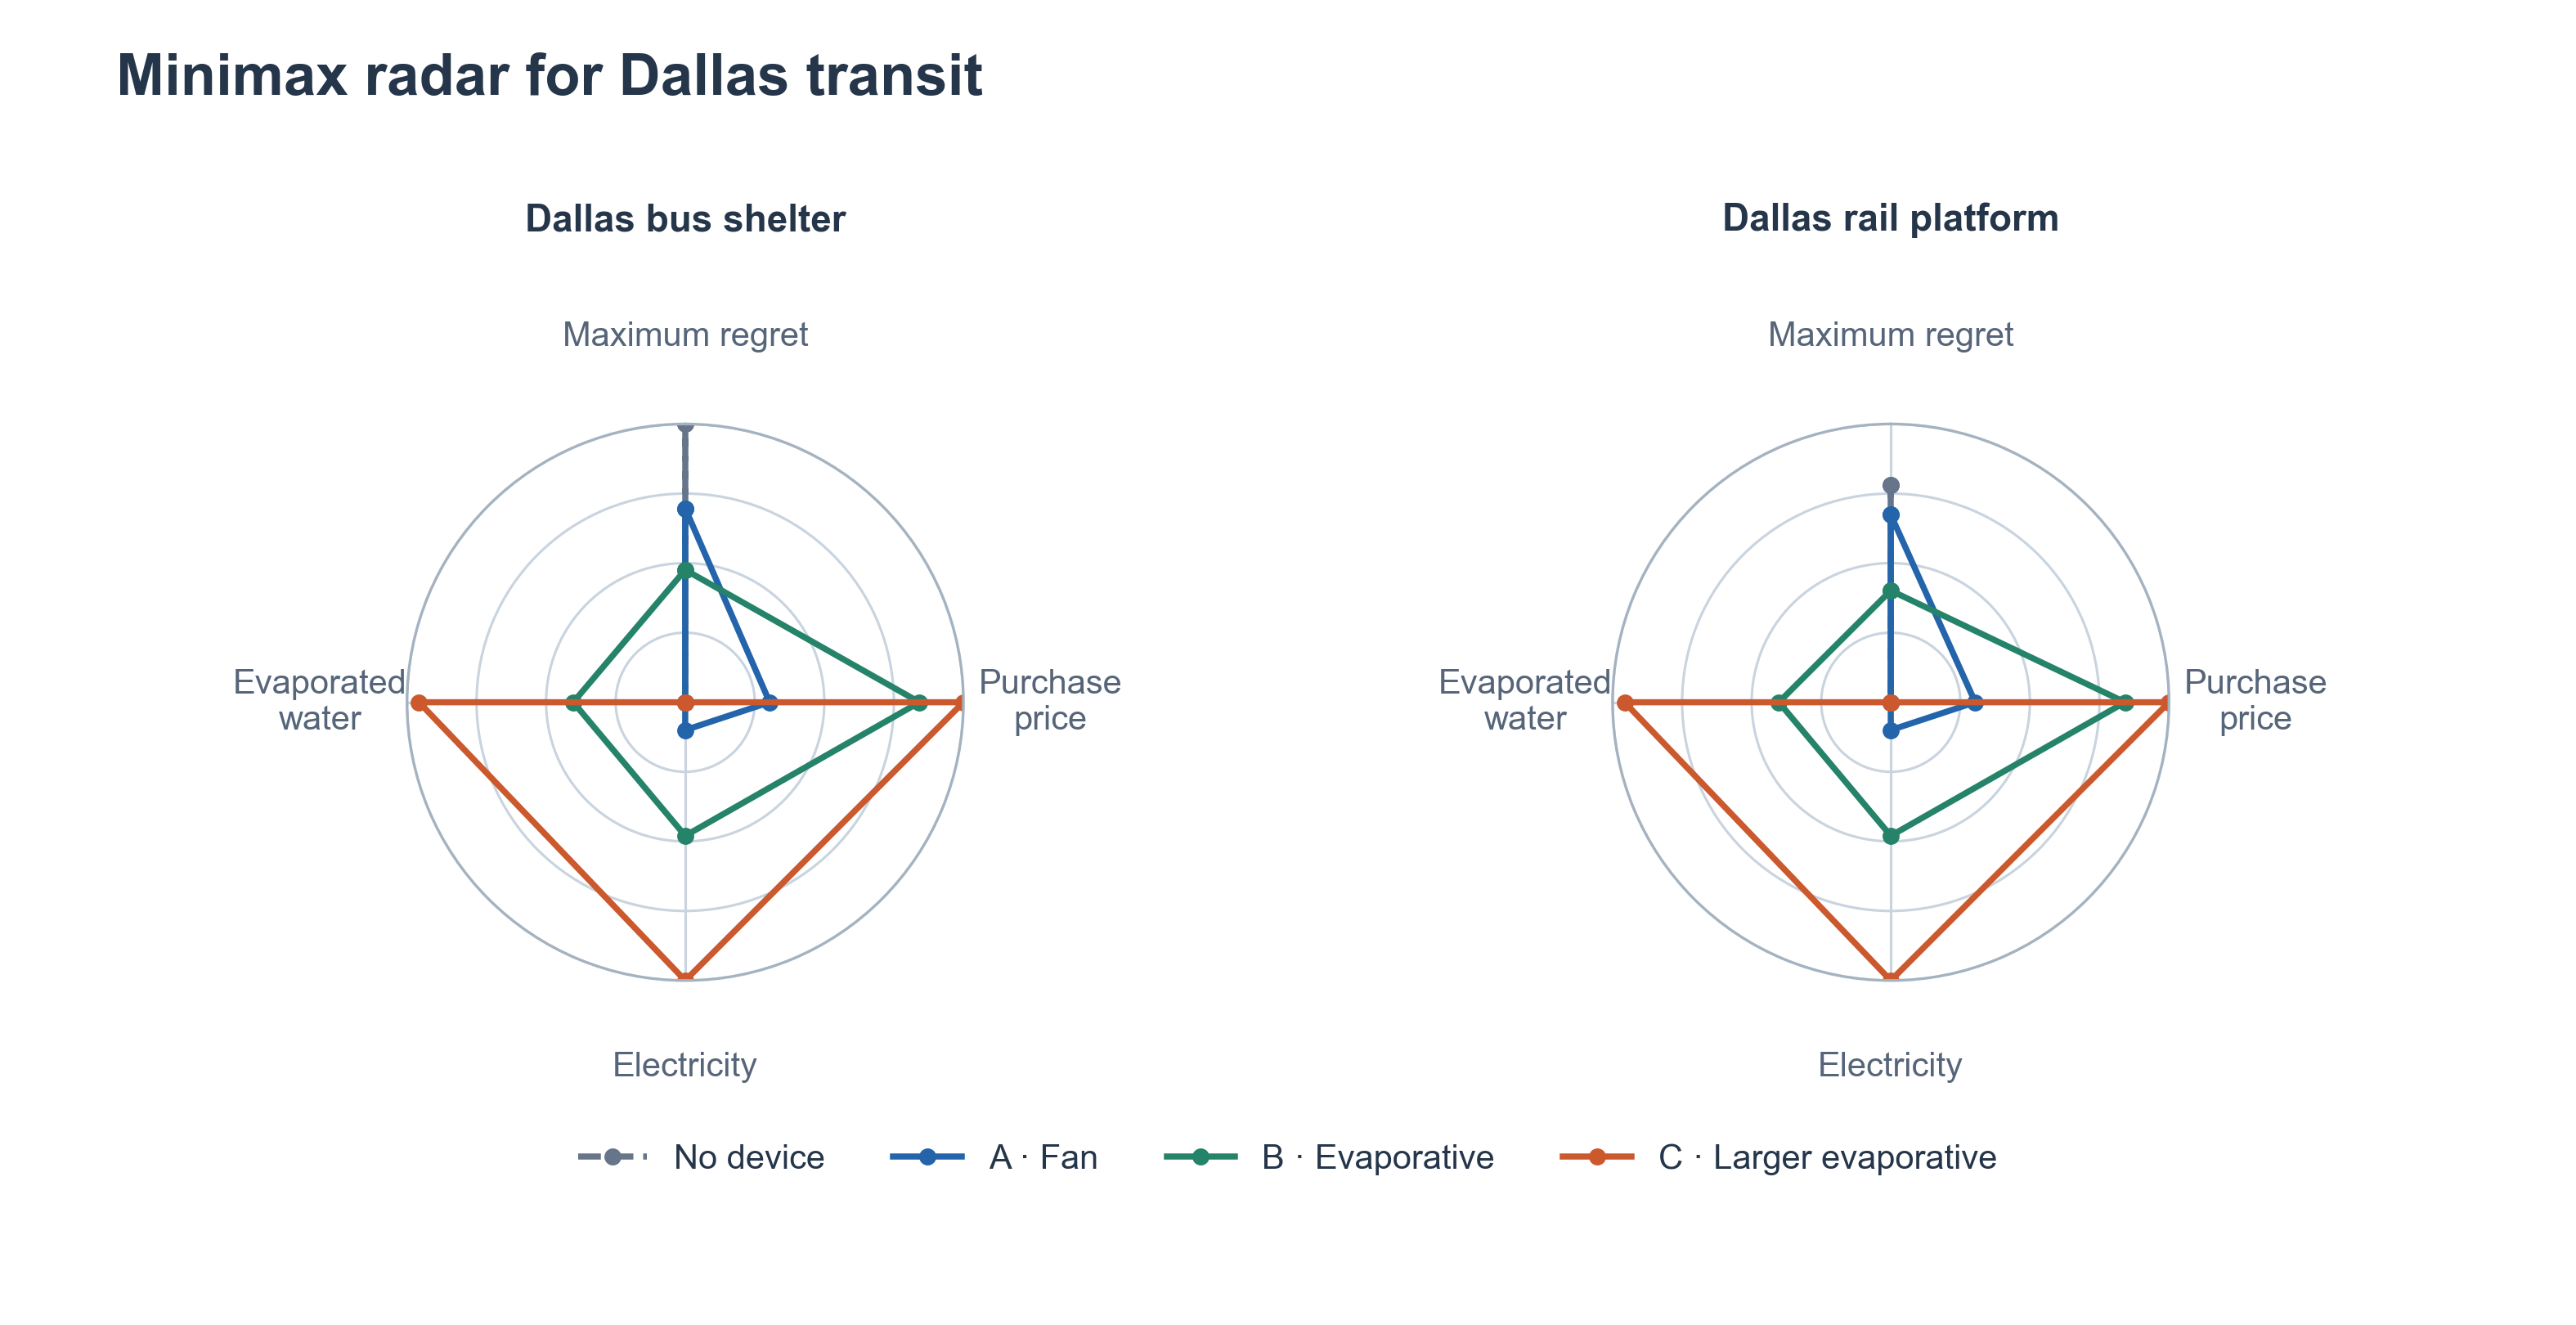
\includegraphics[width=0.94\linewidth,trim=0 0 0 51.36bp,clip]{Images/F15_dallas_transit_minimax_radar.png}
    \caption{Dallas bus shelter and rail platform radars with common scales for both venues. Minimax selection uses the maximum-regret axis.}
    \label{fig:dallas-radar}
\end{figure}

The Large Evaporative Cooler has a recorded reference purchase price of \$4,939~\cite{portacool_4000}. It draws 2.50 kWh over the modeled hour, and evaporates about 44 to 84 kg of water across the 36 modeled cases. Among bus shelters, the Small Evaporative Cooler is on the cost--regret frontier in Dallas. In Boston and Phoenix, the Fan costs less and has lower maximum regret than the Small Evaporative Cooler.

\begin{figure}[H]
    \centering
    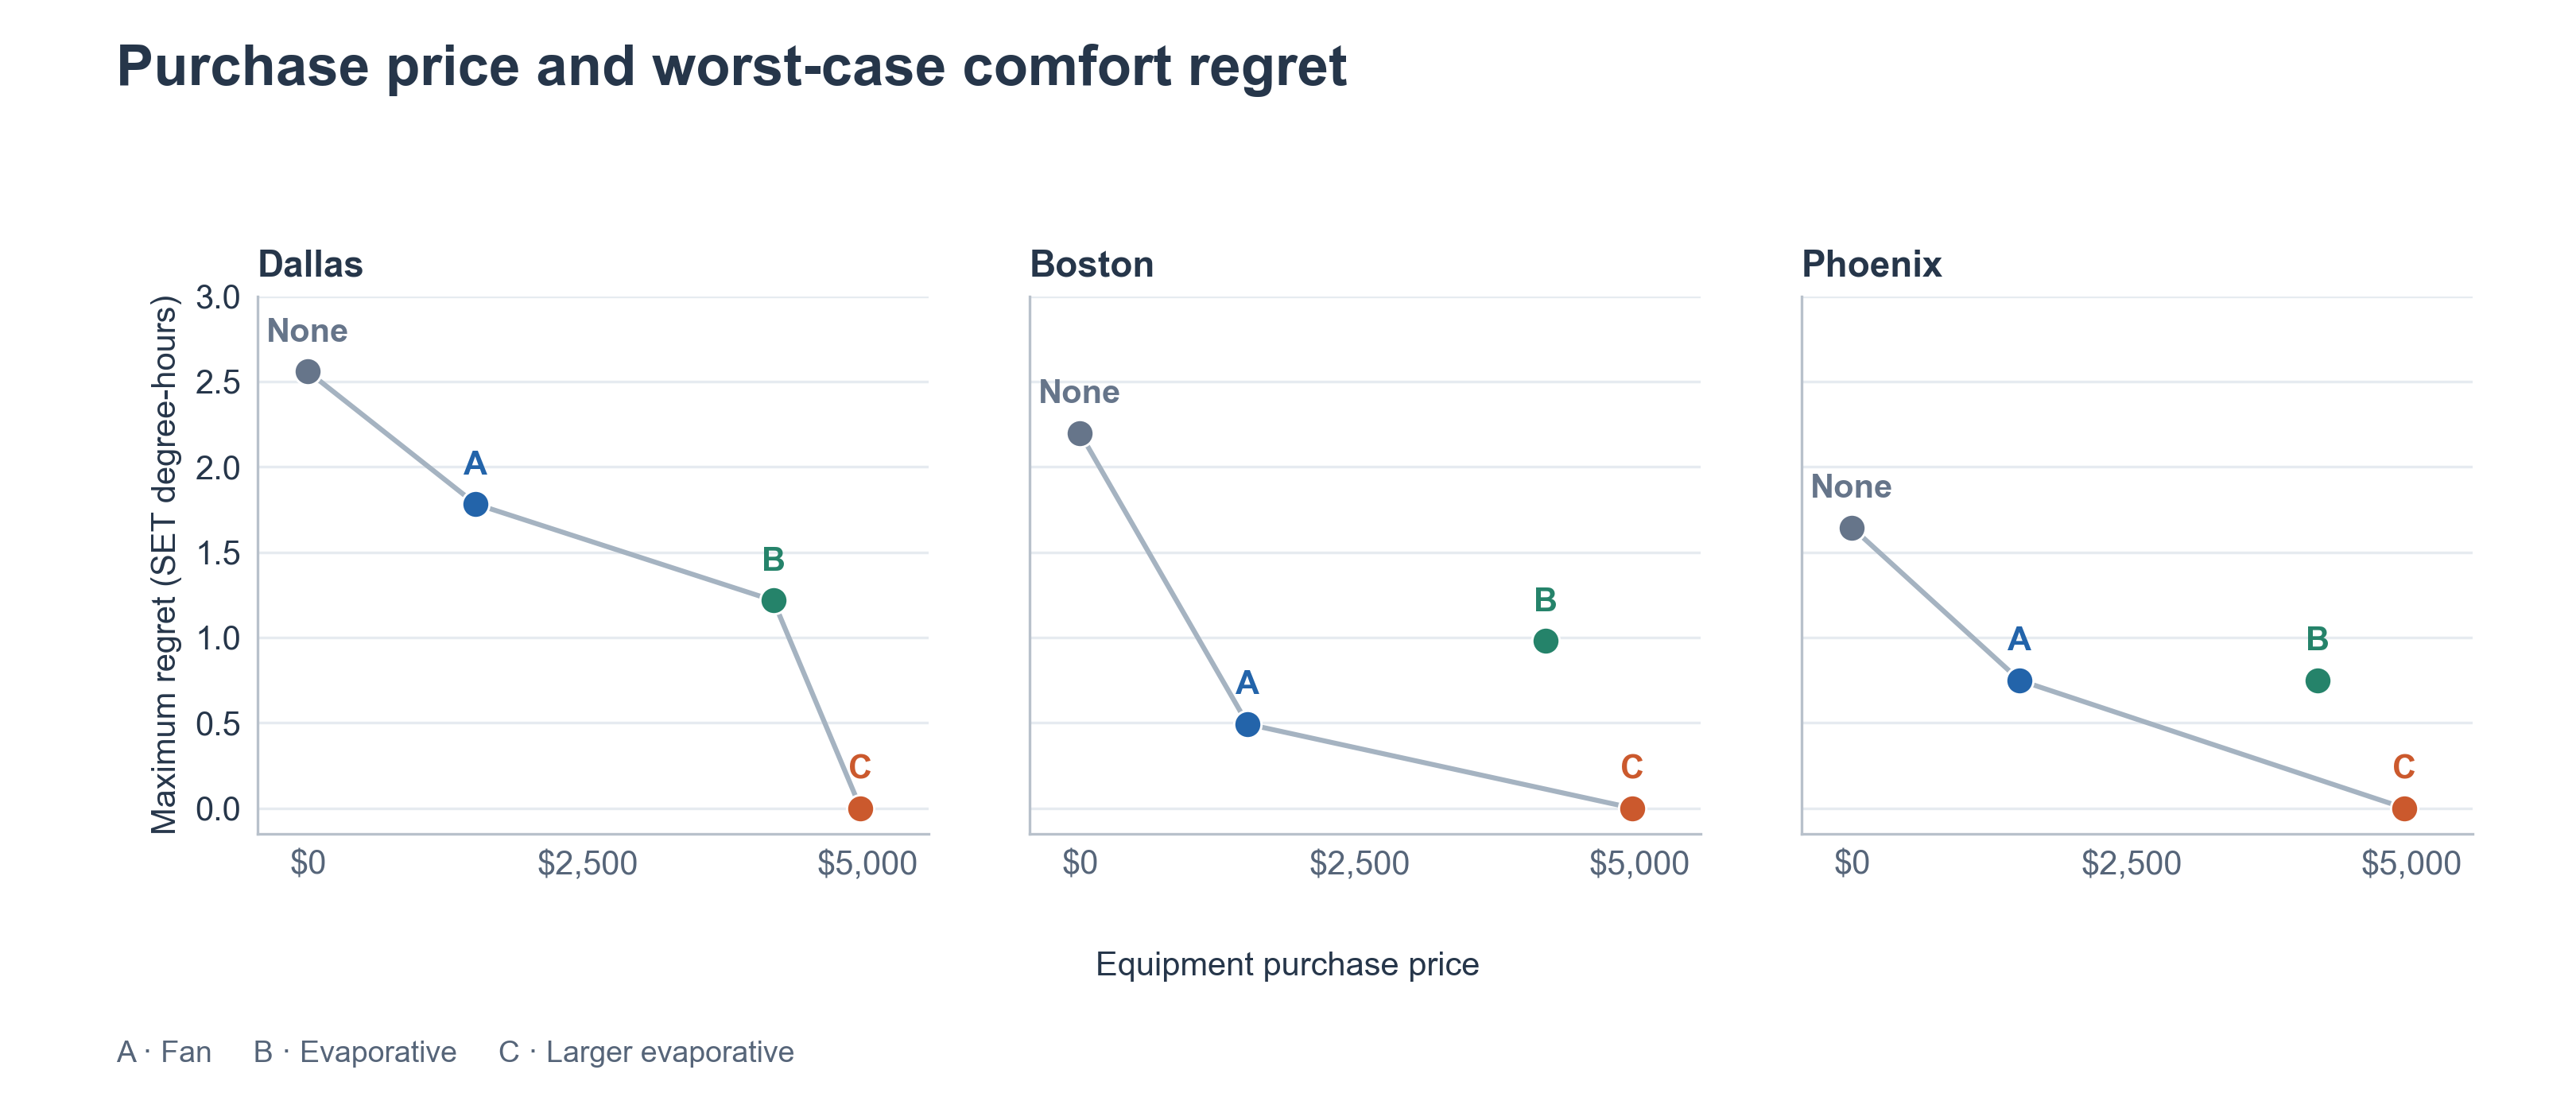
\includegraphics[width=0.92\linewidth,trim=0 0 0 68.40bp,clip]{Images/F13_bus_cost_regret_frontier.png}
    \caption{Purchase price and maximum regret at the three bus shelters. The frontier connects options for which a lower-regret choice costs more.}
    \label{fig:cost-regret}
\end{figure}

The curves also show how the value of upgrading varies across cities. In Dallas, upgrading from the Fan to the Small Evaporative Cooler costs \$2,660 and reduces maximum regret by about $0.56$ SET degree-hours. The Large Evaporative Cooler costs another \$780 and removes the remaining $1.22$ degree-hours of regret, alongside higher one-hour electricity and water use. In Phoenix, the Fan and Small Evaporative Cooler have nearly identical regret. In Boston, the Fan has lower regret and costs \$2,660 less than the Small Evaporative Cooler. These examples identify where the middle option merits a closer look and where the Fan already captures most of the attainable benefit.


\subsection{Remaining Discomfort and Sensitivity}

With the Large Evaporative Cooler, peak-hour SET ranged from 28.12\ensuremath{^{\circ}\mathrm{C}} to 33.98\ensuremath{^{\circ}\mathrm{C}} across the 12 venues. Every modeled peak-hour result remained above the 26\ensuremath{^{\circ}\mathrm{C}} comparison target.

\begin{figure}[H]
    \centering
    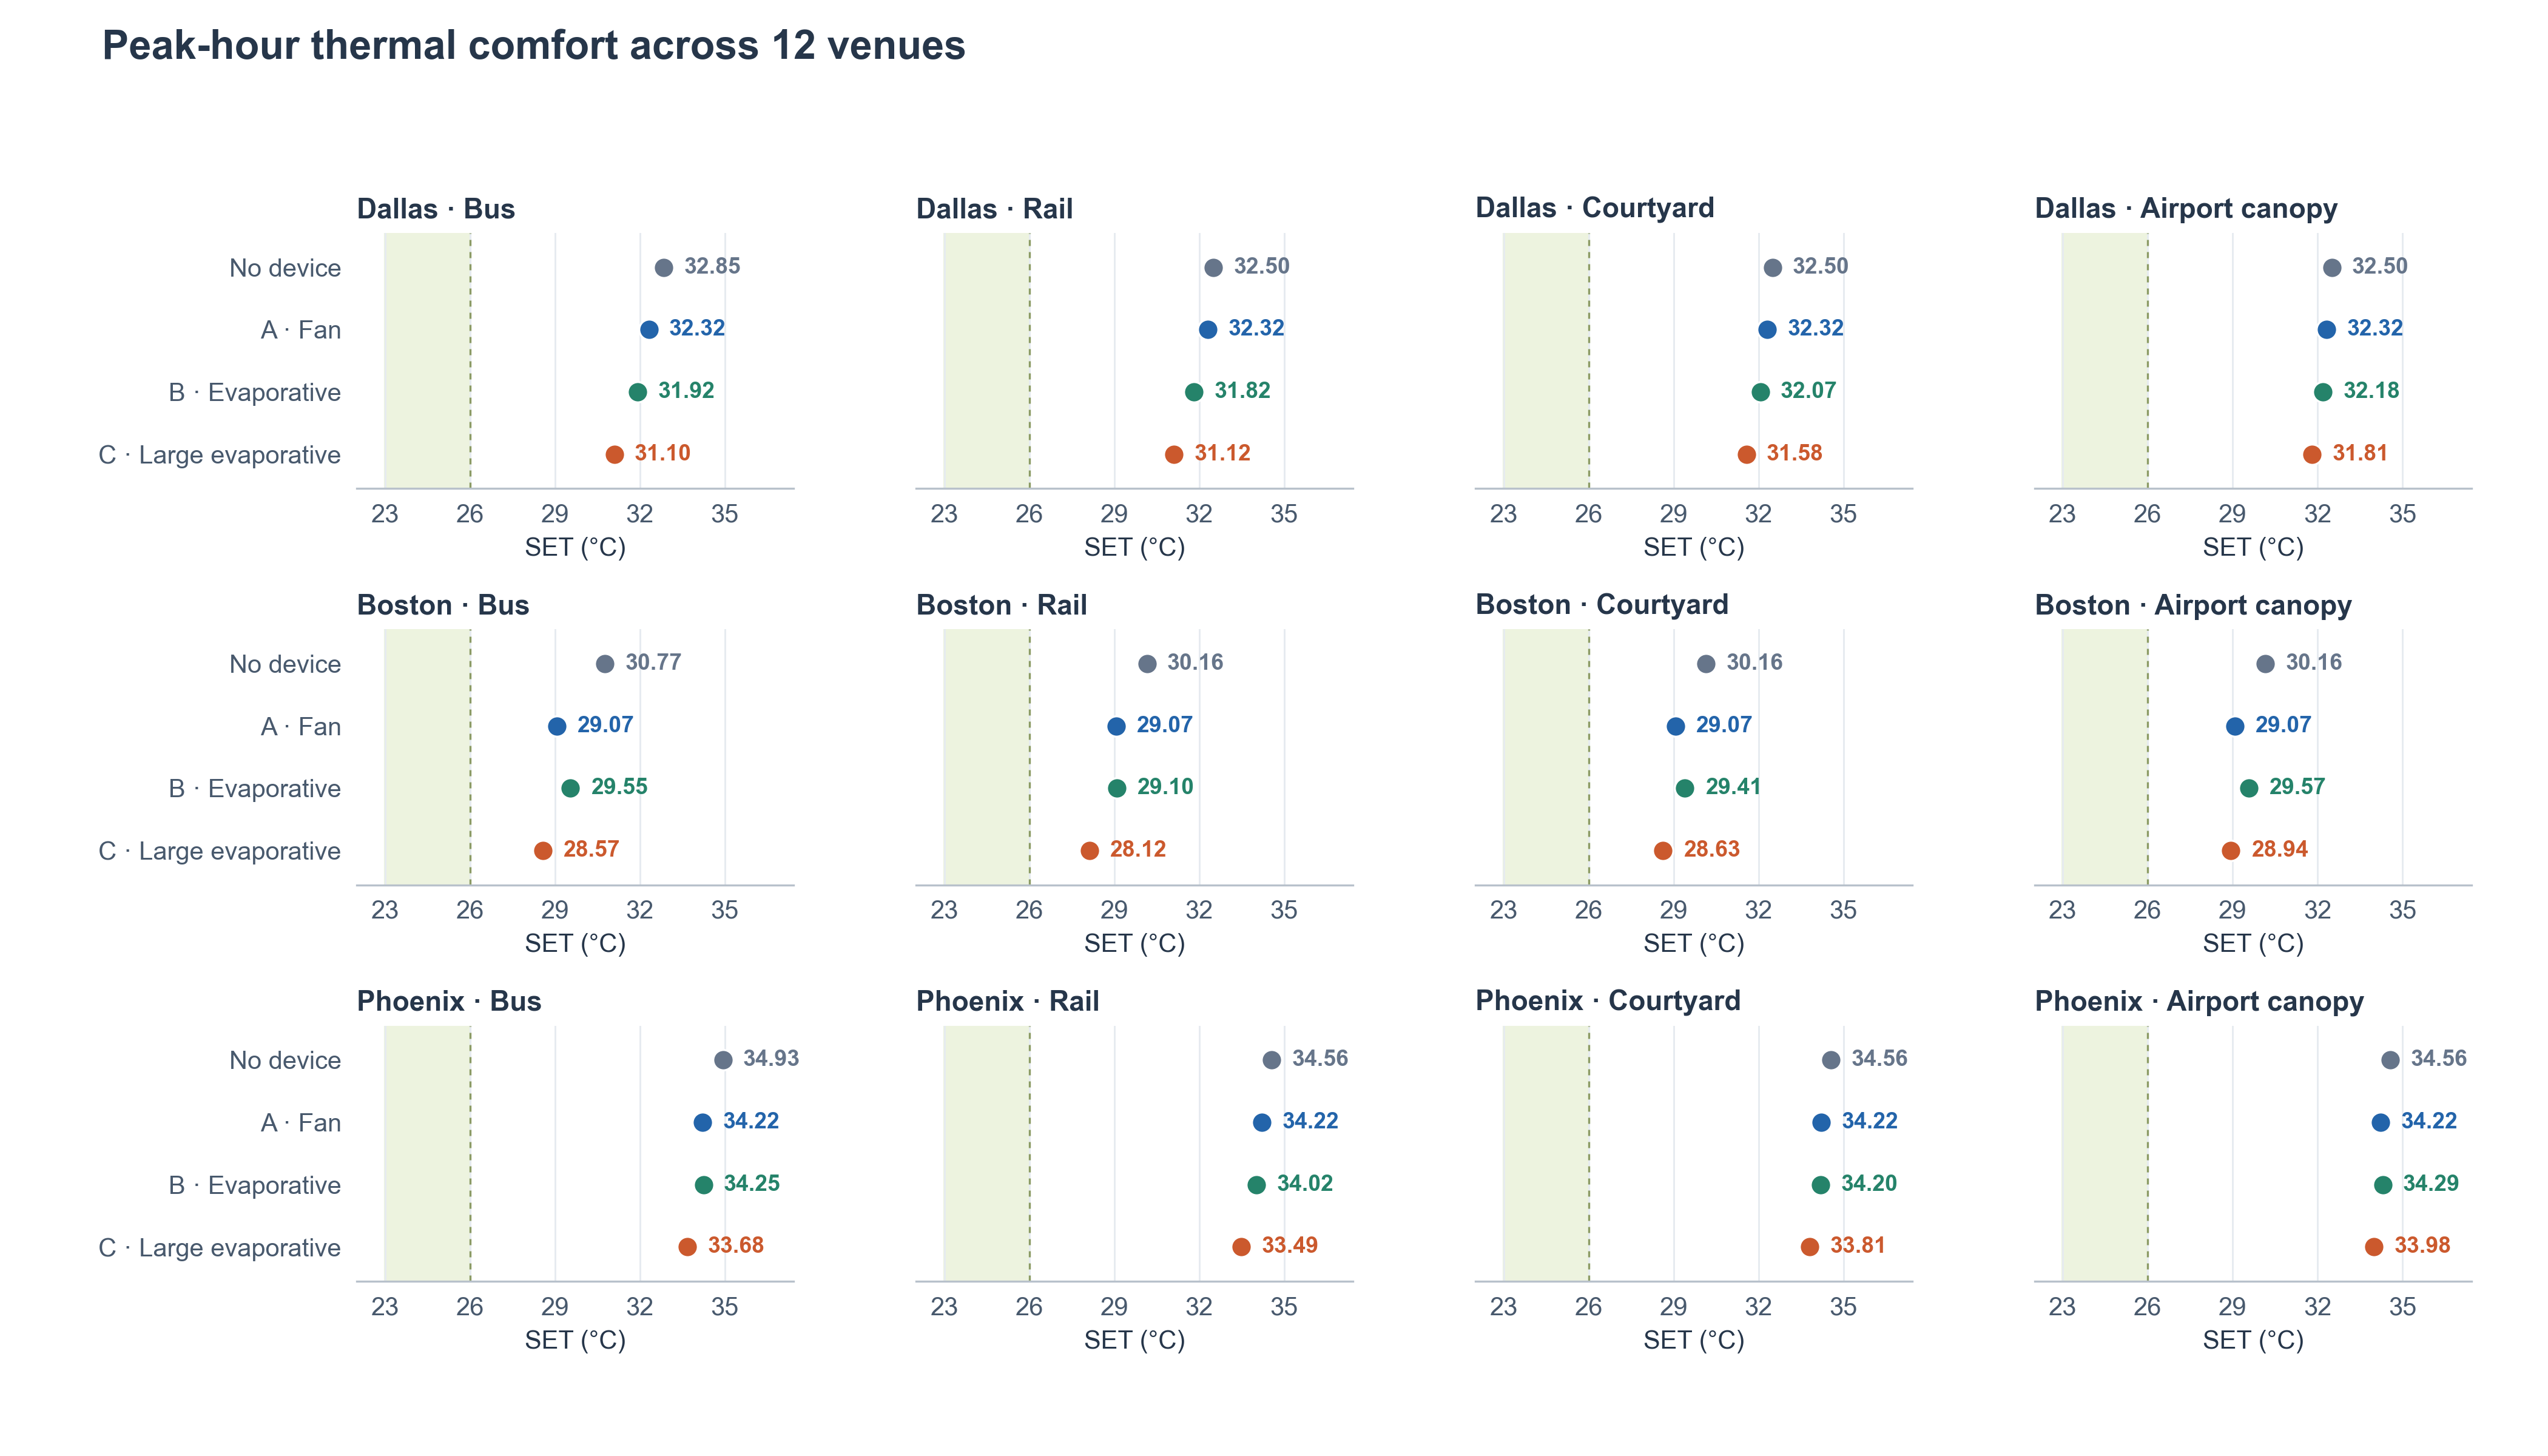
\includegraphics[width=0.95\linewidth,trim=0 0 0 69.84bp,clip]{Images/F3_all_venues_peak_comfort.png}
    \caption{Peak-hour SET at all 12 venues. The shaded band marks the 23--26\ensuremath{^{\circ}\mathrm{C}} comparison target.}
    \label{fig:peak-comfort}
\end{figure}

We varied one input at a time over five evenly spaced settings from $95\%$ to $105\%$ of its baseline in the recorded units. We tested bounded weather, airflow, equipment, exposure, and occupant inputs. The lower and upper SET thresholds were swept separately over $21.85$--$24.15\,^\circ\mathrm{C}$ and $24.70$--$27.30\,^\circ\mathrm{C}$. Other independent inputs stayed at baseline. Inflow and outflow changed together to preserve mass balance, and the radiant-temperature proxy followed outdoor temperature. We recomputed the minimax choice across the three scenarios at each setting.

\begin{figure}[H]
    \centering
    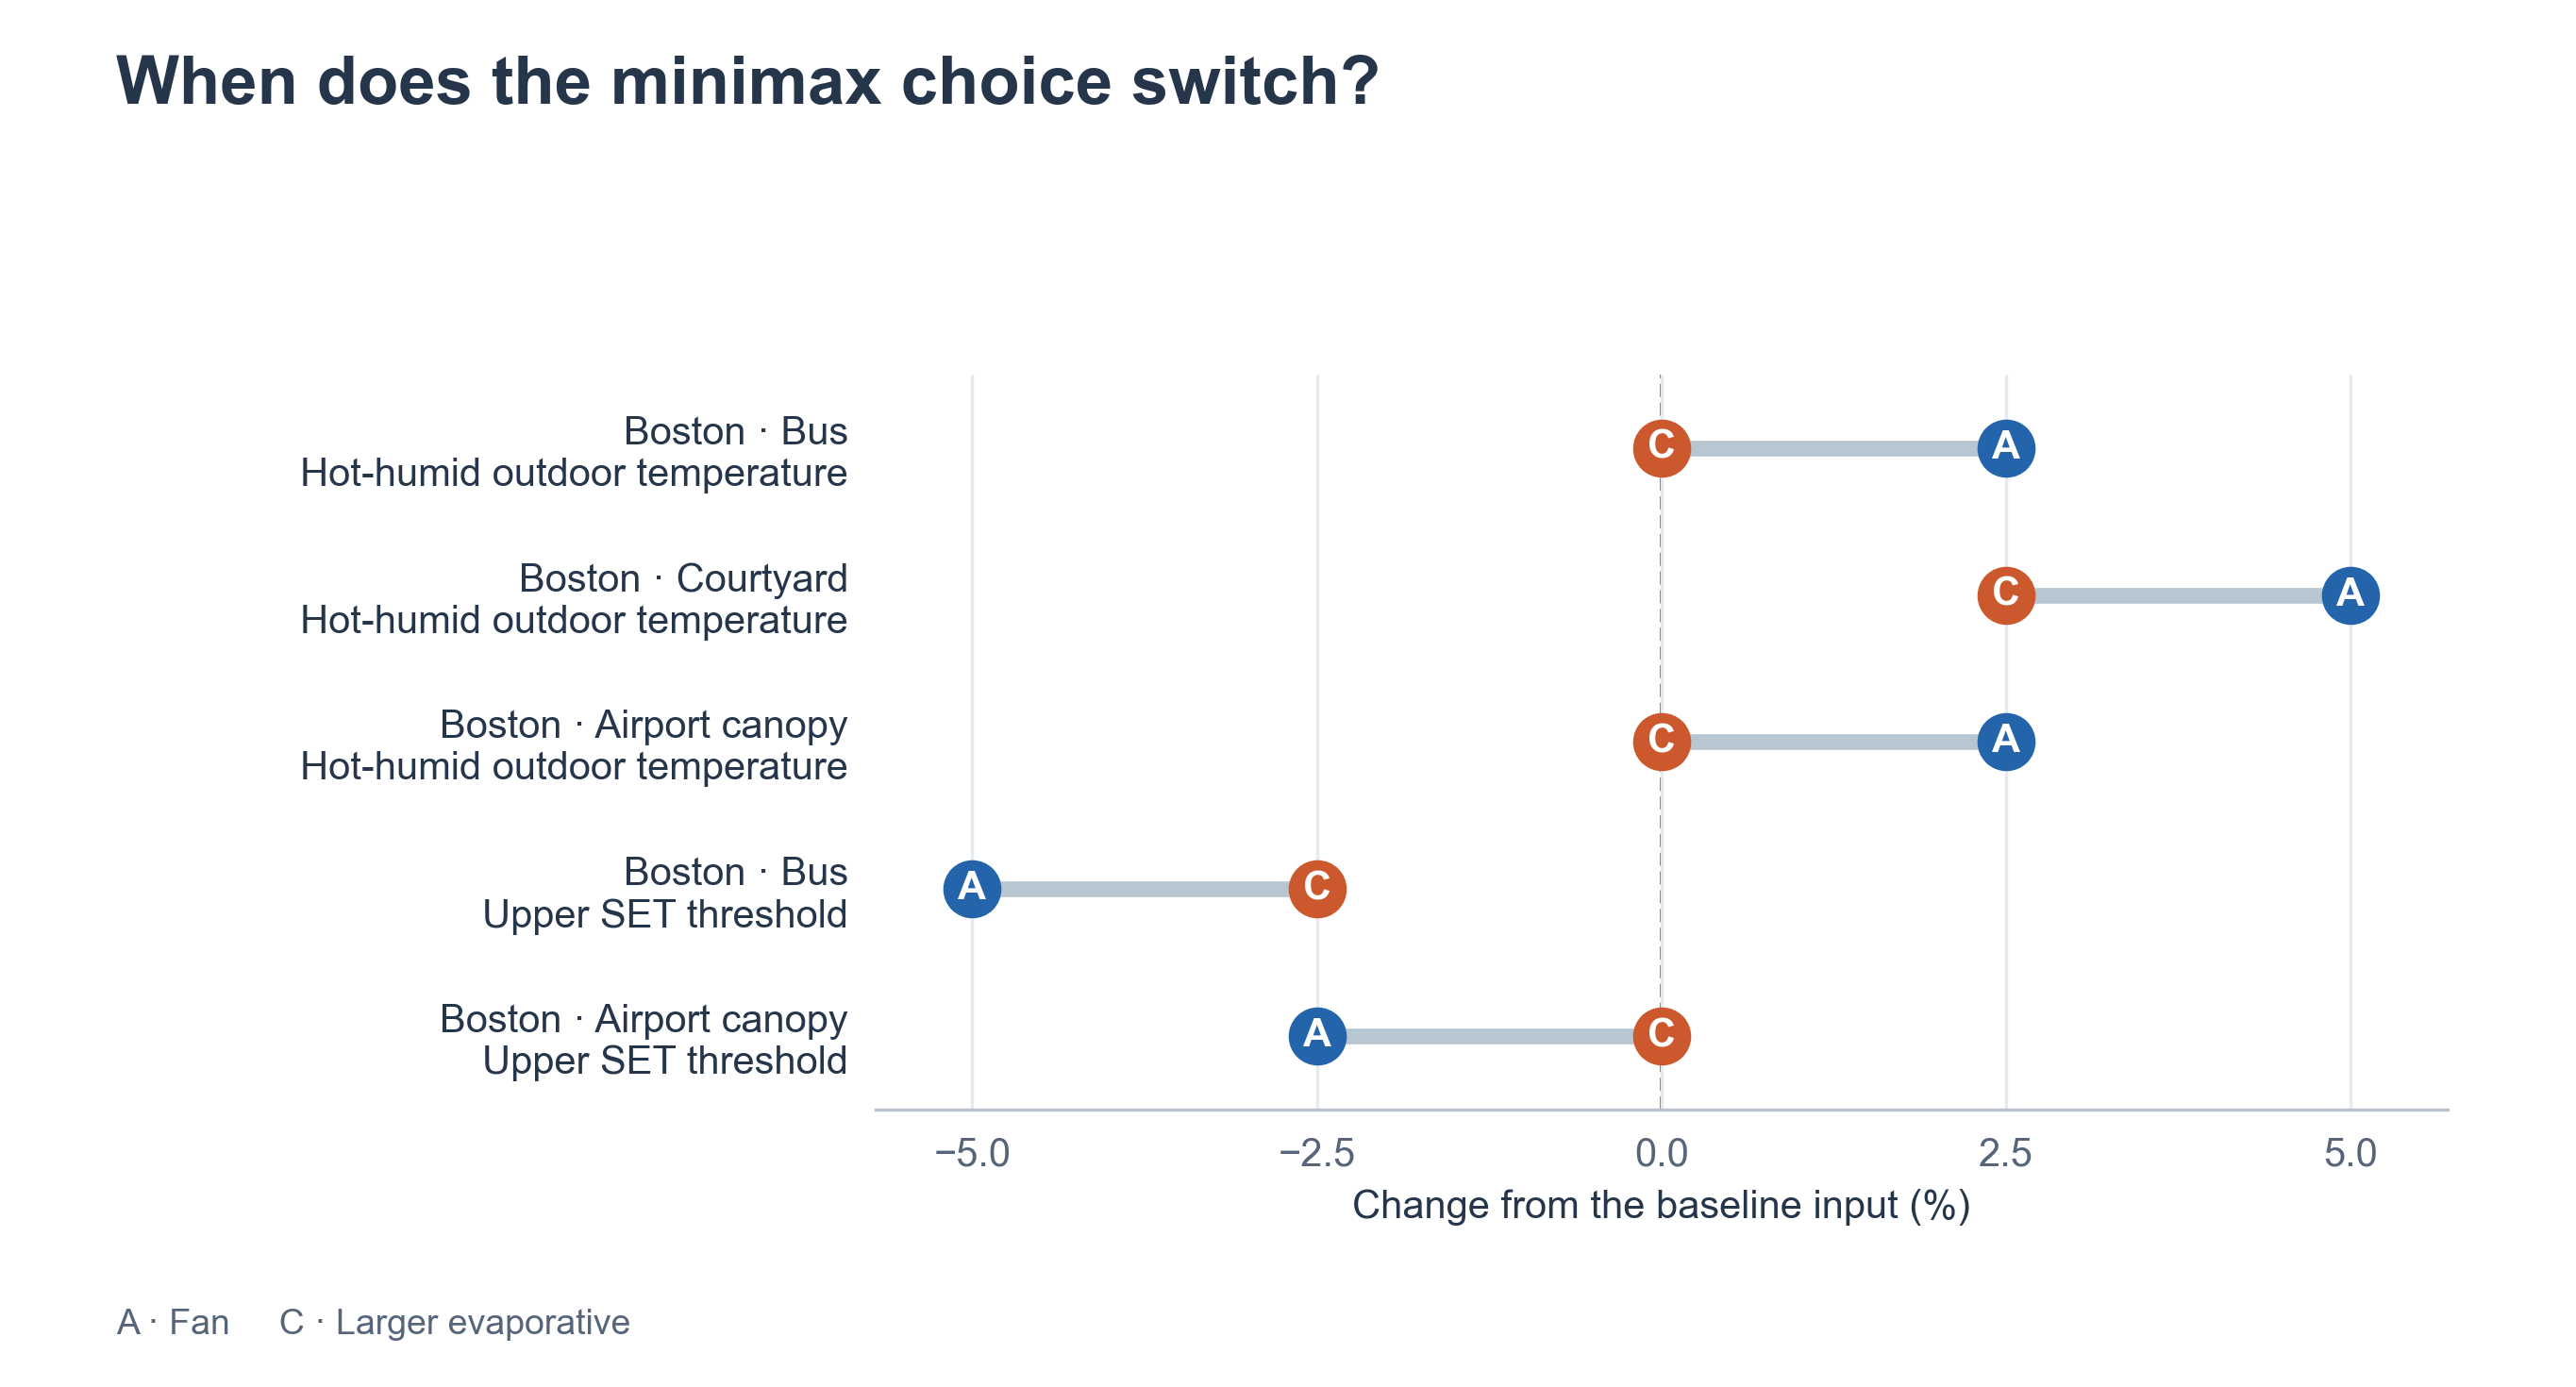
\includegraphics[width=0.78\linewidth,trim=0 0 0 94.80bp,clip]{Images/F14_minimax_sensitivity_switches.png}
    \caption{Five Boston switching intervals. Endpoints are adjacent tested settings with different minimax choices.}
    \label{fig:regret-switches}
\end{figure}

Increasing hot-humid outdoor temperature shifted the Boston choice from the Large Evaporative Cooler to the Fan between $30.39$ and $31.15\,^\circ\mathrm{C}$ at Grove Hall and the airport canopy, and between $31.15$ and $31.91\,^\circ\mathrm{C}$ at the courtyard. Raising the upper SET threshold shifted the choice from the Fan to the Large Evaporative Cooler between $24.70$ and $25.35\,^\circ\mathrm{C}$ at Grove Hall and between $25.35$ and $26.00\,^\circ\mathrm{C}$ at the airport canopy. These intervals bracket switches between sampled settings.


%% Model 3.1 %%
% \input{Subsections/Model3.1/Model3.1Method.tex}

% \input{Subsections/Model3.1/Model3.1Results.tex}

% \input{Subsections/Model3.1/Model3.1Discussion.tex}


%%%%%%%%%%%%%%%%%%%%%

\section{Model Discussion}

\subsection{Strengths}

\begin{enumerate}
    \item
    The model calculates how cooled air mixes with outdoor air before estimating the temperature in the waiting area. It also limits evaporative cooling by the outdoor wet-bulb temperature and accounts for the moisture added to the air.

    \item
    Standard Effective Temperature combines air temperature, humidity, airspeed, and radiant temperature into a common comfort measure. This allows the model to capture the benefit of a fan even when it leaves the air temperature unchanged.

    \item
    We report SET reduction per kWh separately from hot-discomfort loss and minimax regret.

    \item
    Minimax regret ranks equipment at each venue by its largest regret across three hot-weather scenarios. At Grove Hall, we tested how limits on purchase cost, electricity, and water changed the selection.

    \item
    The sensitivity sweeps locate intervals where the recommendation changes as individual inputs vary.
\end{enumerate}

\subsection{Weaknesses}

\begin{enumerate}
    \item
    The model estimates average conditions in each waiting area. This keeps the comparison consistent across venues, although cooling at a particular seat may differ from the zone average.

    \item
    We use the uncooled outdoor air temperature as a proxy for mean radiant temperature. Passenger-level measurements could assess how shade and hot surfaces affect this approximation.

    \item
    Each venue has three modeled weather cases. Different weather or resource limits could change the ranking. The sweeps consider individual inputs, so joint effects remain uncertain.
\end{enumerate}

\section{Conclusion}

\indent We studied how cooling devices reduce passenger discomfort in outdoor and semi-outdoor waiting areas. We estimated how much cooling reaches passengers, how much relief it provides, and which option performs best across the modeled weather conditions. We compared a fan and two evaporative coolers with a no-device baseline at 12 venues.

\indent In Model I, we found that the cooling at the outlet of an evaporative cooler is greater than the cooling in the waiting area after the air mixes. The amount of cooling available also depends on outdoor humidity. Model II used Standard Effective Temperature (SET) to compare how the devices feel to a passenger and how much discomfort each device reduces per kilowatt-hour. In Model III, the Large Evaporative Cooler led the comfort benchmark. The Fan led the minimax comparison for Grove Hall under the illustrative purchase, electricity, and water limits. Even with the Large Evaporative Cooler, peak-hour SET ranged from $28.12$ to $33.98\,^\circ\mathrm{C}$ and stayed above the $26\,^\circ\mathrm{C}$ comparison target at all 12 venues. Sensitivity analysis found five intervals where a Boston recommendation switched between the Fan and the Large Evaporative Cooler. In three of those intervals, increasing the outdoor temperature in the hot-humid scenario favored the Fan.

\indent The operating rule uses the $23$--$26\,^\circ\mathrm{C}$ band to decide when equipment can stay off. The equipment ranking uses hot-discomfort loss above the upper threshold.

\indent The modeled cases below show how hot-discomfort loss and available resources guide the operating choice.

\begin{table}[H]
  \centering
  \renewcommand{\arraystretch}{1.3}
  \begin{tabularx}{\textwidth}{>{\raggedright\arraybackslash}p{0.18\textwidth}Yp{0.48\textwidth}}
    \toprule
    \textbf{Option} & \textbf{When to use it} & \textbf{Evidence from the model} \\
    \midrule
    No cooling & The waiting area already meets the comfort target. & At Grove Hall in the hot-dry case, baseline SET is $24.44\,^{\circ}\mathrm{C}$, within the $23$--$26\,^{\circ}\mathrm{C}$ band. \\
    \rowcolor{gray!15}
    Fan & The Fan provides enough relief or cooling per kWh is the priority. & At Grove Hall in the hot-humid case, the Fan reduces SET from $27.66$ to $25.09\,^{\circ}\mathrm{C}$ using $0.25$ kWh and no water. \\
    Small Evaporative Cooler & Extra relief is needed and resources limit the choice. & At the Dallas bus shelter in peak heat, this cooler reduces SET by $0.40\,^{\circ}\mathrm{C}$ beyond the Fan, using an extra $0.95$ kWh and about $33$ kg of water. SET still exceeds the comfort target. \\
    \rowcolor{gray!15}
    Large Evaporative Cooler & Reducing remaining hot discomfort is the priority, and electricity and water are available. & This cooler leads the comfort benchmark at all 12 venues. At the Dallas bus shelter in peak heat, it improves on the Small Evaporative Cooler by $0.82\,^{\circ}\mathrm{C}$ SET using an extra $1.30$ kWh and about $45$ kg of water. \\
    \bottomrule
  \end{tabularx}
\end{table}

\indent The Grove Hall peak-hour comparison in Figure~\ref{fig:grove-hall-peak-tradeoff} shows why the operating choice depends on the value of the last increment of cooling. The Fan avoids $1.71$ SET degree-hours of hot discomfort using $0.25$ kWh. The Small Evaporative Cooler uses $1.20$ kWh and avoids only $1.22$ degree-hours, so the Fan outperforms it on both measures in this case. The Large Evaporative Cooler avoids $2.20$ degree-hours. Switching from the Fan to the Large Evaporative Cooler therefore buys about $0.49$ additional degree-hours of relief for $2.25$ extra kWh, and the modeled SET still exceeds the comfort target.

\begin{figure}[H]
    \centering
    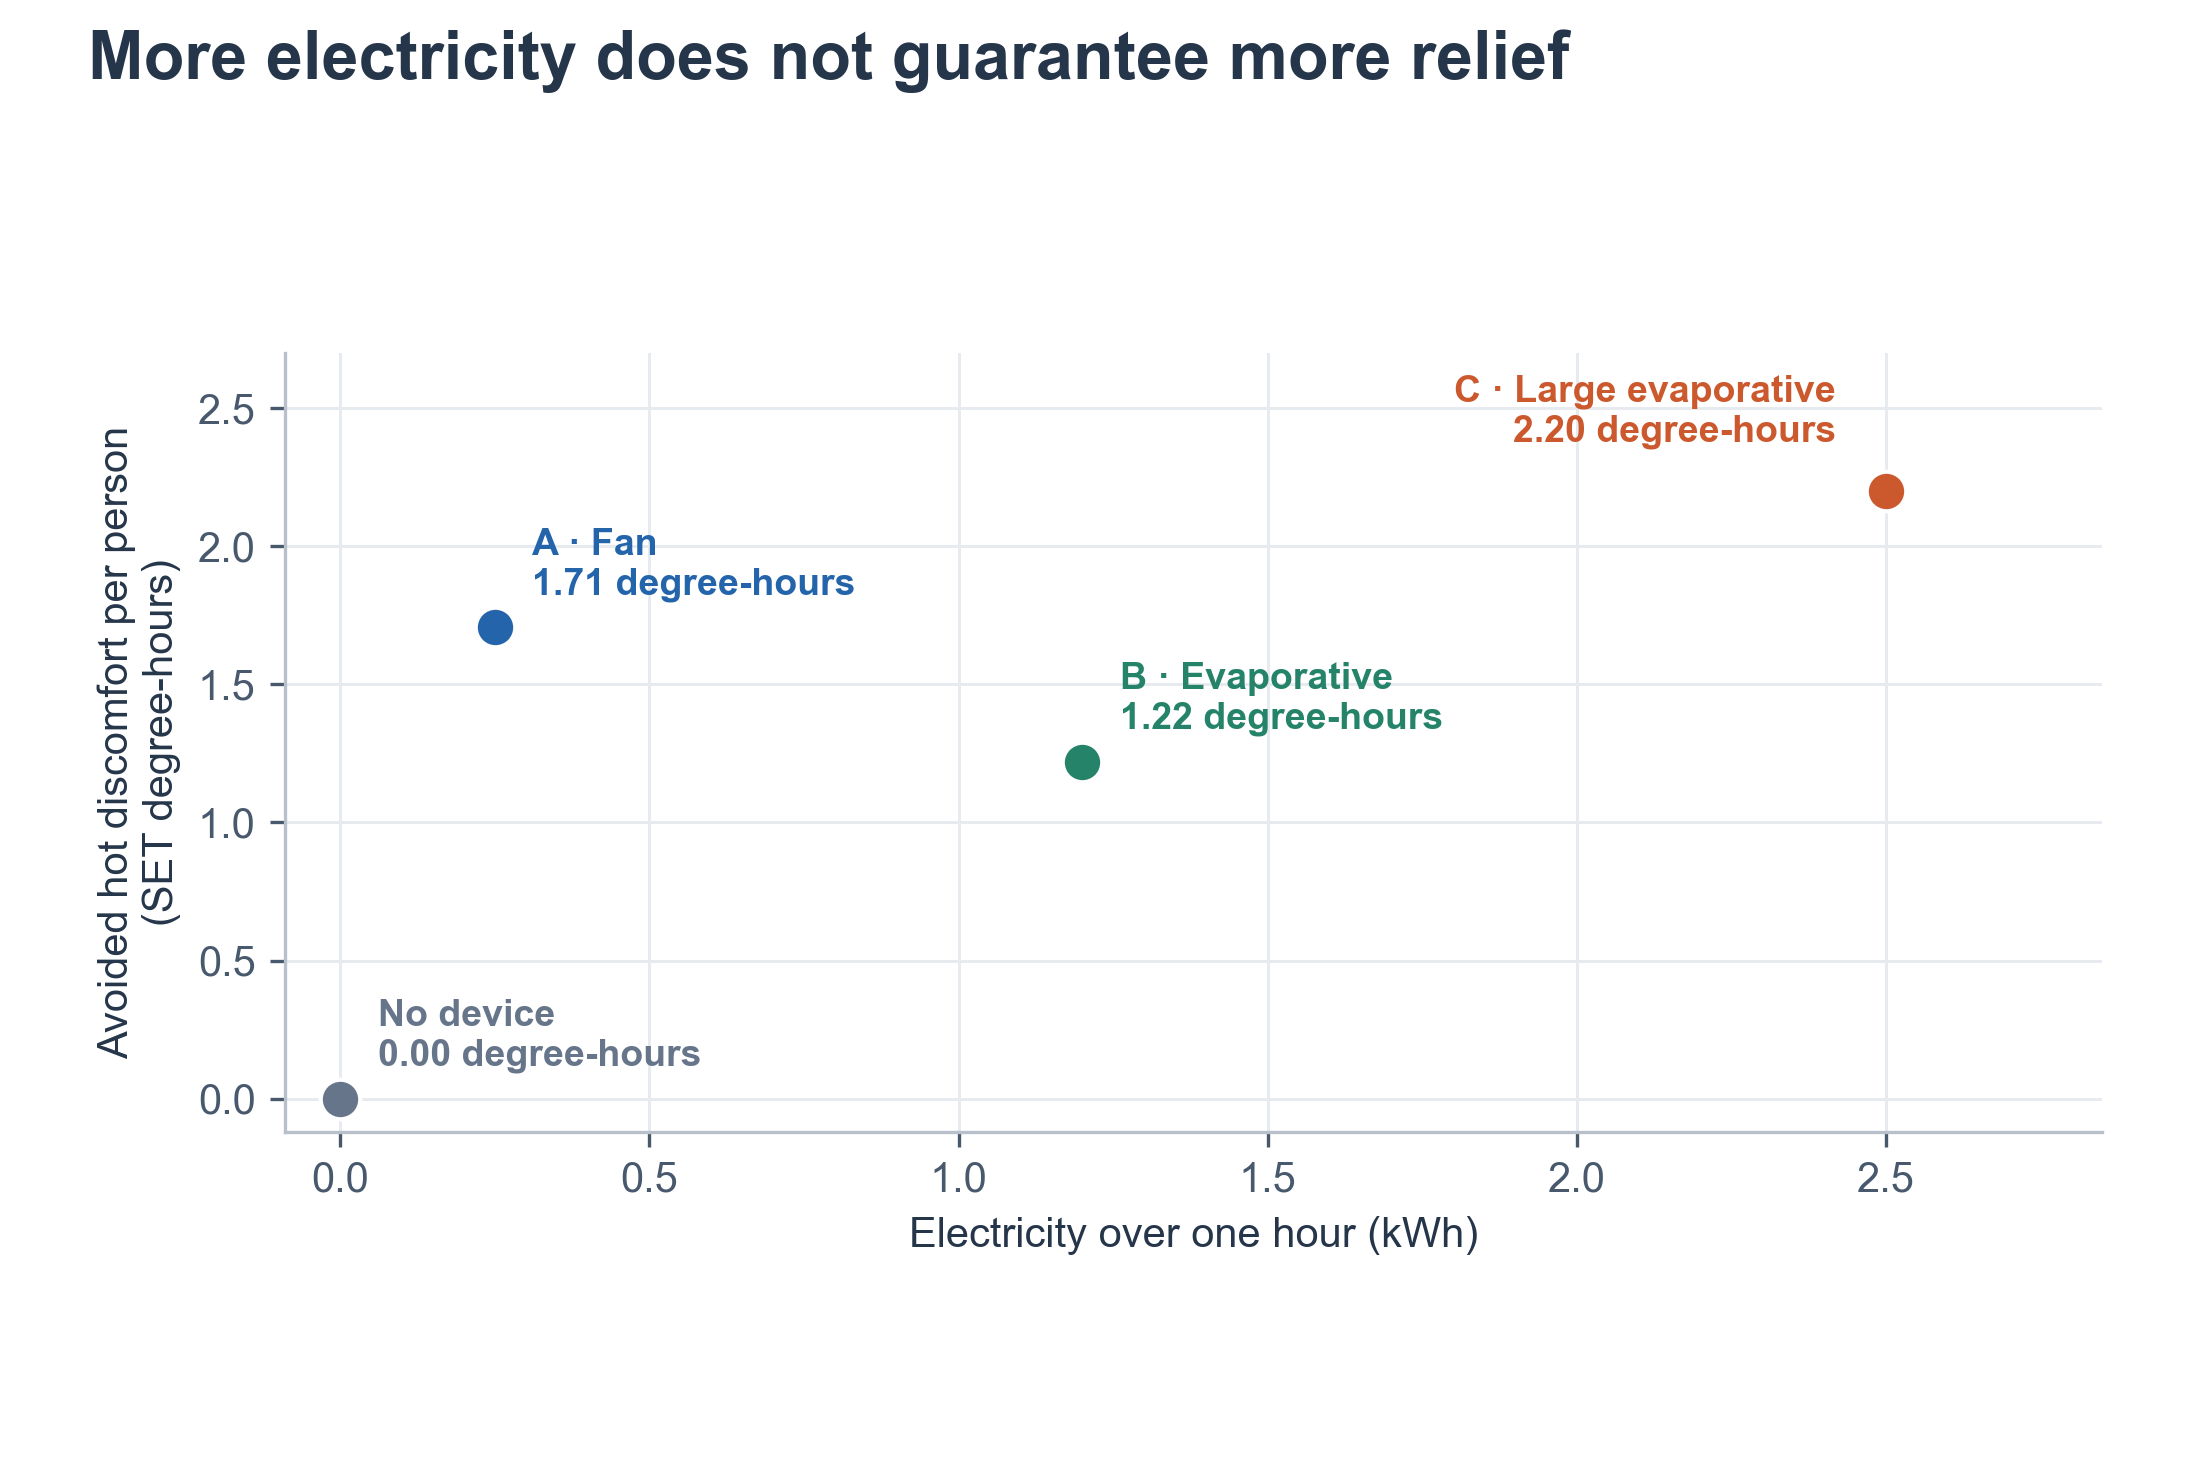
\includegraphics[width=0.66\linewidth,trim=0 0 0 76.32bp,clip]{Images/F2_boston_benefit_electricity.png}
    \caption{Electricity use and avoided hot discomfort at the Grove Hall bus shelter during the modeled peak-temperature hour.}
    \label{fig:grove-hall-peak-tradeoff}
\end{figure}

\indent Before installing equipment permanently, we recommend a pilot at Grove Hall. During humid heat and peak heat, measure air temperature, humidity, airspeed, and mean radiant temperature where passengers sit and stand. Compare the Fan and Large Evaporative Cooler at the same passenger positions, and test added shade during the peak period. The measurements would show where the Fan provides enough relief and whether shade helps close the gap to the comfort target.

\indent Across all 12 venues, we recommend the Large Evaporative Cooler when minimizing worst-case regret in hot-discomfort loss is the priority and the venue can meet its purchase, electricity, and water requirements. To identify fallback options, we recomputed regret with the Large Evaporative Cooler excluded and the remaining options feasible. In \textbf{Dallas}, choose the Small Evaporative Cooler at the bus shelter, rail platform, courtyard, and airport canopy when its resource requirements can be met. In \textbf{Boston}, choose the Fan at the bus shelter, rail platform, courtyard, and airport canopy. In \textbf{Phoenix}, choose the Small Evaporative Cooler at the rail platform and the Fan at the airport canopy. At the Phoenix bus shelter and courtyard, we recommend the Fan for its lower cost and water-free operation. The Small Evaporative Cooler has slightly lower maximum regret at those two sites, by less than $0.07$ SET degree-hours in each case. If water is unavailable for either cooler, use the Fan when cooling is needed and leave equipment off when the waiting area already meets the comfort target.


\newpage
\section{Memorandum to the Chief Operations Officer of HiMCM}

\noindent\textbf{To:} Chief Operations Officer, HiMCM\\
\textbf{From:} Team 19678\\
\textbf{Date:} November 16, 2026\\
\textbf{Subject:} Cooling strategy for the Grove Hall bus shelter

We recommend the Fan as Grove Hall's primary cooling system. Consider the Large Evaporative Cooler for peak heat if resources allow. In the humid summer conditions we modeled, the Fan brought passengers within our comfort range using no water and just 0.25 kWh of electricity in one hour. In Boston's hot-dry case, the shelter was already comfortable with the equipment off. The Large Evaporative Cooler provided additional relief during the peak-heat case.

Grove Hall was one of six bus and rail waiting areas in our broader study of 12 sites across Boston, Dallas, and Phoenix. Using summer 2025 weather data, we compared a fan, two sizes of evaporative cooler, and no cooling. At an open-sided shelter, passenger comfort depends on air temperature, humidity, and airflow. A fan moves air across the skin. An evaporative cooler lowers the air temperature and adds humidity as the supply air mixes with outdoor air. To compare what passengers would experience, we used Standard Effective Temperature (SET), which expresses the combined effects of temperature, humidity, airflow, and radiant heat on a common temperature scale. The figures below are estimates on that scale. We used 23--26$^{\circ}$C as our comfort range.

In the hot-humid case, the Fan brought estimated conditions from 27.66$^{\circ}$C to 25.09$^{\circ}$C. All three devices reached the target. The Fan used 90\% less electricity than the Large Evaporative Cooler and saved about 44 liters of water in the modeled hour. It also had the lowest reference purchase price at \$1,499, compared with \$4,159 for the Small Evaporative Cooler and \$4,939 for the Large Evaporative Cooler~\cite{aireye_20_price,portacool_2000,portacool_4000}. In the hot-dry case, the shelter started at 24.44$^{\circ}$C, and all three devices pushed conditions below the lower end of the comfort range.

Peak heat presented a harder decision. With the equipment off, estimated conditions reached 30.77$^{\circ}$C. The Fan brought that down to 29.07$^{\circ}$C and the Large Evaporative Cooler to 28.57$^{\circ}$C. The Large Evaporative Cooler led the comfort benchmark. When we tested limits on purchase cost, electricity, and water at Grove Hall, the Fan was the best feasible option across the three scenarios. The practical trade-off is what it took to gain that last half-degree during the peak hour: 2.50 kWh of electricity, ten times the Fan's consumption, and roughly 81 liters of evaporated water. Even then, conditions remained above the comfort target.

\medskip
\noindent\textbf{Key Recommendations}
\begin{enumerate}
\setlength{\itemsep}{2pt}
\setlength{\parsep}{0pt}
\item \textbf{Leave cooling off when the shelter is already comfortable.} In Boston's hot-dry scenario, the uncooled waiting area was within the target range, and all three systems would have cooled it below that range. Under those conditions, operators can save electricity and water simply by leaving the equipment off.
\item \textbf{Use the Fan as Grove Hall's primary source of relief.} In humid heat, the Fan brought passengers within the comfort range using 90\% less electricity than the Large Evaporative Cooler and no water. As long as the Fan meets that target, there is little reason to run either evaporative cooler.
\item \textbf{Consider the Large Evaporative Cooler for peak heat if resources allow.} The Large Evaporative Cooler provided about half a degree of extra relief at peak heat. Across the modeled hours, it requires \$4,939 upfront, 2.50 kWh per hour, and a water allowance of about 84.1 liters for the highest-use hour.
\item \textbf{Provide access to air-conditioned shelter during hazardous heat.} Even with the Large Evaporative Cooler running, Grove Hall remained above the comfort target during peak heat. Identify a nearby air-conditioned place where passengers can wait and post clear directions at the stop.
\end{enumerate}

\clearpage
\phantomsection
\addcontentsline{toc}{section}{Public Blog Post}
\begin{figure}[H]
    \centering
    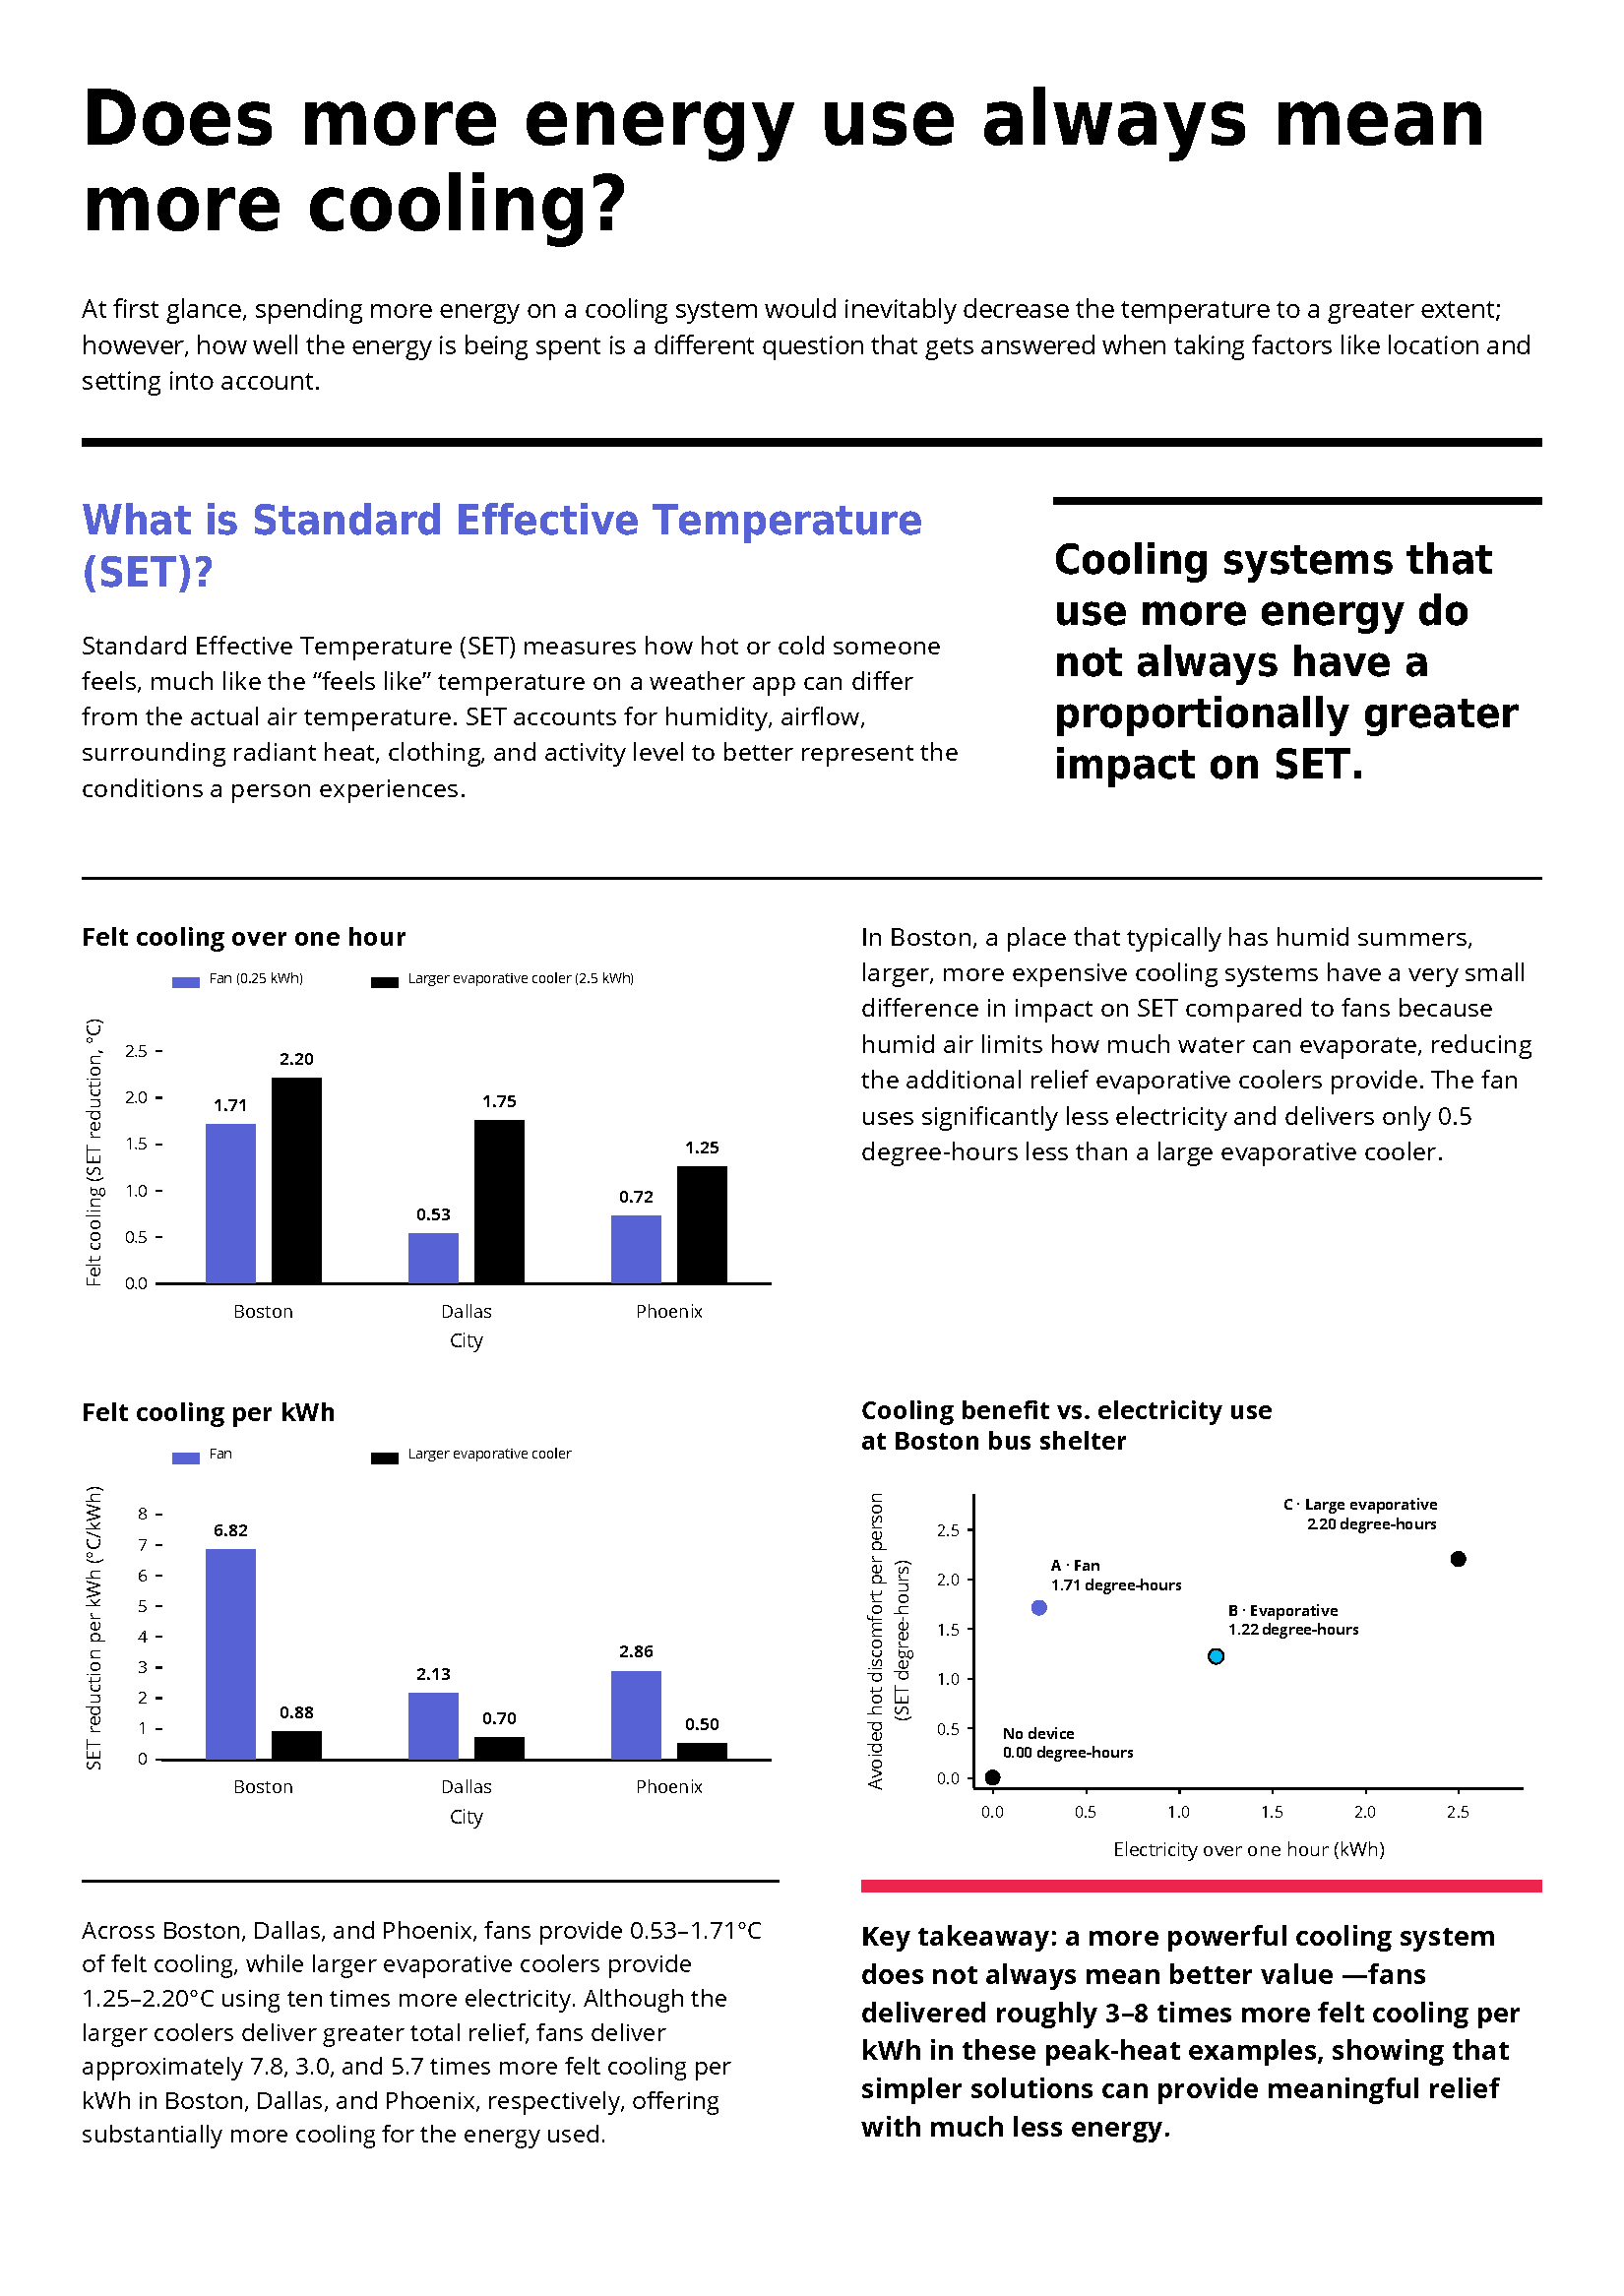
\includegraphics[width=0.88\linewidth]{Images/HiMCM26_BlogPost_Designed.pdf}
    \label{fig:blog-post}
\end{figure}

\newpage
\bibliographystyle{abbrv}

{\small
\bibliography{HiMCM}
}

\clearpage
\appendix
\setcounter{secnumdepth}{-1}
\phantomsection
\section{Appendix A: Project Repository}

\noindent We document our data and models in the HiMCM26 GitHub repository.

\noindent\url{https://github.com/LordVanra/HiMCM26}

\clearpage
\phantomsection
\section{Report on Use of AI Tools}
{\raggedright

\subsection*{Prompt 1}
Find simultaneous summer 2025 weather data for Dallas that can supply outdoor temperature, relative humidity, and pressure to our heat and moisture inputs. Don’t make up any data or fill gaps with typical values. Give me the original source, the exact page, table, or variable to look for, and a link with steps to download it. Keep measurements, published specifications, derived inputs, and project assumptions clearly labeled. If you can’t verify something, leave it missing and tell me what is still needed. Only find and document data; don’t run the cooling models.

\needspace{4\baselineskip}
\subsubsection*{AI output}
Use the NASA POWER hourly point service with the project’s Dallas reference coordinates, 32.89743, -97.02196, and June 1 through August 31, 2025. These coordinates identify a reference grid query, not a sensor installed at the selected waiting area. Request T2M, RH2M, and PS together so the variables share timestamps.

Open the request link and save the response as JSON. For a spreadsheet-friendly download, change format=JSON to format=CSV. Retain the metadata header and the original file. Check the returned parameter units before converting pressure to Pa; the project’s stored pressure values are in Pa. Preserve UTC timestamp keys and missing-value flags.

The active CSV contains the following selected records. They are supplied project records pending comparison against the downloaded raw response; this report does not claim a fresh API retrieval succeeded. A blocked API link should be opened manually through the POWER Data Access Viewer or API page. Do not replace missing observations with a summer mean.

Hourly data request  \url{https://power.larc.nasa.gov/api/temporal/hourly/point?parameters=T2M%2CRH2M%2CPS&community=SB&latitude=32.89743&longitude=-97.02196&start=20250601&end=20250831&format=JSON&time-standard=UTC}

NASA hourly documentation  \url{https://power.larc.nasa.gov/docs/services/api/temporal/hourly/}

NASA Data Access Viewer  \url{https://power.larc.nasa.gov/data-access-viewer/}

\needspace{6\baselineskip}
\subsection*{Prompt 2}
Find data for moisture balance in Dallas that will supply outdoor humidity ratio and the pressure and temperature needed to derive it. Don’t make up any data or fill gaps with typical values. Give me the original source, the exact page, table, or variable to look for, and a link with steps to download it. Keep measurements, published specifications, derived inputs, and project assumptions clearly labeled. If you can’t verify something, leave it missing and tell me what is still needed. Only find and document data; don’t run the cooling models.

\needspace{4\baselineskip}
\subsubsection*{AI output}
Humidity ratio is a derived property when simultaneous dry-bulb temperature, relative humidity, and pressure are available. The source data are the hourly weather variables above; the conversion method is documented in PsychroLib. Its SI relative-humidity argument is a fraction, so an RH value stored in percent must be divided by 100.

On the PsychroLib API page, find GetHumRatioFromRelHum, GetSatVapPres, and GetMoistAirVolume. Save the documentation or obtain a versioned release from the linked repository. Keep humidity ratio in kg water per kg dry air. Record the exact timestamp and all source inputs for each derived row.

There is no single measured “Dallas moisture balance” to download. Local moisture generation, inflow, outflow, and evaporative water addition are separate quantities. The attached zones.csv leaves \nolinkurl{moisture_kg_s} missing. The weather download cannot establish passenger moisture release or actual cooler water use. Those remain field or device-test data needs.

PsychroLib documentation  \url{https://psychrometrics.github.io/psychrolib/api_docs.html}

Versioned source and releases  \url{https://github.com/psychrometrics/psychrolib}

\needspace{6\baselineskip}
\subsection*{Prompt 3}
Find simultaneous summer 2025 weather data for Boston that can supply outdoor temperature, relative humidity, and pressure to our heat and moisture inputs. Don’t make up any data or fill gaps with typical values. Give me the original source, the exact page, table, or variable to look for, and a link with steps to download it. Keep measurements, published specifications, derived inputs, and project assumptions clearly labeled. If you can’t verify something, leave it missing and tell me what is still needed. Only find and document data; don’t run the cooling models.

\needspace{4\baselineskip}
\subsubsection*{AI output}
Use the NASA POWER hourly point service with the project’s Boston reference coordinates, 42.36056, -71.01056, and June 1 through August 31, 2025. These coordinates identify a reference grid query, not a sensor installed at the selected waiting area. Request T2M, RH2M, and PS together so the variables share timestamps.

Open the request link and save the response as JSON. For a spreadsheet-friendly download, change format=JSON to format=CSV. Retain the metadata header and the original file. Check the returned parameter units before converting pressure to Pa; the project’s stored pressure values are in Pa. Preserve UTC timestamp keys and missing-value flags.

The active CSV contains the following selected records. They are supplied project records pending comparison against the downloaded raw response; this report does not claim a fresh API retrieval succeeded. A blocked API link should be opened manually through the POWER Data Access Viewer or API page. Do not replace missing observations with a summer mean.

Hourly data request  \url{https://power.larc.nasa.gov/api/temporal/hourly/point?parameters=T2M%2CRH2M%2CPS&community=SB&latitude=42.36056&longitude=-71.01056&start=20250601&end=20250831&format=JSON&time-standard=UTC}

NASA hourly documentation  \url{https://power.larc.nasa.gov/docs/services/api/temporal/hourly/}

NASA Data Access Viewer  \url{https://power.larc.nasa.gov/data-access-viewer/}

\needspace{6\baselineskip}
\subsection*{Prompt 4}
Find data for moisture balance in Boston that will supply outdoor humidity ratio and the pressure and temperature needed to derive it. Don’t make up any data or fill gaps with typical values. Give me the original source, the exact page, table, or variable to look for, and a link with steps to download it. Keep measurements, published specifications, derived inputs, and project assumptions clearly labeled. If you can’t verify something, leave it missing and tell me what is still needed. Only find and document data; don’t run the cooling models.

\needspace{4\baselineskip}
\subsubsection*{AI output}
Humidity ratio is a derived property when simultaneous dry-bulb temperature, relative humidity, and pressure are available. The source data are the hourly weather variables above; the conversion method is documented in PsychroLib. Its SI relative-humidity argument is a fraction, so an RH value stored in percent must be divided by 100.

On the PsychroLib API page, find GetHumRatioFromRelHum, GetSatVapPres, and GetMoistAirVolume. Save the documentation or obtain a versioned release from the linked repository. Keep humidity ratio in kg water per kg dry air. Record the exact timestamp and all source inputs for each derived row.

There is no single measured “Boston moisture balance” to download. Local moisture generation, inflow, outflow, and evaporative water addition are separate quantities. The attached zones.csv leaves \nolinkurl{moisture_kg_s} missing. The weather download cannot establish passenger moisture release or actual cooler water use. Those remain field or device-test data needs.

PsychroLib documentation  \url{https://psychrometrics.github.io/psychrolib/api_docs.html}

Versioned source and releases  \url{https://github.com/psychrometrics/psychrolib}

\needspace{6\baselineskip}
\subsection*{Prompt 5}
Find simultaneous summer 2025 weather data for Phoenix that can supply outdoor temperature, relative humidity, and pressure to our heat and moisture inputs. Don’t make up any data or fill gaps with typical values. Give me the original source, the exact page, table, or variable to look for, and a link with steps to download it. Keep measurements, published specifications, derived inputs, and project assumptions clearly labeled. If you can’t verify something, leave it missing and tell me what is still needed. Only find and document data; don’t run the cooling models.

\needspace{4\baselineskip}
\subsubsection*{AI output}
Use the NASA POWER hourly point service with the project’s Phoenix reference coordinates, 33.427799, -112.003465, and June 1 through August 31, 2025. These coordinates identify a reference grid query, not a sensor installed at the selected waiting area. Request T2M, RH2M, and PS together so the variables share timestamps.

Open the request link and save the response as JSON. For a spreadsheet-friendly download, change format=JSON to format=CSV. Retain the metadata header and the original file. Check the returned parameter units before converting pressure to Pa; the project’s stored pressure values are in Pa. Preserve UTC timestamp keys and missing-value flags.

The active CSV contains the following selected records. They are supplied project records pending comparison against the downloaded raw response; this report does not claim a fresh API retrieval succeeded. A blocked API link should be opened manually through the POWER Data Access Viewer or API page. Do not replace missing observations with a summer mean.

Hourly data request  \url{https://power.larc.nasa.gov/api/temporal/hourly/point?parameters=T2M%2CRH2M%2CPS&community=SB&latitude=33.427799&longitude=-112.003465&start=20250601&end=20250831&format=JSON&time-standard=UTC}

NASA hourly documentation  \url{https://power.larc.nasa.gov/docs/services/api/temporal/hourly/}

NASA Data Access Viewer  \url{https://power.larc.nasa.gov/data-access-viewer/}

\needspace{6\baselineskip}
\subsection*{Prompt 6}
Find data for moisture balance in Phoenix that will supply outdoor humidity ratio and the pressure and temperature needed to derive it. Don’t make up any data or fill gaps with typical values. Give me the original source, the exact page, table, or variable to look for, and a link with steps to download it. Keep measurements, published specifications, derived inputs, and project assumptions clearly labeled. If you can’t verify something, leave it missing and tell me what is still needed. Only find and document data; don’t run the cooling models.

\needspace{4\baselineskip}
\subsubsection*{AI output}
Humidity ratio is a derived property when simultaneous dry-bulb temperature, relative humidity, and pressure are available. The source data are the hourly weather variables above; the conversion method is documented in PsychroLib. Its SI relative-humidity argument is a fraction, so an RH value stored in percent must be divided by 100.

On the PsychroLib API page, find GetHumRatioFromRelHum, GetSatVapPres, and GetMoistAirVolume. Save the documentation or obtain a versioned release from the linked repository. Keep humidity ratio in kg water per kg dry air. Record the exact timestamp and all source inputs for each derived row.

There is no single measured “Phoenix moisture balance” to download. Local moisture generation, inflow, outflow, and evaporative water addition are separate quantities. The attached zones.csv leaves \nolinkurl{moisture_kg_s} missing. The weather download cannot establish passenger moisture release or actual cooler water use. Those remain field or device-test data needs.

PsychroLib documentation  \url{https://psychrometrics.github.io/psychrolib/api_docs.html}

Versioned source and releases  \url{https://github.com/psychrometrics/psychrolib}

\needspace{6\baselineskip}
\subsection*{Prompt 7}
Find the original data for Average summer temperature, Average summer relative humidity, Atmospheric pressure, summer reference wind 10m using NASA POWER climatology at Dallas reference coordinates. Tell me exactly what to download and where in it to look. Don’t make up any data or fill gaps with typical values. Give me the original source, the exact page, table, or variable to look for, and a link with steps to download it. Keep measurements, published specifications, derived inputs, and project assumptions clearly labeled. If you can’t verify something, leave it missing and tell me what is still needed. Only find and document data; don’t run the cooling models.

\needspace{4\baselineskip}
\subsubsection*{AI output}
The project uses this query for long-term monthly reference climate and wind. Download the JSON and inspect the header date range, coordinates, parameter metadata, and JUN, JUL, AUG values. A climatology is a different product from the selected 2025 hourly cases. Do not combine their periods or call either a shelter measurement.

The direct source could not be read successfully in this research pass. The link and locator are retained for manual download; the attachment values below have not been independently reverified.

Look for: JSON properties.parameter.T2M.JUN/JUL/AUG; parameters.T2M.units; header.range; geometry.coordinates. Source key: \nolinkurl{nasa_2026_dallas_summer}.

The following entries show what the attached project register associates with this source. They preserve the original research status. Missing scalar values stay blank. These entries are evidence candidates or project references unless their status and scope establish an active, applicable input.

Open source  \url{https://power.larc.nasa.gov/api/temporal/climatology/point?parameters=T2M%2CT2M_MAX%2CT2M_MIN%2CRH2M%2CPS%2CWS10M%2CALLSKY_SFC_SW_DWN&community=RE&longitude=-97.02196&latitude=32.89743&format=JSON}

cd001  Average summer temperature

Recorded value: 29.2 degC | Scope: Dallas | Status: \nolinkurl{verified_derived}

Derivation recorded in attachment: (27.54*30+29.83*31+30.06*31)/92; round to 1 decimal

Applicability: User-authorized generic summer: June-August full-day climatology. Gridded estimate, not a specific measured day or occupied-position condition.

cd004  Average summer relative humidity

Recorded value: 62.0 \%RH | Scope: Dallas | Status: \nolinkurl{verified_derived}

Derivation recorded in attachment: (67.41*30+60.57*31+58.25*31)/92; round to 1 decimal

Applicability: User-authorized generic summer: June-August full-day climatology. Gridded estimate, not a specific measured day or occupied-position condition.

cd007  Atmospheric pressure

Recorded value: 9.923E+4 Pa | Scope: Dallas | Status: \nolinkurl{verified_derived}

Derivation recorded in attachment: (99.15*30+99.29*31+99.24*31)/92 * 1000 Pa/kPa; round to nearest 10 Pa

Applicability: User-authorized generic summer: June-August full-day climatology. Gridded estimate, not a specific measured day or occupied-position condition.

air001  summer reference wind 10m

Recorded value: 3.859565217391304 m/s | Scope: \nolinkurl{DAL_BUS} | Status: \nolinkurl{verified_derived}

Derivation recorded in attachment: (30*WS10M.JUN+31*WS10M.JUL+31*WS10M.AUG)/92

Applicability: Authorized simplified waiting-zone estimate; not an on-site measurement.

air010  summer reference wind 10m

Recorded value: 3.859565217391304 m/s | Scope: \nolinkurl{DAL_RAIL} | Status: \nolinkurl{verified_derived}

Derivation recorded in attachment: (30*WS10M.JUN+31*WS10M.JUL+31*WS10M.AUG)/92

Applicability: Authorized simplified waiting-zone estimate; not an on-site measurement.

\needspace{6\baselineskip}
\subsection*{Prompt 8}
Find the original data for Average summer temperature, Average summer relative humidity, Atmospheric pressure, summer reference wind 10m using NASA POWER climatology at Boston reference coordinates. Tell me exactly what to download and where in it to look. Don’t make up any data or fill gaps with typical values. Give me the original source, the exact page, table, or variable to look for, and a link with steps to download it. Keep measurements, published specifications, derived inputs, and project assumptions clearly labeled. If you can’t verify something, leave it missing and tell me what is still needed. Only find and document data; don’t run the cooling models.

\needspace{4\baselineskip}
\subsubsection*{AI output}
The project uses this query for long-term monthly reference climate and wind. Download the JSON and inspect the header date range, coordinates, parameter metadata, and JUN, JUL, AUG values. A climatology is a different product from the selected 2025 hourly cases. Do not combine their periods or call either a shelter measurement.

The direct source could not be read successfully in this research pass. The link and locator are retained for manual download; the attachment values below have not been independently reverified.

Look for: JSON properties.parameter.T2M.JUN/JUL/AUG; parameters.T2M.units; header.range; geometry.coordinates. Source key: \nolinkurl{nasa_2026_boston_summer}.

The following entries show what the attached project register associates with this source. They preserve the original research status. Missing scalar values stay blank. These entries are evidence candidates or project references unless their status and scope establish an active, applicable input.

Open source  \url{https://power.larc.nasa.gov/api/temporal/climatology/point?parameters=T2M%2CT2M_MAX%2CT2M_MIN%2CRH2M%2CPS%2CWS10M%2CALLSKY_SFC_SW_DWN&community=RE&longitude=-71.01056&latitude=42.36056&format=JSON}

cd002  Average summer temperature

Recorded value: 21.1 degC | Scope: Boston | Status: \nolinkurl{verified_derived}

Derivation recorded in attachment: (18.57*30+22.43*31+22.07*31)/92; round to 1 decimal

Applicability: User-authorized generic summer: June-August full-day climatology. Gridded estimate, not a specific measured day or occupied-position condition.

cd005  Average summer relative humidity

Recorded value: 75.9 \%RH | Scope: Boston | Status: \nolinkurl{verified_derived}

Derivation recorded in attachment: (79.25*30+75.33*31+73.13*31)/92; round to 1 decimal

Applicability: User-authorized generic summer: June-August full-day climatology. Gridded estimate, not a specific measured day or occupied-position condition.

cd008  Atmospheric pressure

Recorded value: 1.0056E+5 Pa | Scope: Boston | Status: \nolinkurl{verified_derived}

Derivation recorded in attachment: (100.5*30+100.54*31+100.64*31)/92 * 1000 Pa/kPa; round to nearest 10 Pa

Applicability: User-authorized generic summer: June-August full-day climatology. Gridded estimate, not a specific measured day or occupied-position condition.

air019  summer reference wind 10m

Recorded value: 1.8792391304347824 m/s | Scope: \nolinkurl{BOS_BUS} | Status: \nolinkurl{verified_derived}

Derivation recorded in attachment: (30*WS10M.JUN+31*WS10M.JUL+31*WS10M.AUG)/92

Applicability: Authorized simplified waiting-zone estimate; not an on-site measurement.

air028  summer reference wind 10m

Recorded value: 1.8792391304347824 m/s | Scope: \nolinkurl{BOS_RAIL} | Status: \nolinkurl{verified_derived}

Derivation recorded in attachment: (30*WS10M.JUN+31*WS10M.JUL+31*WS10M.AUG)/92

Applicability: Authorized simplified waiting-zone estimate; not an on-site measurement.

\needspace{6\baselineskip}
\subsection*{Prompt 9}
Find the original data for Average summer temperature, Average summer relative humidity, Atmospheric pressure, summer reference wind 10m using NASA POWER climatology at Phoenix reference coordinates. Tell me exactly what to download and where in it to look. Don’t make up any data or fill gaps with typical values. Give me the original source, the exact page, table, or variable to look for, and a link with steps to download it. Keep measurements, published specifications, derived inputs, and project assumptions clearly labeled. If you can’t verify something, leave it missing and tell me what is still needed. Only find and document data; don’t run the cooling models.

\needspace{4\baselineskip}
\subsubsection*{AI output}
The project uses this query for long-term monthly reference climate and wind. Download the JSON and inspect the header date range, coordinates, parameter metadata, and JUN, JUL, AUG values. A climatology is a different product from the selected 2025 hourly cases. Do not combine their periods or call either a shelter measurement.

The direct source could not be read successfully in this research pass. The link and locator are retained for manual download; the attachment values below have not been independently reverified.

Look for: JSON properties.parameter.T2M.JUN/JUL/AUG; parameters.T2M.units; header.range; geometry.coordinates. Source key: \nolinkurl{nasa_2026_phoenix_summer}.

The following entries show what the attached project register associates with this source. They preserve the original research status. Missing scalar values stay blank. These entries are evidence candidates or project references unless their status and scope establish an active, applicable input.

Open source  \url{https://power.larc.nasa.gov/api/temporal/climatology/point?parameters=T2M%2CT2M_MAX%2CT2M_MIN%2CRH2M%2CPS%2CWS10M%2CALLSKY_SFC_SW_DWN&community=RE&longitude=-112.003465&latitude=33.427799&format=JSON}

cd003  Average summer temperature

Recorded value: 33.0 degC | Scope: Phoenix | Status: \nolinkurl{verified_derived}

Derivation recorded in attachment: (31.96*30+33.91*31+32.96*31)/92; round to 1 decimal

Applicability: User-authorized generic summer: June-August full-day climatology. Gridded estimate, not a specific measured day or occupied-position condition.

cd006  Average summer relative humidity

Recorded value: 26.8 \%RH | Scope: Phoenix | Status: \nolinkurl{verified_derived}

Derivation recorded in attachment: (15.33*30+30.16*31+34.56*31)/92; round to 1 decimal

Applicability: User-authorized generic summer: June-August full-day climatology. Gridded estimate, not a specific measured day or occupied-position condition.

cd009  Atmospheric pressure

Recorded value: 9.535E+4 Pa | Scope: Phoenix | Status: \nolinkurl{verified_derived}

Derivation recorded in attachment: (95.22*30+95.41*31+95.41*31)/92 * 1000 Pa/kPa; round to nearest 10 Pa

Applicability: User-authorized generic summer: June-August full-day climatology. Gridded estimate, not a specific measured day or occupied-position condition.

air037  summer reference wind 10m

Recorded value: 2.8597826086956526 m/s | Scope: \nolinkurl{PHX_BUS} | Status: \nolinkurl{verified_derived}

Derivation recorded in attachment: (30*WS10M.JUN+31*WS10M.JUL+31*WS10M.AUG)/92

Applicability: Authorized simplified waiting-zone estimate; not an on-site measurement.

air046  summer reference wind 10m

Recorded value: 2.8597826086956526 m/s | Scope: \nolinkurl{PHX_RAIL} | Status: \nolinkurl{verified_derived}

Derivation recorded in attachment: (30*WS10M.JUN+31*WS10M.JUL+31*WS10M.AUG)/92

Applicability: Authorized simplified waiting-zone estimate; not an on-site measurement.

\needspace{6\baselineskip}
\subsection*{Prompt 10}
Find the original data for Dimensioned shelter/station layout, selected study location using Rosa Parks Plaza. Tell me exactly what to download and where in it to look. Don’t make up any data or fill gaps with typical values. Give me the original source, the exact page, table, or variable to look for, and a link with steps to download it. Keep measurements, published specifications, derived inputs, and project assumptions clearly labeled. If you can’t verify something, leave it missing and tell me what is still needed. Only find and document data; don’t run the cooling models.

\needspace{4\baselineskip}
\subsubsection*{AI output}
This transit-agency page is useful for venue identity, address, and access or boarding information. Save the page or print it to PDF. A station identity page does not provide a dimensioned occupied control volume or measured ventilation.

The direct source was opened in this research pass. The project records below are retained as an extraction checklist; a successful open alone does not confirm each numeric value or its applicability.

Look for: Station Information: address and northbound bays N and O. Source key: \nolinkurl{dart_rosa}.

The following entries show what the attached project register associates with this source. They preserve the original research status. Missing scalar values stay blank. These entries are evidence candidates or project references unless their status and scope establish an active, applicable input.

Open source  \url{https://www.dart.org/guide/transit-and-use/rail/rail-station-detail/rosa-parks-plaza}

\nolinkurl{cd019_bus}  Dimensioned shelter/station layout

Recorded value: Roofed, open-front shelter; ambient air exchange \nolinkurl{not_applicable} | Scope: \nolinkurl{DAL_BUS} | Status: \nolinkurl{generic_representation}

Applicability: User-authorized generic layout at the named real site; not an as-built survey.

sel001  selected study location

Recorded value: Rosa Parks Plaza, northbound shelter at bays N/O, 901 Elm St text | Scope: \nolinkurl{DAL_BUS} | Status: \nolinkurl{selected_reference}

Applicability: Real location used as a reference for a generic open-sided bus shelter or semi-open rail waiting zone. No site dimensions or local measurements inferred.

\needspace{6\baselineskip}
\subsection*{Prompt 11}
Find the original data for Dimensioned shelter/station layout, selected study location using West End Station. Tell me exactly what to download and where in it to look. Don’t make up any data or fill gaps with typical values. Give me the original source, the exact page, table, or variable to look for, and a link with steps to download it. Keep measurements, published specifications, derived inputs, and project assumptions clearly labeled. If you can’t verify something, leave it missing and tell me what is still needed. Only find and document data; don’t run the cooling models.

\needspace{4\baselineskip}
\subsubsection*{AI output}
This transit-agency page is useful for venue identity, address, and access or boarding information. Save the page or print it to PDF. A station identity page does not provide a dimensioned occupied control volume or measured ventilation.

The direct source was opened in this research pass. The project records below are retained as an extraction checklist; a successful open alone does not confirm each numeric value or its applicability.

Look for: Station Information: Pacific Avenue between Market and Lamar; 800 Pacific Avenue. Source key: \nolinkurl{dart_west}.

The following entries show what the attached project register associates with this source. They preserve the original research status. Missing scalar values stay blank. These entries are evidence candidates or project references unless their status and scope establish an active, applicable input.

Open source  \url{https://www.dart.org/guide/transit-and-use/rail/rail-station-detail/west-end-station}

\nolinkurl{cd019_rail}  Dimensioned shelter/station layout

Recorded value: Roofed platform waiting zone, open to outdoor air \nolinkurl{not_applicable} | Scope: \nolinkurl{DAL_RAIL} | Status: \nolinkurl{generic_representation}

Applicability: User-authorized generic layout at the named real site; not an as-built survey.

sel002  selected study location

Recorded value: West End Station, covered platform waiting area, 800 Pacific Ave text | Scope: \nolinkurl{DAL_RAIL} | Status: \nolinkurl{selected_reference}

Applicability: Real location used as a reference for a generic open-sided bus shelter or semi-open rail waiting zone. No site dimensions or local measurements inferred.

\needspace{6\baselineskip}
\subsection*{Prompt 12}
Find the original data for Dimensioned shelter/station layout, selected study location using The Shade Effect. Tell me exactly what to download and where in it to look. Don’t make up any data or fill gaps with typical values. Give me the original source, the exact page, table, or variable to look for, and a link with steps to download it. Keep measurements, published specifications, derived inputs, and project assumptions clearly labeled. If you can’t verify something, leave it missing and tell me what is still needed. Only find and document data; don’t run the cooling models.

\needspace{4\baselineskip}
\subsubsection*{AI output}
Open the direct source, save the relevant page or PDF, and retain the exact locator below. Verify the quantity definition and source conditions before transferring a number into the input table.

The direct source was opened in this research pass. The project records below are retained as an extraction checklist; a successful open alone does not confirm each numeric value or its applicability.

Look for: March 2026; pp. 9-10, clear-roof control bus shelter in Grove Hall, Images 9 and 10. Source key: \nolinkurl{boston_shade}.

The following entries show what the attached project register associates with this source. They preserve the original research status. Missing scalar values stay blank. These entries are evidence candidates or project references unless their status and scope establish an active, applicable input.

Open source  \url{https://www.abettercity.org/docs-new/the%20shade%20effect%20final%20report%20march%202026.pdf}

\nolinkurl{cd020_bus}  Dimensioned shelter/station layout

Recorded value: Roofed, open-front shelter; ambient air exchange \nolinkurl{not_applicable} | Scope: \nolinkurl{BOS_BUS} | Status: \nolinkurl{generic_representation}

Applicability: User-authorized generic layout at the named real site; not an as-built survey.

sel003  selected study location

Recorded value: Grove Hall Route 28 clear-roof control shelter shown in B-COOL Images 9-10 text | Scope: \nolinkurl{BOS_BUS} | Status: \nolinkurl{selected_reference}

Applicability: Real location used as a reference for a generic open-sided bus shelter or semi-open rail waiting zone. No site dimensions or local measurements inferred.

\needspace{6\baselineskip}
\subsection*{Prompt 13}
Find the original data for Dimensioned shelter/station layout, selected study location using Mattapan Station Building. Tell me exactly what to download and where in it to look. Don’t make up any data or fill gaps with typical values. Give me the original source, the exact page, table, or variable to look for, and a link with steps to download it. Keep measurements, published specifications, derived inputs, and project assumptions clearly labeled. If you can’t verify something, leave it missing and tell me what is still needed. Only find and document data; don’t run the cooling models.

\needspace{4\baselineskip}
\subsubsection*{AI output}
Open the direct source, save the relevant page or PDF, and retain the exact locator below. Verify the quantity definition and source conditions before transferring a number into the input table.

The direct source was opened in this research pass. The project records below are retained as an extraction checklist; a successful open alone does not confirm each numeric value or its applicability.

Look for: Project description: Boston, bus and trolley terminus; completed 2009. Source key: \nolinkurl{bwa_mattapan}.

The following entries show what the attached project register associates with this source. They preserve the original research status. Missing scalar values stay blank. These entries are evidence candidates or project references unless their status and scope establish an active, applicable input.

Open source  \url{https://www.bwaboston.com/mattapan-station-building}

\nolinkurl{cd020_rail}  Dimensioned shelter/station layout

Recorded value: Roofed platform waiting zone, open to outdoor air \nolinkurl{not_applicable} | Scope: \nolinkurl{BOS_RAIL} | Status: \nolinkurl{generic_representation}

Applicability: User-authorized generic layout at the named real site; not an as-built survey.

sel004  selected study location

Recorded value: Mattapan Station, outdoor trolley-platform waiting area near Mattapan Square text | Scope: \nolinkurl{BOS_RAIL} | Status: \nolinkurl{selected_reference}

Applicability: Real location used as a reference for a generic open-sided bus shelter or semi-open rail waiting zone. No site dimensions or local measurements inferred.

\needspace{6\baselineskip}
\subsection*{Prompt 14}
Find the original data for Dimensioned shelter/station layout, selected study location using FY 2012-2016 Short Range Transit Plan. Tell me exactly what to download and where in it to look. Don’t make up any data or fill gaps with typical values. Give me the original source, the exact page, table, or variable to look for, and a link with steps to download it. Keep measurements, published specifications, derived inputs, and project assumptions clearly labeled. If you can’t verify something, leave it missing and tell me what is still needed. Only find and document data; don’t run the cooling models.

\needspace{4\baselineskip}
\subsubsection*{AI output}
This is historical agency material. Download the PDF and locate Central Avenue and Camelback in the facility inventory or station map. Preserve its publication period. A historical map can support identity but does not establish current canopy geometry or passenger exposure.

The direct source was opened in this research pass. The project records below are retained as an extraction checklist; a successful open alone does not confirm each numeric value or its applicability.

Look for: Transit facility inventory: Central Ave / Camelback Transit Center; historical facility reference. Source key: \nolinkurl{valley_bus}.

The following entries show what the attached project register associates with this source. They preserve the original research status. Missing scalar values stay blank. These entries are evidence candidates or project references unless their status and scope establish an active, applicable input.

Open source  \url{https://d1rbsgppyrdqq4.cloudfront.net/prism/s3fs-public/c16/109292/2012-2016_Short_Range_Transit_Program.pdf?VersionId=3KqWFiKrvML2W.sBQeetilxKVkKusYuc}

\nolinkurl{cd021_bus}  Dimensioned shelter/station layout

Recorded value: Roofed, open-front shelter; ambient air exchange \nolinkurl{not_applicable} | Scope: \nolinkurl{PHX_BUS} | Status: \nolinkurl{generic_representation}

Applicability: User-authorized generic layout at the named real site; not an as-built survey.

sel005  selected study location

Recorded value: Central Avenue/Camelback Transit Center, bus passenger shelter text | Scope: \nolinkurl{PHX_BUS} | Status: \nolinkurl{selected_reference}

Applicability: Real location used as a reference for a generic open-sided bus shelter or semi-open rail waiting zone. No site dimensions or local measurements inferred.

16 Station Platforms

\needspace{6\baselineskip}
\subsection*{Prompt 15}
Find the original data for Dimensioned shelter/station layout, selected study location using Station Platforms. Tell me exactly what to download and where in it to look. Don’t make up any data or fill gaps with typical values. Give me the original source, the exact page, table, or variable to look for, and a link with steps to download it. Keep measurements, published specifications, derived inputs, and project assumptions clearly labeled. If you can’t verify something, leave it missing and tell me what is still needed. Only find and document data; don’t run the cooling models.

\needspace{4\baselineskip}
\subsubsection*{AI output}
This is historical agency material. Download the PDF and locate Central Avenue and Camelback in the facility inventory or station map. Preserve its publication period. A historical map can support identity but does not establish current canopy geometry or passenger exposure.

The direct source was opened in this research pass. The project records below are retained as an extraction checklist; a successful open alone does not confirm each numeric value or its applicability.

Look for: Page 1: Station design and map showing Central Ave/Camelback in Phoenix. Source key: \nolinkurl{valley_rail}.

The following entries show what the attached project register associates with this source. They preserve the original research status. Missing scalar values stay blank. These entries are evidence candidates or project references unless their status and scope establish an active, applicable input.

Open source  \url{https://vulcan-production.nyc3.cdn.digitaloceanspaces.com/pages/downloads/about/agency/fact-sheets-brochures/fact-sheets/lrt2274_station_platforms_-_october_2016_update_4.pdf}

\nolinkurl{cd021_rail}  Dimensioned shelter/station layout

Recorded value: Roofed platform waiting zone, open to outdoor air \nolinkurl{not_applicable} | Scope: \nolinkurl{PHX_RAIL} | Status: \nolinkurl{generic_representation}

Applicability: User-authorized generic layout at the named real site; not an as-built survey.

sel006  selected study location

Recorded value: Central Avenue/Camelback light-rail station, canopy-covered waiting area text | Scope: \nolinkurl{PHX_RAIL} | Status: \nolinkurl{selected_reference}

Applicability: Real location used as a reference for a generic open-sided bus shelter or semi-open rail waiting zone. No site dimensions or local measurements inferred.

\needspace{6\baselineskip}
\subsection*{Prompt 16}
Find the original data for Evaporative cooler airflow, Equipment purchase price, selected equipment model, manufacturer airflow, manufacturer voltage, manufacturer current using APEX 2000 Portable Evaporative Coolers. Tell me exactly what to download and where in it to look. Don’t make up any data or fill gaps with typical values. Give me the original source, the exact page, table, or variable to look for, and a link with steps to download it. Keep measurements, published specifications, derived inputs, and project assumptions clearly labeled. If you can’t verify something, leave it missing and tell me what is still needed. Only find and document data; don’t run the cooling models.

\needspace{4\baselineskip}
\subsubsection*{AI output}
Open the exact model or resource page, then save the product information and any linked manual or specification PDF. Record the model number, operating setting, revision, and whether a number is a maximum, an advertised coverage figure, or a tested operating measurement.

The direct source was opened in this research pass. The project records below are retained as an extraction checklist; a successful open alone does not confirm each numeric value or its applicability.

Look for: Product Information table and MSRP beside product title; current page accessed 2026-11-11. Source key: \nolinkurl{portacool_2000}.

The following entries show what the attached project register associates with this source. They preserve the original research status. Missing scalar values stay blank. These entries are evidence candidates or project references unless their status and scope establish an active, applicable input.

Open source  \url{https://www.portacool.com/products/apex-series/apex-2000-portable-evaporative-coolers/}

cd041  Evaporative cooler airflow

Recorded value: 9000 CFM | Scope: \nolinkurl{not_applicable} | Status: \nolinkurl{proxy_estimate}

Applicability: Selected manufacturer proxy; current Product Information airflow rating.

cd048  Equipment purchase price

Recorded value: 4159 USD | Scope: \nolinkurl{not_applicable} | Status: \nolinkurl{proxy_estimate}

Applicability: Manufacturer MSRP used as purchase-price estimate; tax, freight, installation excluded.

sel010  selected equipment model

Recorded value: Portacool APEX 2000 (PACA20001A1) text | Scope: B | Status: \nolinkurl{selected_reference}

sel019  manufacturer airflow

Recorded value: 9000 CFM | Scope: B | Status: \nolinkurl{selected_reference}

Applicability: Equipment flow; not shelter ventilation or occupied-position airspeed.

sel020  manufacturer voltage

Recorded value: 120 V | Scope: B | Status: \nolinkurl{selected_reference}

sel021  manufacturer current

Recorded value: 8 A | Scope: B | Status: \nolinkurl{selected_reference}

Applicability: Do not interpret voltage times current as measured real power.

\needspace{6\baselineskip}
\subsection*{Prompt 17}
Find the original data for Evaporative cooler airflow, Equipment purchase price, selected equipment model, manufacturer airflow, manufacturer voltage, manufacturer current using APEX 4000 Portable Evaporative Coolers. Tell me exactly what to download and where in it to look. Don’t make up any data or fill gaps with typical values. Give me the original source, the exact page, table, or variable to look for, and a link with steps to download it. Keep measurements, published specifications, derived inputs, and project assumptions clearly labeled. If you can’t verify something, leave it missing and tell me what is still needed. Only find and document data; don’t run the cooling models.

\needspace{4\baselineskip}
\subsubsection*{AI output}
Open the exact model or resource page, then save the product information and any linked manual or specification PDF. Record the model number, operating setting, revision, and whether a number is a maximum, an advertised coverage figure, or a tested operating measurement.

The direct source was opened in this research pass. The project records below are retained as an extraction checklist; a successful open alone does not confirm each numeric value or its applicability.

Look for: Product Information table and MSRP beside product title; current page accessed 2026-11-11. Source key: \nolinkurl{portacool_4000}.

The following entries show what the attached project register associates with this source. They preserve the original research status. Missing scalar values stay blank. These entries are evidence candidates or project references unless their status and scope establish an active, applicable input.

Open source  \url{https://www.portacool.com/products/apex-series/apex-4000-portable-evaporative-coolers/}

cd042  Evaporative cooler airflow

Recorded value: 13350 CFM | Scope: \nolinkurl{not_applicable} | Status: \nolinkurl{proxy_estimate}

Applicability: Selected manufacturer proxy; current Product Information airflow rating.

cd049  Equipment purchase price

Recorded value: 4939 USD | Scope: \nolinkurl{not_applicable} | Status: \nolinkurl{proxy_estimate}

Applicability: Manufacturer MSRP used as purchase-price estimate; tax, freight, installation excluded.

sel013  selected equipment model

Recorded value: Portacool APEX 4000 (PACA40001A1) text | Scope: C | Status: \nolinkurl{selected_reference}

sel022  manufacturer airflow

Recorded value: 13350 CFM | Scope: C | Status: \nolinkurl{selected_reference}

Applicability: Equipment flow; not shelter ventilation or occupied-position airspeed.

sel023  manufacturer voltage

Recorded value: 120 V | Scope: C | Status: \nolinkurl{selected_reference}

sel024  manufacturer current

Recorded value: 9 A | Scope: C | Status: \nolinkurl{selected_reference}

Applicability: Do not interpret voltage times current as measured real power.

\needspace{6\baselineskip}
\subsection*{Prompt 18}
Find the original data for Equipment purchase price, selected equipment model using Big Ass Fans AirEye 20 inch Midnight Black Pedestal / Low Rider Fan. Tell me exactly what to download and where in it to look. Don’t make up any data or fill gaps with typical values. Give me the original source, the exact page, table, or variable to look for, and a link with steps to download it. Keep measurements, published specifications, derived inputs, and project assumptions clearly labeled. If you can’t verify something, leave it missing and tell me what is still needed. Only find and document data; don’t run the cooling models.

\needspace{4\baselineskip}
\subsubsection*{AI output}
Keep the exact AirEye size and model identifier with the source. Download the linked specification or maintenance PDF where available. Airflow contours need their distance, speed setting, and test configuration before they become passenger-position airspeed data.

The direct source was opened in this research pass. The project records below are retained as an extraction checklist; a successful open alone does not confirm each numeric value or its applicability.

Look for: Item 657AEPMB20, manufacturer F-AE1-2001A750C716L10S34, displayed price. Source key: \nolinkurl{aireye_20_price}.

The following entries show what the attached project register associates with this source. They preserve the original research status. Missing scalar values stay blank. These entries are evidence candidates or project references unless their status and scope establish an active, applicable input.

Open source  \url{https://www.webstaurantstore.com/big-ass-fans-aireye-20-midnight-black-pedestal-low-rider-fan-120v/657AEPMB20.html}

cd047  Equipment purchase price

Recorded value: 1499.00 USD | Scope: \nolinkurl{not_applicable} | Status: \nolinkurl{proxy_estimate}

Applicability: Opened retailer listing price; supersedes search-snippet sale price. Reference product only, not a contest-issued price. Excludes tax and installation.

sel007  selected equipment model

Recorded value: Big Ass Fans AirEye 20-inch 120 V Midnight Black pedestal/low rider; F-AE1-2001A750C716L10S34 text | Scope: A | Status: \nolinkurl{selected_reference}

\needspace{6\baselineskip}
\subsection*{Prompt 19}
Find the original data for Applicable local electricity tariff, Oncor distribution energy component using Tariff for Retail Delivery Service. Tell me exactly what to download and where in it to look. Don’t make up any data or fill gaps with typical values. Give me the original source, the exact page, table, or variable to look for, and a link with steps to download it. Keep measurements, published specifications, derived inputs, and project assumptions clearly labeled. If you can’t verify something, leave it missing and tell me what is still needed. Only find and document data; don’t run the cooling models.

\needspace{4\baselineskip}
\subsubsection*{AI output}
Download the tariff PDF and retain its effective date and customer class. Locate the named rate and read its tier, seasonal, demand, fixed-charge, and rider conditions. The applicable venue account is still needed before selecting a modeled price.

The direct source was opened in this research pass. The project records below are retained as an extraction checklist; a successful open alone does not confirm each numeric value or its applicability.

Look for: See related \nolinkurl{tariff_reference} records for exact page/section and rate conditions.. Source key: \nolinkurl{oncor_2026_delivery}.

The following entries show what the attached project register associates with this source. They preserve the original research status. Missing scalar values stay blank. These entries are evidence candidates or project references unless their status and scope establish an active, applicable input.

Open source  \url{https://www.oncor.com/content/dam/oncorwww/documents/about-us/regulatory/tariff-and-rate-schedules/Tariff%20for%20Retail%20Delivery%20Service.pdf}

cd056  Applicable local electricity tariff

Recorded value: blank | Scope: Dallas | Status: \nolinkurl{awaiting_account_applicability}

Applicability: Official reference rates appear below as \nolinkurl{tariff_reference} rows. No single all-in account rate can be established from the city name alone.

Still needed: Location/service provider, account class, price-effective period, supply contract and applicable riders; whole-account load matters, not just device power.

cd073  Oncor distribution energy component

Recorded value: 0.031236 USD/kWh | Scope: Dallas | Status: \nolinkurl{verified_reference_not_selected}

Applicability: Published rate under the stated conditions; not selected as the project tariff. The project value column is deliberately blank.

\needspace{6\baselineskip}
\subsection*{Prompt 20}
Find the original data for Applicable local electricity tariff, Eversource G-1 non-demand variable delivery total using 2026 Summary of Eastern Massachusetts Electric Rates for Greater Boston Service Area. Tell me exactly what to download and where in it to look. Don’t make up any data or fill gaps with typical values. Give me the original source, the exact page, table, or variable to look for, and a link with steps to download it. Keep measurements, published specifications, derived inputs, and project assumptions clearly labeled. If you can’t verify something, leave it missing and tell me what is still needed. Only find and document data; don’t run the cooling models.

\needspace{4\baselineskip}
\subsubsection*{AI output}
Download the tariff PDF and retain its effective date and customer class. Locate the named rate and read its tier, seasonal, demand, fixed-charge, and rider conditions. The applicable venue account is still needed before selecting a modeled price.

The direct source could not be read successfully in this research pass. The link and locator are retained for manual download; the attachment values below have not been independently reverified.

Look for: See related \nolinkurl{tariff_reference} records for exact page/section and rate conditions.. Source key: \nolinkurl{eversource_2026_boston}.

The following entries show what the attached project register associates with this source. They preserve the original research status. Missing scalar values stay blank. These entries are evidence candidates or project references unless their status and scope establish an active, applicable input.

Open source  \url{https://www.eversource.com/docs/default-source/rates-tariffs/ema-greater-boston-rates.pdf?sfvrsn=875c1c95_19}

cd057  Applicable local electricity tariff

Recorded value: blank | Scope: Boston | Status: \nolinkurl{awaiting_account_applicability}

Applicability: Official reference rates appear below as \nolinkurl{tariff_reference} rows. No single all-in account rate can be established from the city name alone.

Still needed: Location/service provider, account class, price-effective period, supply contract and applicable riders; whole-account load matters, not just device power.

cd074  Eversource G-1 non-demand variable delivery total

Recorded value: 0.14804 USD/kWh | Scope: Boston | Status: \nolinkurl{verified_reference_not_selected}

Derivation recorded in attachment: Sum of eleven per-kWh components: 0.08249 + -0.00034 + 0.00450 + 0.00483 + 0.00006 + 0.00001 + 0.00079 + -0.00077 + 0.04208 + 0.01389 + 0.00050 = 0.14804 USD/kWh. No demand/fixed charges converted into energy charges.

Applicability: Published rate under the stated conditions; not selected as the project tariff. The project value column is deliberately blank.

\needspace{6\baselineskip}
\subsection*{Prompt 21}
Find the original data for Applicable local electricity tariff, APS E-32 XS summer base bundled energy rate using Rate Schedule E-32 XS: Extra Small General Service. Tell me exactly what to download and where in it to look. Don’t make up any data or fill gaps with typical values. Give me the original source, the exact page, table, or variable to look for, and a link with steps to download it. Keep measurements, published specifications, derived inputs, and project assumptions clearly labeled. If you can’t verify something, leave it missing and tell me what is still needed. Only find and document data; don’t run the cooling models.

\needspace{4\baselineskip}
\subsubsection*{AI output}
Download the tariff PDF and retain its effective date and customer class. Locate the named rate and read its tier, seasonal, demand, fixed-charge, and rider conditions. The applicable venue account is still needed before selecting a modeled price.

The direct source was opened in this research pass. The project records below are retained as an extraction checklist; a successful open alone does not confirm each numeric value or its applicability.

Look for: See related \nolinkurl{tariff_reference} records for exact page/section and rate conditions.. Source key: \nolinkurl{aps_2024_e32xs}.

The following entries show what the attached project register associates with this source. They preserve the original research status. Missing scalar values stay blank. These entries are evidence candidates or project references unless their status and scope establish an active, applicable input.

Open source  \url{https://www.aps.com/-/media/APS/APSCOM-PDFs/Utility/Regulatory-and-Legal/Regulatory-Plan-Details-Tariffs/Business/Business-NonResidential-Plans/e32_ExtraSmall.pdf}

cd058  Applicable local electricity tariff

Recorded value: blank | Scope: Phoenix | Status: \nolinkurl{awaiting_account_applicability}

Applicability: Official reference rates appear below as \nolinkurl{tariff_reference} rows. No single all-in account rate can be established from the city name alone.

Still needed: Location/service provider, account class, price-effective period, supply contract and applicable riders; whole-account load matters, not just device power.

cd075  APS E-32 XS summer base bundled energy rate

Recorded value: 0.15055 USD/kWh | Scope: Phoenix | Status: \nolinkurl{verified_reference_not_selected}

Applicability: Published rate under the stated conditions; not selected as the project tariff. The project value column is deliberately blank.

cd076  APS E-32 XS summer base bundled energy rate

Recorded value: 0.08327 USD/kWh | Scope: Phoenix | Status: \nolinkurl{verified_reference_not_selected}

Applicability: Published rate under the stated conditions; not selected as the project tariff. The project value column is deliberately blank.

\needspace{6\baselineskip}
\subsection*{Prompt 22}
Find the original data for Applicable local water tariff (optional), DWU non-residential water volume rate using City of Dallas utility fees effective October 1, 2025. Tell me exactly what to download and where in it to look. Don’t make up any data or fill gaps with typical values. Give me the original source, the exact page, table, or variable to look for, and a link with steps to download it. Keep measurements, published specifications, derived inputs, and project assumptions clearly labeled. If you can’t verify something, leave it missing and tell me what is still needed. Only find and document data; don’t run the cooling models.

\needspace{4\baselineskip}
\subsubsection*{AI output}
Download the tariff PDF and retain its effective date and customer class. Locate the named rate and read its tier, seasonal, demand, fixed-charge, and rider conditions. The applicable venue account is still needed before selecting a modeled price.

The direct source could not be read successfully in this research pass. The link and locator are retained for manual download; the attachment values below have not been independently reverified.

Look for: See related \nolinkurl{tariff_reference} records for exact page/section and rate conditions.. Source key: \nolinkurl{dallas_2025_water_rates}.

The following entries show what the attached project register associates with this source. They preserve the original research status. Missing scalar values stay blank. These entries are evidence candidates or project references unless their status and scope establish an active, applicable input.

Open source  \url{https://dallas.gov/departments/waterutilities/Documents/COD%20Rates%20Insert_Digital.pdf}

cd059  Applicable local water tariff (optional)

Recorded value: blank | Scope: Dallas | Status: \nolinkurl{awaiting_account_applicability}

Applicability: Official reference rates appear below as \nolinkurl{tariff_reference} rows. No single all-in account rate can be established from the city name alone.

Still needed: Utility account, applicable billing tier/season, meter size and billing period. Water-rate selection cannot be inferred from cooler power.

cd062  DWU non-residential water volume rate

Recorded value: 5.32 USD/\nolinkurl{1000_US_gal} | Scope: Dallas | Status: \nolinkurl{verified_reference_not_selected}

Applicability: Published rate under the stated conditions; not selected as the project tariff. The project value column is deliberately blank.

cd063  DWU non-residential water volume rate

Recorded value: 5.88 USD/\nolinkurl{1000_US_gal} | Scope: Dallas | Status: \nolinkurl{verified_reference_not_selected}

Applicability: Published rate under the stated conditions; not selected as the project tariff. The project value column is deliberately blank.

cd064  DWU non-residential water volume rate

Recorded value: 8.59 USD/\nolinkurl{1000_US_gal} | Scope: Dallas | Status: \nolinkurl{verified_reference_not_selected}

Applicability: Published rate under the stated conditions; not selected as the project tariff. The project value column is deliberately blank.

\needspace{6\baselineskip}
\subsection*{Prompt 23}
Find the original data for Applicable local water tariff (optional), BWSC tiered water volume rate using 2026 Rate Document. Tell me exactly what to download and where in it to look. Don’t make up any data or fill gaps with typical values. Give me the original source, the exact page, table, or variable to look for, and a link with steps to download it. Keep measurements, published specifications, derived inputs, and project assumptions clearly labeled. If you can’t verify something, leave it missing and tell me what is still needed. Only find and document data; don’t run the cooling models.

\needspace{4\baselineskip}
\subsubsection*{AI output}
Download the tariff PDF and retain its effective date and customer class. Locate the named rate and read its tier, seasonal, demand, fixed-charge, and rider conditions. The applicable venue account is still needed before selecting a modeled price.

The direct source was opened in this research pass. The project records below are retained as an extraction checklist; a successful open alone does not confirm each numeric value or its applicability.

Look for: See related \nolinkurl{tariff_reference} records for exact page/section and rate conditions.. Source key: \nolinkurl{bwsc_2026_rates}.

The following entries show what the attached project register associates with this source. They preserve the original research status. Missing scalar values stay blank. These entries are evidence candidates or project references unless their status and scope establish an active, applicable input.

Open source  \url{https://www.bwsc.org/sites/default/files/2025-12/2026%20Final%20RATE%20DOC.pdf}

cd060  Applicable local water tariff (optional)

Recorded value: blank | Scope: Boston | Status: \nolinkurl{awaiting_account_applicability}

Applicability: Official reference rates appear below as \nolinkurl{tariff_reference} rows. No single all-in account rate can be established from the city name alone.

Still needed: Utility account, applicable billing tier/season, meter size and billing period. Water-rate selection cannot be inferred from cooler power.

cd065  BWSC tiered water volume rate

Recorded value: 9.384 USD/\nolinkurl{1000_US_gal} | Scope: Boston | Status: \nolinkurl{verified_reference_not_selected}

Applicability: Published rate under the stated conditions; not selected as the project tariff. The project value column is deliberately blank.

cd066  BWSC tiered water volume rate

Recorded value: 10.022 USD/\nolinkurl{1000_US_gal} | Scope: Boston | Status: \nolinkurl{verified_reference_not_selected}

Applicability: Published rate under the stated conditions; not selected as the project tariff. The project value column is deliberately blank.

cd067  BWSC tiered water volume rate

Recorded value: 10.93 USD/\nolinkurl{1000_US_gal} | Scope: Boston | Status: \nolinkurl{verified_reference_not_selected}

Applicability: Published rate under the stated conditions; not selected as the project tariff. The project value column is deliberately blank.

cd068  BWSC tiered water volume rate

Recorded value: 11.649 USD/\nolinkurl{1000_US_gal} | Scope: Boston | Status: \nolinkurl{verified_reference_not_selected}

Applicability: Published rate under the stated conditions; not selected as the project tariff. The project value column is deliberately blank.

cd069  BWSC tiered water volume rate

Recorded value: 12.261 USD/\nolinkurl{1000_US_gal} | Scope: Boston | Status: \nolinkurl{verified_reference_not_selected}

Applicability: Published rate under the stated conditions; not selected as the project tariff. The project value column is deliberately blank.

cd070  BWSC tiered water volume rate

Recorded value: 12.764 USD/\nolinkurl{1000_US_gal} | Scope: Boston | Status: \nolinkurl{verified_reference_not_selected}

Applicability: Published rate under the stated conditions; not selected as the project tariff. The project value column is deliberately blank.

\needspace{6\baselineskip}
\subsection*{Prompt 24}
Find the original data for Applicable local water tariff (optional), Phoenix high-season water volume charge, Phoenix water environmental charge using Water Rate Schedule Effective March 1, 2025. Tell me exactly what to download and where in it to look. Don’t make up any data or fill gaps with typical values. Give me the original source, the exact page, table, or variable to look for, and a link with steps to download it. Keep measurements, published specifications, derived inputs, and project assumptions clearly labeled. If you can’t verify something, leave it missing and tell me what is still needed. Only find and document data; don’t run the cooling models.

\needspace{4\baselineskip}
\subsubsection*{AI output}
Download the tariff PDF and retain its effective date and customer class. Locate the named rate and read its tier, seasonal, demand, fixed-charge, and rider conditions. The applicable venue account is still needed before selecting a modeled price.

The direct source was opened in this research pass. The project records below are retained as an extraction checklist; a successful open alone does not confirm each numeric value or its applicability.

Look for: p. 1; User and Other Charges / High Season / Inside City; Environmental Charge / Inside City; notes 1-5. Source key: \nolinkurl{phoenix_2025_water_rates}.

The following entries show what the attached project register associates with this source. They preserve the original research status. Missing scalar values stay blank. These entries are evidence candidates or project references unless their status and scope establish an active, applicable input.

Open source  \url{https://www.phoenix.gov/content/dam/phoenix/waterservicessite/documents/rates_effective_march_2025.pdf}

cd061  Applicable local water tariff (optional)

Recorded value: blank | Scope: Phoenix | Status: \nolinkurl{awaiting_account_applicability}

Applicability: Official reference rates appear below as \nolinkurl{tariff_reference} rows. No single all-in account rate can be established from the city name alone.

Still needed: Utility account, applicable billing tier/season, meter size and billing period. Water-rate selection cannot be inferred from cooler power.

cd071  Phoenix high-season water volume charge

Recorded value: 6.13 USD/\nolinkurl{748_US_gal} | Scope: Phoenix | Status: \nolinkurl{verified_reference_not_selected}

Applicability: Published rate under the stated conditions; not selected as the project tariff. The project value column is deliberately blank.

cd072  Phoenix water environmental charge

Recorded value: 0.62 USD/\nolinkurl{748_US_gal} | Scope: Phoenix | Status: \nolinkurl{verified_reference_not_selected}

Applicability: Published rate under the stated conditions; not selected as the project tariff. The project value column is deliberately blank.

\needspace{6\baselineskip}
\subsection*{Prompt 25}
Find the original data for manufacturer airflow, manufacturer voltage, manufacturer rated power using FF10D 10-Inch AC Portable Axial Flow Fan. Tell me exactly what to download and where in it to look. Don’t make up any data or fill gaps with typical values. Give me the original source, the exact page, table, or variable to look for, and a link with steps to download it. Keep measurements, published specifications, derived inputs, and project assumptions clearly labeled. If you can’t verify something, leave it missing and tell me what is still needed. Only find and document data; don’t run the cooling models.

\needspace{4\baselineskip}
\subsubsection*{AI output}
Open the direct source, save the relevant page or PDF, and retain the exact locator below. Verify the quantity definition and source conditions before transferring a number into the input table.

The direct source was opened in this research pass. The project records below are retained as an extraction checklist; a successful open alone does not confirm each numeric value or its applicability.

Look for: Specifications: rated power, airflow, voltage and frequency. Source key: \nolinkurl{tttiger_ff10d}.

The following entries show what the attached project register associates with this source. They preserve the original research status. Missing scalar values stay blank. These entries are evidence candidates or project references unless their status and scope establish an active, applicable input.

Open source  \url{https://tttigerfan.com/products/industrial-ventilation-fans/ff-10-d/}

sel016  manufacturer airflow

Recorded value: 2100 m3/h | Scope: A | Status: \nolinkurl{superseded_reference}

Applicability: Previous TTTIGER reference; replaced by the US-market AirEye reference. Do not use as current A specification.

sel017  manufacturer voltage

Recorded value: 220 V | Scope: A | Status: \nolinkurl{superseded_reference}

Applicability: Previous TTTIGER reference; replaced by the US-market AirEye reference. Do not use as current A specification.

sel018  manufacturer rated power

Recorded value: 0.25 kW | Scope: A | Status: \nolinkurl{superseded_reference}

Derivation recorded in attachment: 250 W / 1000

Applicability: Previous TTTIGER reference; replaced by the US-market AirEye reference. Do not use as current A specification.

\needspace{6\baselineskip}
\subsection*{Prompt 26}
Find the original data for fan reference maximum input power, fan reference maximum rotation, fan reference airflow diagram annotation using AirEye Technical Specifications. Tell me exactly what to download and where in it to look. Don’t make up any data or fill gaps with typical values. Give me the original source, the exact page, table, or variable to look for, and a link with steps to download it. Keep measurements, published specifications, derived inputs, and project assumptions clearly labeled. If you can’t verify something, leave it missing and tell me what is still needed. Only find and document data; don’t run the cooling models.

\needspace{4\baselineskip}
\subsubsection*{AI output}
Keep the exact AirEye size and model identifier with the source. Download the linked specification or maintenance PDF where available. Airflow contours need their distance, speed setting, and test configuration before they become passenger-position airspeed data.

The direct source was opened in this research pass. The project records below are retained as an extraction checklist; a successful open alone does not confirm each numeric value or its applicability.

Look for: PDF p. 2 electrical table; p. 5 airflow graphic, 20-inch fan. Source key: \nolinkurl{aireye_2021_specs}.

The following entries show what the attached project register associates with this source. They preserve the original research status. Missing scalar values stay blank. These entries are evidence candidates or project references unless their status and scope establish an active, applicable input.

Open source  \url{https://www.webstaurantstore.com/documents/specsheets/baf_aireye_spec_sheet.pdf}

res001  fan reference maximum input power

Recorded value: 386 W | Scope: A | Status: \nolinkurl{published_reference_not_site_input}

Applicability: 2021 manufacturer table: 386 W for 20-inch 100-120 V. Current retailer lists 363 W; revision mismatch unresolved. Neither equals contest 250 W.

res002  fan reference maximum rotation

Recorded value: 1220 rpm | Scope: A | Status: \nolinkurl{published_reference_not_site_input}

Applicability: 20-inch 100-120 V version; airflow diagram does not explicitly state its controller setting.

res003  fan reference airflow diagram annotation

Recorded value: 1.81356 m/s | Scope: A | Status: \nolinkurl{published_reference_not_site_input}

Derivation recorded in attachment: 357 * 0.3048 / 60

Applicability: 357 fpm annotation in near-field center of 20-inch airflow contour; not a certified point measurement at a specified setting. Do not treat as a completed passenger-level input.

\needspace{6\baselineskip}
\subsection*{Prompt 27}
Find the original data for fan inspection frequency using AirEye Maintenance. Tell me exactly what to download and where in it to look. Don’t make up any data or fill gaps with typical values. Give me the original source, the exact page, table, or variable to look for, and a link with steps to download it. Keep measurements, published specifications, derived inputs, and project assumptions clearly labeled. If you can’t verify something, leave it missing and tell me what is still needed. Only find and document data; don’t run the cooling models.

\needspace{4\baselineskip}
\subsubsection*{AI output}
Keep the exact AirEye size and model identifier with the source. Download the linked specification or maintenance PDF where available. Airflow contours need their distance, speed setting, and test configuration before they become passenger-position airspeed data.

The direct source could not be read successfully in this research pass. The link and locator are retained for manual download; the attachment values below have not been independently reverified.

Look for: Page 1, annual preventive maintenance checklist. Source key: \nolinkurl{aireye_maintenance}.

The following entries show what the attached project register associates with this source. They preserve the original research status. Missing scalar values stay blank. These entries are evidence candidates or project references unless their status and scope establish an active, applicable input.

Open source  \url{https://bigassfans.com/docs/aireye/aireye-maintenance.pdf}

res004  fan inspection frequency

Recorded value: 1 per year | Scope: A | Status: \nolinkurl{published_reference_not_site_input}

Applicability: Annual cleaning and inspection guidance; labor time and price are not published.

\needspace{6\baselineskip}
\subsection*{Prompt 28}
Find the original data for replacement media set price, annualized media only allowance using Replacement Evaporative Cooler Media. Tell me exactly what to download and where in it to look. Don’t make up any data or fill gaps with typical values. Give me the original source, the exact page, table, or variable to look for, and a link with steps to download it. Keep measurements, published specifications, derived inputs, and project assumptions clearly labeled. If you can’t verify something, leave it missing and tell me what is still needed. Only find and document data; don’t run the cooling models.

\needspace{4\baselineskip}
\subsubsection*{AI output}
Open the exact model or resource page, then save the product information and any linked manual or specification PDF. Record the model number, operating setting, revision, and whether a number is a maximum, an advertised coverage figure, or a tested operating measurement.

The direct source was opened in this research pass. The project records below are retained as an extraction checklist; a successful open alone does not confirm each numeric value or its applicability.

Look for: PACHT2000K and PACHT4000K product cards. Source key: \nolinkurl{portacool_media_prices}.

The following entries show what the attached project register associates with this source. They preserve the original research status. Missing scalar values stay blank. These entries are evidence candidates or project references unless their status and scope establish an active, applicable input.

Open source  \url{https://www.portacool.com/products/parts-accessories/media/}

res005  replacement media set price

Recorded value: 406.99 USD | Scope: B | Status: \nolinkurl{published_reference_not_site_input}

Applicability: Replacement part cost only; excludes labor, water treatment, repairs, tax and freight.

res007  annualized media only allowance

Recorded value: 81.40 USD/year | Scope: B | Status: \nolinkurl{conditional_derived_reference}

Derivation recorded in attachment: 406.99 / 5

Applicability: Derived cost allocation using five-year media interval. Not total annual maintenance and not an annual cash payment.

res010  replacement media set price

Recorded value: 685.99 USD | Scope: C | Status: \nolinkurl{published_reference_not_site_input}

Applicability: Replacement part cost only; excludes labor, water treatment, repairs, tax and freight.

res012  annualized media only allowance

Recorded value: 137.20 USD/year | Scope: C | Status: \nolinkurl{conditional_derived_reference}

Derivation recorded in attachment: 685.99 / 5

Applicability: Derived cost allocation using five-year media interval. Not total annual maintenance and not an annual cash payment.

\needspace{6\baselineskip}
\subsection*{Prompt 29}
Find the original data for media life lower bound, media drying fan run time using Portacool Buying Guide. Tell me exactly what to download and where in it to look. Don’t make up any data or fill gaps with typical values. Give me the original source, the exact page, table, or variable to look for, and a link with steps to download it. Keep measurements, published specifications, derived inputs, and project assumptions clearly labeled. If you can’t verify something, leave it missing and tell me what is still needed. Only find and document data; don’t run the cooling models.

\needspace{4\baselineskip}
\subsubsection*{AI output}
Open the exact model or resource page, then save the product information and any linked manual or specification PDF. Record the model number, operating setting, revision, and whether a number is a maximum, an advertised coverage figure, or a tested operating measurement.

The direct source was opened in this research pass. The project records below are retained as an extraction checklist; a successful open alone does not confirm each numeric value or its applicability.

Look for: FAQs: media life and daily/weekly maintenance. Source key: \nolinkurl{portacool_buying_guide}.

The following entries show what the attached project register associates with this source. They preserve the original research status. Missing scalar values stay blank. These entries are evidence candidates or project references unless their status and scope establish an active, applicable input.

Open source  \url{https://www.portacool.com/resources/buying-guide/}

res006  media life lower bound

Recorded value: 5 years | Scope: B | Status: \nolinkurl{published_reference_not_site_input}

Applicability: Manufacturer says typically five years or more, dependent on maintenance and water. Media only, not complete equipment life.

res009  media drying fan run time

Recorded value: 15 minutes per shutdown | Scope: B | Status: \nolinkurl{published_reference_not_site_input}

Applicability: Turn pump off before fan shutdown for media drying; not passenger exposure duration.

res011  media life lower bound

Recorded value: 5 years | Scope: C | Status: \nolinkurl{published_reference_not_site_input}

Applicability: Manufacturer says typically five years or more, dependent on maintenance and water. Media only, not complete equipment life.

res014  media drying fan run time

Recorded value: 15 minutes per shutdown | Scope: C | Status: \nolinkurl{published_reference_not_site_input}

Applicability: Turn pump off before fan shutdown for media drying; not passenger exposure duration.

\needspace{6\baselineskip}
\subsection*{Prompt 30}
Find the original data for minimum reservoir drain frequency using APEX Series Maintenance and Care. Tell me exactly what to download and where in it to look. Don’t make up any data or fill gaps with typical values. Give me the original source, the exact page, table, or variable to look for, and a link with steps to download it. Keep measurements, published specifications, derived inputs, and project assumptions clearly labeled. If you can’t verify something, leave it missing and tell me what is still needed. Only find and document data; don’t run the cooling models.

\needspace{4\baselineskip}
\subsubsection*{AI output}
Open the exact model or resource page, then save the product information and any linked manual or specification PDF. Record the model number, operating setting, revision, and whether a number is a maximum, an advertised coverage figure, or a tested operating measurement.

The direct source was opened in this research pass. The project records below are retained as an extraction checklist; a successful open alone does not confirm each numeric value or its applicability.

Look for: Regular Maintenance; applies to APEX 2000 and APEX 4000. Source key: \nolinkurl{portacool_apex_maintenance}.

The following entries show what the attached project register associates with this source. They preserve the original research status. Missing scalar values stay blank. These entries are evidence candidates or project references unless their status and scope establish an active, applicable input.

Open source  \url{https://www.portacool.com/resources/maintenance-care/apex-series/}

res008  minimum reservoir drain frequency

Recorded value: 1 per operating week | Scope: B | Status: \nolinkurl{published_reference_not_site_input}

Applicability: Cleaning frequency; staff minutes and local labor cost still needed.

res013  minimum reservoir drain frequency

Recorded value: 1 per operating week | Scope: C | Status: \nolinkurl{published_reference_not_site_input}

Applicability: Cleaning frequency; staff minutes and local labor cost still needed.

\needspace{6\baselineskip}
\subsection*{Prompt 31}
Find the original data for set default clothing insulation, set default activity, set default external work, set default height, set default body mass, set default posture, set default exposure duration, set default turbulence intensity, set default body surface area using comf: Models and Equations for Human Comfort Research. Tell me exactly what to download and where in it to look. Don’t make up any data or fill gaps with typical values. Give me the original source, the exact page, table, or variable to look for, and a link with steps to download it. Keep measurements, published specifications, derived inputs, and project assumptions clearly labeled. If you can’t verify something, leave it missing and tell me what is still needed. Only find and document data; don’t run the cooling models.

\needspace{4\baselineskip}
\subsubsection*{AI output}
Download the technical reference where accessible and retain the edition or software version. A published physiological parameter or clothing table is reference evidence. It does not establish the actual clothing, activity, or body dimensions of passengers at these venues.

The direct source was opened in this research pass. The project records below are retained as an extraction checklist; a successful open alone does not confirm each numeric value or its applicability.

Look for: pp. 62-63, calcSET Usage and Arguments. Source key: \nolinkurl{comf_0112_set}.

The following entries show what the attached project register associates with this source. They preserve the original research status. Missing scalar values stay blank. These entries are evidence candidates or project references unless their status and scope establish an active, applicable input.

Open source  \url{https://cran.r-project.org/web/packages/comf/comf.pdf}

res015  set default clothing insulation

Recorded value: 0.5 clo | Scope: reference | Status: \nolinkurl{published_model_default}

Applicability: Documented calcSET software default; candidate reference only, not observed passenger data.

res016  set default activity

Recorded value: 1 met | Scope: reference | Status: \nolinkurl{published_model_default}

Applicability: Documented calcSET software default; candidate reference only, not observed passenger data.

res017  set default external work

Recorded value: 0 met | Scope: reference | Status: \nolinkurl{published_model_default}

Applicability: Documented calcSET software default; candidate reference only, not observed passenger data.

res018  set default height

Recorded value: 171 cm | Scope: reference | Status: \nolinkurl{published_model_default}

Applicability: Documented calcSET software default; candidate reference only, not observed passenger data.

res019  set default body mass

Recorded value: 70 kg | Scope: reference | Status: \nolinkurl{published_model_default}

Applicability: Documented calcSET software default; candidate reference only, not observed passenger data.

res020  set default posture

Recorded value: sitting text | Scope: reference | Status: \nolinkurl{published_model_default}

Applicability: Documented calcSET software default; candidate reference only, not observed passenger data.

res021  set default exposure duration

Recorded value: 60 minutes | Scope: reference | Status: \nolinkurl{published_model_default}

Applicability: Documented calcSET software default; candidate reference only, not observed passenger data.

res022  set default turbulence intensity

Recorded value: 40 \% | Scope: reference | Status: \nolinkurl{published_model_default}

Applicability: Documented calcSET software default; candidate reference only, not observed passenger data.

res023  set default body surface area

Recorded value: 1.823458 m2 | Scope: reference | Status: \nolinkurl{derived_model_default}

Derivation recorded in attachment: sqrt(171 cm * 70 kg / 3600)

Applicability: Mosteller calculation using the documented reference height and mass.

\needspace{6\baselineskip}
\subsection*{Prompt 32}
Find the original data for quiet seated activity, relaxed standing activity, shorts short sleeved shirt insulation, trousers short sleeved shirt insulation using 2021 ASHRAE Handbook Fundamentals, Chapter 9 Thermal Comfort. Tell me exactly what to download and where in it to look. Don’t make up any data or fill gaps with typical values. Give me the original source, the exact page, table, or variable to look for, and a link with steps to download it. Keep measurements, published specifications, derived inputs, and project assumptions clearly labeled. If you can’t verify something, leave it missing and tell me what is still needed. Only find and document data; don’t run the cooling models.

\needspace{4\baselineskip}
\subsubsection*{AI output}
Download the technical reference where accessible and retain the edition or software version. A published physiological parameter or clothing table is reference evidence. It does not establish the actual clothing, activity, or body dimensions of passengers at these venues.

The direct source could not be read successfully in this research pass. The link and locator are retained for manual download; the attachment values below have not been independently reverified.

Look for: Table 4 Metabolic Rates; Table 7 clothing ensembles. Source key: \nolinkurl{ashrae_2021_comfort}.

The following entries show what the attached project register associates with this source. They preserve the original research status. Missing scalar values stay blank. These entries are evidence candidates or project references unless their status and scope establish an active, applicable input.

Open source  \url{https://handbook.ashrae.org/handbooks/F21/SI/f21_ch09/F21_Ch09_si.aspx}

res024  quiet seated activity

Recorded value: 1 met | Scope: reference | Status: \nolinkurl{published_reference_not_site_input}

Applicability: Table 4 activity reference. No claim about passenger clothing/activity proportions.

res025  relaxed standing activity

Recorded value: 1.2 met | Scope: reference | Status: \nolinkurl{published_reference_not_site_input}

Applicability: Table 4 activity reference. No claim about passenger clothing/activity proportions.

res026  shorts short sleeved shirt insulation

Recorded value: 0.36 clo | Scope: reference | Status: \nolinkurl{published_reference_not_site_input}

Applicability: Table 7 ensemble reference. No claim about passenger clothing/activity proportions.

res027  trousers short sleeved shirt insulation

Recorded value: 0.57 clo | Scope: reference | Status: \nolinkurl{published_reference_not_site_input}

Applicability: Table 7 ensemble reference. No claim about passenger clothing/activity proportions.

\needspace{6\baselineskip}
\subsection*{Prompt 33}
Find inlet rating temperature, inlet humidity, calibrated evaporative effectiveness, outlet conditions, and passenger airspeed for the actual A, B, and C references. Don’t make up any data or fill gaps with typical values. Give me the original source, the exact page, table, or variable to look for, and a link with steps to download it. Keep measurements, published specifications, derived inputs, and project assumptions clearly labeled. If you can’t verify something, leave it missing and tell me what is still needed. Only find and document data; don’t run the cooling models.

\needspace{4\baselineskip}
\subsubsection*{AI output}
The contest powers and up-to cooling claims do not uniquely identify a product. The attached project selected reference products, but those products still need test conditions and exposure evidence before their advertised cooling can be treated as measured shelter performance.

Download each exact model’s technical manual or test report through its product page or literature center. Look for paired inlet and outlet temperature, RH and pressure at the same airflow and power setting. Request or locate a traverse showing airspeed versus distance and lateral position. A maximum coverage area or airflow in CFM cannot supply a unique passenger airspeed.

The attached devices.csv leaves \nolinkurl{T_ref}, \nolinkurl{RH_ref}, \nolinkurl{pressure_ref}, and \nolinkurl{v_occupied} missing. These are unresolved data fields. The stored fan contour reference is a selected reference exposure, and the B/C volumetric flows are product references. Preserve those definitions rather than relabeling them as observations at the six venues.

Portacool product literature  \url{https://www.portacool.com/resources/literature-center/}

\needspace{6\baselineskip}
\subsection*{Prompt 34}
Find measured water use for the reference evaporative coolers, including evaporation, bleed, drift, and periodic draining. Don’t make up any data or fill gaps with typical values. Give me the original source, the exact page, table, or variable to look for, and a link with steps to download it. Keep measurements, published specifications, derived inputs, and project assumptions clearly labeled. If you can’t verify something, leave it missing and tell me what is still needed. Only find and document data; don’t run the cooling models.

\needspace{4\baselineskip}
\subsubsection*{AI output}
A tank capacity is a storage specification; it is not a measured hourly water-consumption rate. Likewise, a maintenance instruction to drain a reservoir does not establish the quantity discharged over a season.

Download the exact cooler manual and any operating-test water data. Retain inlet weather, operating mode, test duration, refill volume, initial and final tank levels, and any bleed or drain events. Separate evaporated water from total supply water. Check whether reported litres per hour include all losses.

No applicable measured water-use series for the proposed venue installations is provided in the attachments or established by the source pages reviewed. Keep the measured-use input missing. A derived evaporation estimate would need documented airflow and paired humidity ratios and must remain labeled derived; this data-finding report does not calculate a cooling outcome.

\needspace{6\baselineskip}
\subsection*{Prompt 35}
Find justified clothing, activity, posture, exposure time, and body parameters for the SET inputs, and say which of our values are only reference choices. Don’t make up any data or fill gaps with typical values. Give me the original source, the exact page, table, or variable to look for, and a link with steps to download it. Keep measurements, published specifications, derived inputs, and project assumptions clearly labeled. If you can’t verify something, leave it missing and tell me what is still needed. Only find and document data; don’t run the cooling models.

\needspace{4\baselineskip}
\subsubsection*{AI output}
The attached groups.csv uses 0.36 clo, 1 met, zero external work, sitting posture, 171 cm height, 70 kg mass, and 60 minutes exposure. These are the project’s chosen reference-person inputs, not a demographic survey. The software documentation gives implementation defaults; the clothing reference is a separate published ensemble source.

To obtain actual population inputs, find a passenger survey or observational dataset specifying season, garments, activity, posture, and wait duration at the relevant venue. Preserve group shares and sample size. If no applicable dataset exists, leave population shares and measured waiting times missing.

Download the comf manual and inspect calcSET Usage and Arguments. In particular, pressure pb is in torr or mmHg, while the weather CSV stores Pa. That interface requires an explicit conversion. Keep the package version and documented coefficients with the data provenance; do not silently apply a default to an unknown physical quantity.

Current calcSET reference  \url{https://search.r-project.org/CRAN/refmans/comf/html/calcSET.html}

49 Comfort targets resource caps and uncertainty inputs

\needspace{6\baselineskip}
\subsection*{Prompt 36}
Find sources or supplied decisions for comfort targets, budgets, energy limits, water limits, and uncertainty ranges in the attached project. Don’t make up any data or fill gaps with typical values. Give me the original source, the exact page, table, or variable to look for, and a link with steps to download it. Keep measurements, published specifications, derived inputs, and project assumptions clearly labeled. If you can’t verify something, leave it missing and tell me what is still needed. Only find and document data; don’t run the cooling models.

\needspace{4\baselineskip}
\subsubsection*{AI output}
The supplied documentation identifies 23–26°C SET as the project’s chosen comparison band. It is a policy choice. It should not be described as a universal ASHRAE SET comfort interval or as evidence of heat safety. A separately selected safety-screen method and its exposure basis remain unresolved.

The budget, energy, and water caps remain unassigned in the documented configuration. They need an operator or classroom scenario decision with units and a stated time horizon. A tariff page cannot provide the venue’s acceptable budget.

bounds.csv contains 187 bound records. The documented ±5\% convention is a chosen perturbation range rather than a sensor accuracy statement or confidence interval. For empirical bounds, obtain instrument specifications, calibration certificates, repeated measurements, or a source’s reported uncertainty. Do not infer a probability distribution or independence from a pair of endpoints. Monte Carlo settings are outside this data-finding task.

Project assumptions retained for traceability

50 Document the airflow assumptions without inventing evidence

\needspace{6\baselineskip}
\subsection*{Prompt 37}
Go through the project’s airflow assumptions and tell me which values are documented choices and which have an external measurement source. Don’t make up any data or fill gaps with typical values. Give me the original source, the exact page, table, or variable to look for, and a link with steps to download it. Keep measurements, published specifications, derived inputs, and project assumptions clearly labeled. If you can’t verify something, leave it missing and tell me what is still needed. Only find and document data; don’t run the cooling models.

\needspace{4\baselineskip}
\subsubsection*{AI output}
The attachment identifies a wind-only reference scenario using assumed equivalent openings of 3 m² for bus zones and 8 m² for rail zones, an opening effectiveness of 0.35, a 1.1 m reference height, a 0.33 height-profile exponent, and sheltering factors of 0.50 and 0.75. Published wind methods can support a formula or a possible parameter range; they do not verify these selected values at these six sites.

The following records preserve every assumption or derived scenario entry associated with \nolinkurl{airflow_scenario_2026}. Their source is the supplied \nolinkurl{DATA_README.md}. There is no external dataset to download for an analyst-selected choice. To replace it, obtain site geometry, wind-direction and speed measurements, and a validated relationship between outdoor approach wind and occupied-zone exposure.

The scenario-derived mass exchanges must retain their \nolinkurl{scenario_estimate} status. Balanced inlet and outlet entries represent one throughflow, and are not independent discoveries or two separate ventilation rates.

\nolinkurl{cd022_bus} | \nolinkurl{DAL_BUS} | Ventilation or measured airflow through location | 1.9560829564140139 m3/s | \nolinkurl{scenario_estimate}

Recorded calculation: 0.35*\nolinkurl{A_open}*\nolinkurl{U_approach}

\nolinkurl{cd022_rail} | \nolinkurl{DAL_RAIL} | Ventilation or measured airflow through location | 5.216221217104038 m3/s | \nolinkurl{scenario_estimate}

Recorded calculation: 0.35*\nolinkurl{A_open}*\nolinkurl{U_approach}

\nolinkurl{cd023_bus} | \nolinkurl{BOS_BUS} | Ventilation or measured airflow through location | 0.9524253191799562 m3/s | \nolinkurl{scenario_estimate}

Recorded calculation: 0.35*\nolinkurl{A_open}*\nolinkurl{U_approach}

\nolinkurl{cd023_rail} | \nolinkurl{BOS_RAIL} | Ventilation or measured airflow through location | 2.53980085114655 m3/s | \nolinkurl{scenario_estimate}

Recorded calculation: 0.35*\nolinkurl{A_open}*\nolinkurl{U_approach}

\nolinkurl{cd024_bus} | \nolinkurl{PHX_BUS} | Ventilation or measured airflow through location | 1.4493788043047402 m3/s | \nolinkurl{scenario_estimate}

Recorded calculation: 0.35*\nolinkurl{A_open}*\nolinkurl{U_approach}

\nolinkurl{cd024_rail} | \nolinkurl{PHX_RAIL} | Ventilation or measured airflow through location | 3.865010144812641 m3/s | \nolinkurl{scenario_estimate}

Recorded calculation: 0.35*\nolinkurl{A_open}*\nolinkurl{U_approach}

\nolinkurl{cd037_bus} | \nolinkurl{DAL_BUS} | Airspeed where people stand or sit | 0.931468074482864 m/s | \nolinkurl{scenario_estimate}

Recorded calculation: \nolinkurl{passenger_sheltering_factor}*\nolinkurl{U_approach}

\nolinkurl{cd037_rail} | \nolinkurl{DAL_RAIL} | Airspeed where people stand or sit | 1.3972021117242959 m/s | \nolinkurl{scenario_estimate}

Recorded calculation: \nolinkurl{passenger_sheltering_factor}*\nolinkurl{U_approach}

\nolinkurl{cd038_bus} | \nolinkurl{BOS_BUS} | Airspeed where people stand or sit | 0.4535358662761697 m/s | \nolinkurl{scenario_estimate}

Recorded calculation: \nolinkurl{passenger_sheltering_factor}*\nolinkurl{U_approach}

\nolinkurl{cd038_rail} | \nolinkurl{BOS_RAIL} | Airspeed where people stand or sit | 0.6803037994142546 m/s | \nolinkurl{scenario_estimate}

Recorded calculation: \nolinkurl{passenger_sheltering_factor}*\nolinkurl{U_approach}

\nolinkurl{cd039_bus} | \nolinkurl{PHX_BUS} | Airspeed where people stand or sit | 0.6901803830022574 m/s | \nolinkurl{scenario_estimate}

Recorded calculation: \nolinkurl{passenger_sheltering_factor}*\nolinkurl{U_approach}

\nolinkurl{cd039_rail} | \nolinkurl{PHX_RAIL} | Airspeed where people stand or sit | 1.035270574503386 m/s | \nolinkurl{scenario_estimate}

Recorded calculation: \nolinkurl{passenger_sheltering_factor}*\nolinkurl{U_approach}

air002 | \nolinkurl{DAL_BUS} | reference height | 1.1 m | \nolinkurl{explicit_assumption}

air003 | \nolinkurl{DAL_BUS} | urban wind exponent | 0.33 dimensionless | \nolinkurl{explicit_assumption}

air004 | \nolinkurl{DAL_BUS} | assumed opening area | 3.0 m2 | \nolinkurl{explicit_assumption}

air005 | \nolinkurl{DAL_BUS} | opening effectiveness | 0.35 dimensionless | \nolinkurl{explicit_assumption}

air006 | \nolinkurl{DAL_BUS} | passenger sheltering factor | 0.5 dimensionless | \nolinkurl{explicit_assumption}

air007 | \nolinkurl{DAL_BUS} | local approach wind estimate | 1.862936148965728 m/s | \nolinkurl{scenario_estimate}

Recorded calculation: U10*(1.1/10)\textasciicircum{}0.33; same-profile approximation; \nolinkurl{energyplus_242_surface}

air009 | \nolinkurl{DAL_BUS} | ventilation dry air mass flow | 2.1798672874548366 kg dry air/s | \nolinkurl{scenario_estimate}

Recorded calculation: Q=0.35*\nolinkurl{A_open}*\nolinkurl{U_approach}; \nolinkurl{m_dry}=Q/\nolinkurl{v_specific}; wind-only balanced flow

air011 | \nolinkurl{DAL_RAIL} | reference height | 1.1 m | \nolinkurl{explicit_assumption}

air012 | \nolinkurl{DAL_RAIL} | urban wind exponent | 0.33 dimensionless | \nolinkurl{explicit_assumption}

air013 | \nolinkurl{DAL_RAIL} | assumed opening area | 8.0 m2 | \nolinkurl{explicit_assumption}

air014 | \nolinkurl{DAL_RAIL} | opening effectiveness | 0.35 dimensionless | \nolinkurl{explicit_assumption}

air015 | \nolinkurl{DAL_RAIL} | passenger sheltering factor | 0.75 dimensionless | \nolinkurl{explicit_assumption}

air016 | \nolinkurl{DAL_RAIL} | local approach wind estimate | 1.862936148965728 m/s | \nolinkurl{scenario_estimate}

Recorded calculation: U10*(1.1/10)\textasciicircum{}0.33; same-profile approximation; \nolinkurl{energyplus_242_surface}

air018 | \nolinkurl{DAL_RAIL} | ventilation dry air mass flow | 5.812979433212899 kg dry air/s | \nolinkurl{scenario_estimate}

Recorded calculation: Q=0.35*\nolinkurl{A_open}*\nolinkurl{U_approach}; \nolinkurl{m_dry}=Q/\nolinkurl{v_specific}; wind-only balanced flow

air020 | \nolinkurl{BOS_BUS} | reference height | 1.1 m | \nolinkurl{explicit_assumption}

air021 | \nolinkurl{BOS_BUS} | urban wind exponent | 0.33 dimensionless | \nolinkurl{explicit_assumption}

air022 | \nolinkurl{BOS_BUS} | assumed opening area | 3.0 m2 | \nolinkurl{explicit_assumption}

air023 | \nolinkurl{BOS_BUS} | opening effectiveness | 0.35 dimensionless | \nolinkurl{explicit_assumption}

air024 | \nolinkurl{BOS_BUS} | passenger sheltering factor | 0.5 dimensionless | \nolinkurl{explicit_assumption}

air025 | \nolinkurl{BOS_BUS} | local approach wind estimate | 0.9070717325523394 m/s | \nolinkurl{scenario_estimate}

Recorded calculation: U10*(1.1/10)\textasciicircum{}0.33; same-profile approximation; \nolinkurl{energyplus_242_surface}

air027 | \nolinkurl{BOS_BUS} | ventilation dry air mass flow | 1.1125284192793479 kg dry air/s | \nolinkurl{scenario_estimate}

Recorded calculation: Q=0.35*\nolinkurl{A_open}*\nolinkurl{U_approach}; \nolinkurl{m_dry}=Q/\nolinkurl{v_specific}; wind-only balanced flow

air029 | \nolinkurl{BOS_RAIL} | reference height | 1.1 m | \nolinkurl{explicit_assumption}

air030 | \nolinkurl{BOS_RAIL} | urban wind exponent | 0.33 dimensionless | \nolinkurl{explicit_assumption}

air031 | \nolinkurl{BOS_RAIL} | assumed opening area | 8.0 m2 | \nolinkurl{explicit_assumption}

air032 | \nolinkurl{BOS_RAIL} | opening effectiveness | 0.35 dimensionless | \nolinkurl{explicit_assumption}

air033 | \nolinkurl{BOS_RAIL} | passenger sheltering factor | 0.75 dimensionless | \nolinkurl{explicit_assumption}

air034 | \nolinkurl{BOS_RAIL} | local approach wind estimate | 0.9070717325523394 m/s | \nolinkurl{scenario_estimate}

Recorded calculation: U10*(1.1/10)\textasciicircum{}0.33; same-profile approximation; \nolinkurl{energyplus_242_surface}

air036 | \nolinkurl{BOS_RAIL} | ventilation dry air mass flow | 2.9667424514115948 kg dry air/s | \nolinkurl{scenario_estimate}

Recorded calculation: Q=0.35*\nolinkurl{A_open}*\nolinkurl{U_approach}; \nolinkurl{m_dry}=Q/\nolinkurl{v_specific}; wind-only balanced flow

air038 | \nolinkurl{PHX_BUS} | reference height | 1.1 m | \nolinkurl{explicit_assumption}

air039 | \nolinkurl{PHX_BUS} | urban wind exponent | 0.33 dimensionless | \nolinkurl{explicit_assumption}

air040 | \nolinkurl{PHX_BUS} | assumed opening area | 3.0 m2 | \nolinkurl{explicit_assumption}

air041 | \nolinkurl{PHX_BUS} | opening effectiveness | 0.35 dimensionless | \nolinkurl{explicit_assumption}

air042 | \nolinkurl{PHX_BUS} | passenger sheltering factor | 0.5 dimensionless | \nolinkurl{explicit_assumption}

air043 | \nolinkurl{PHX_BUS} | local approach wind estimate | 1.3803607660045147 m/s | \nolinkurl{scenario_estimate}

Recorded calculation: U10*(1.1/10)\textasciicircum{}0.33; same-profile approximation; \nolinkurl{energyplus_242_surface}

air045 | \nolinkurl{PHX_BUS} | ventilation dry air mass flow | 1.5503642028170657 kg dry air/s | \nolinkurl{scenario_estimate}

Recorded calculation: Q=0.35*\nolinkurl{A_open}*\nolinkurl{U_approach}; \nolinkurl{m_dry}=Q/\nolinkurl{v_specific}; wind-only balanced flow

air047 | \nolinkurl{PHX_RAIL} | reference height | 1.1 m | \nolinkurl{explicit_assumption}

air048 | \nolinkurl{PHX_RAIL} | urban wind exponent | 0.33 dimensionless | \nolinkurl{explicit_assumption}

air049 | \nolinkurl{PHX_RAIL} | assumed opening area | 8.0 m2 | \nolinkurl{explicit_assumption}

air050 | \nolinkurl{PHX_RAIL} | opening effectiveness | 0.35 dimensionless | \nolinkurl{explicit_assumption}

air051 | \nolinkurl{PHX_RAIL} | passenger sheltering factor | 0.75 dimensionless | \nolinkurl{explicit_assumption}

air052 | \nolinkurl{PHX_RAIL} | local approach wind estimate | 1.3803607660045147 m/s | \nolinkurl{scenario_estimate}

Recorded calculation: U10*(1.1/10)\textasciicircum{}0.33; same-profile approximation; \nolinkurl{energyplus_242_surface}

air054 | \nolinkurl{PHX_RAIL} | ventilation dry air mass flow | 4.134304540845509 kg dry air/s | \nolinkurl{scenario_estimate}

Recorded calculation: Q=0.35*\nolinkurl{A_open}*\nolinkurl{U_approach}; \nolinkurl{m_dry}=Q/\nolinkurl{v_specific}; wind-only balanced flow

\needspace{6\baselineskip}
\subsection*{Prompt 38}
List every remaining research record that does not have an external source link, and identify the evidence still needed. Don’t make up any data or fill gaps with typical values. Give me the original source, the exact page, table, or variable to look for, and a link with steps to download it. Keep measurements, published specifications, derived inputs, and project assumptions clearly labeled. If you can’t verify something, leave it missing and tell me what is still needed. Only find and document data; don’t run the cooling models.

\needspace{4\baselineskip}
\subsubsection*{AI output}
These rows remain in the data inventory even when a value cannot be found. Blank numeric values are intentional. Resolve the exact site, operating condition, or account class before assigning a source value. An empty source link is not evidence that the value is zero.

\nolinkurl{cd010_bus} | Dallas \nolinkurl{DAL_BUS} \nolinkurl{not_applicable} | Shelter/station length

Value: blank | Status: \nolinkurl{awaiting_location_selection} | Needed: Site selected; this specific quantity has not been established for the selected occupied zone. See \nolinkurl{DATA_README.md}.

\nolinkurl{cd010_rail} | Dallas \nolinkurl{DAL_RAIL} \nolinkurl{not_applicable} | Shelter/station length

Value: blank | Status: \nolinkurl{awaiting_location_selection} | Needed: Site selected; this specific quantity has not been established for the selected occupied zone. See \nolinkurl{DATA_README.md}.

\nolinkurl{cd011_bus} | Boston \nolinkurl{BOS_BUS} \nolinkurl{not_applicable} | Shelter/station length

Value: blank | Status: \nolinkurl{awaiting_location_selection} | Needed: Site selected; this specific quantity has not been established for the selected occupied zone. See \nolinkurl{DATA_README.md}.

\nolinkurl{cd011_rail} | Boston \nolinkurl{BOS_RAIL} \nolinkurl{not_applicable} | Shelter/station length

Value: blank | Status: \nolinkurl{awaiting_location_selection} | Needed: Site selected; this specific quantity has not been established for the selected occupied zone. See \nolinkurl{DATA_README.md}.

\nolinkurl{cd012_bus} | Phoenix \nolinkurl{PHX_BUS} \nolinkurl{not_applicable} | Shelter/station length

Value: blank | Status: \nolinkurl{awaiting_location_selection} | Needed: Site selected; this specific quantity has not been established for the selected occupied zone. See \nolinkurl{DATA_README.md}.

\nolinkurl{cd012_rail} | Phoenix \nolinkurl{PHX_RAIL} \nolinkurl{not_applicable} | Shelter/station length

Value: blank | Status: \nolinkurl{awaiting_location_selection} | Needed: Site selected; this specific quantity has not been established for the selected occupied zone. See \nolinkurl{DATA_README.md}.

\nolinkurl{cd013_bus} | Dallas \nolinkurl{DAL_BUS} \nolinkurl{not_applicable} | Shelter/station width

Value: blank | Status: \nolinkurl{awaiting_location_selection} | Needed: Site selected; this specific quantity has not been established for the selected occupied zone. See \nolinkurl{DATA_README.md}.

\nolinkurl{cd013_rail} | Dallas \nolinkurl{DAL_RAIL} \nolinkurl{not_applicable} | Shelter/station width

Value: blank | Status: \nolinkurl{awaiting_location_selection} | Needed: Site selected; this specific quantity has not been established for the selected occupied zone. See \nolinkurl{DATA_README.md}.

\nolinkurl{cd014_bus} | Boston \nolinkurl{BOS_BUS} \nolinkurl{not_applicable} | Shelter/station width

Value: blank | Status: \nolinkurl{awaiting_location_selection} | Needed: Site selected; this specific quantity has not been established for the selected occupied zone. See \nolinkurl{DATA_README.md}.

\nolinkurl{cd014_rail} | Boston \nolinkurl{BOS_RAIL} \nolinkurl{not_applicable} | Shelter/station width

Value: blank | Status: \nolinkurl{awaiting_location_selection} | Needed: Site selected; this specific quantity has not been established for the selected occupied zone. See \nolinkurl{DATA_README.md}.

\nolinkurl{cd015_bus} | Phoenix \nolinkurl{PHX_BUS} \nolinkurl{not_applicable} | Shelter/station width

Value: blank | Status: \nolinkurl{awaiting_location_selection} | Needed: Site selected; this specific quantity has not been established for the selected occupied zone. See \nolinkurl{DATA_README.md}.

\nolinkurl{cd015_rail} | Phoenix \nolinkurl{PHX_RAIL} \nolinkurl{not_applicable} | Shelter/station width

Value: blank | Status: \nolinkurl{awaiting_location_selection} | Needed: Site selected; this specific quantity has not been established for the selected occupied zone. See \nolinkurl{DATA_README.md}.

\nolinkurl{cd016_bus} | Dallas \nolinkurl{DAL_BUS} \nolinkurl{not_applicable} | Shelter/station effective height

Value: blank | Status: \nolinkurl{awaiting_location_selection} | Needed: Site selected; this specific quantity has not been established for the selected occupied zone. See \nolinkurl{DATA_README.md}.

\nolinkurl{cd016_rail} | Dallas \nolinkurl{DAL_RAIL} \nolinkurl{not_applicable} | Shelter/station effective height

Value: blank | Status: \nolinkurl{awaiting_location_selection} | Needed: Site selected; this specific quantity has not been established for the selected occupied zone. See \nolinkurl{DATA_README.md}.

\nolinkurl{cd017_bus} | Boston \nolinkurl{BOS_BUS} \nolinkurl{not_applicable} | Shelter/station effective height

Value: blank | Status: \nolinkurl{awaiting_location_selection} | Needed: Site selected; this specific quantity has not been established for the selected occupied zone. See \nolinkurl{DATA_README.md}.

\nolinkurl{cd017_rail} | Boston \nolinkurl{BOS_RAIL} \nolinkurl{not_applicable} | Shelter/station effective height

Value: blank | Status: \nolinkurl{awaiting_location_selection} | Needed: Site selected; this specific quantity has not been established for the selected occupied zone. See \nolinkurl{DATA_README.md}.

\nolinkurl{cd018_bus} | Phoenix \nolinkurl{PHX_BUS} \nolinkurl{not_applicable} | Shelter/station effective height

Value: blank | Status: \nolinkurl{awaiting_location_selection} | Needed: Site selected; this specific quantity has not been established for the selected occupied zone. See \nolinkurl{DATA_README.md}.

\nolinkurl{cd018_rail} | Phoenix \nolinkurl{PHX_RAIL} \nolinkurl{not_applicable} | Shelter/station effective height

Value: blank | Status: \nolinkurl{awaiting_location_selection} | Needed: Site selected; this specific quantity has not been established for the selected occupied zone. See \nolinkurl{DATA_README.md}.

\nolinkurl{cd025_bus} | Dallas \nolinkurl{DAL_BUS} \nolinkurl{not_applicable} | Occupancy during study hours

Value: blank | Status: \nolinkurl{awaiting_location_selection} | Needed: Site selected; this specific quantity has not been established for the selected occupied zone. See \nolinkurl{DATA_README.md}.

\nolinkurl{cd025_rail} | Dallas \nolinkurl{DAL_RAIL} \nolinkurl{not_applicable} | Occupancy during study hours

Value: blank | Status: \nolinkurl{awaiting_location_selection} | Needed: Site selected; this specific quantity has not been established for the selected occupied zone. See \nolinkurl{DATA_README.md}.

\nolinkurl{cd026_bus} | Boston \nolinkurl{BOS_BUS} \nolinkurl{not_applicable} | Occupancy during study hours

Value: blank | Status: \nolinkurl{awaiting_location_selection} | Needed: Site selected; this specific quantity has not been established for the selected occupied zone. See \nolinkurl{DATA_README.md}.

\nolinkurl{cd026_rail} | Boston \nolinkurl{BOS_RAIL} \nolinkurl{not_applicable} | Occupancy during study hours

Value: blank | Status: \nolinkurl{awaiting_location_selection} | Needed: Site selected; this specific quantity has not been established for the selected occupied zone. See \nolinkurl{DATA_README.md}.

\nolinkurl{cd027_bus} | Phoenix \nolinkurl{PHX_BUS} \nolinkurl{not_applicable} | Occupancy during study hours

Value: blank | Status: \nolinkurl{awaiting_location_selection} | Needed: Site selected; this specific quantity has not been established for the selected occupied zone. See \nolinkurl{DATA_README.md}.

\nolinkurl{cd027_rail} | Phoenix \nolinkurl{PHX_RAIL} \nolinkurl{not_applicable} | Occupancy during study hours

Value: blank | Status: \nolinkurl{awaiting_location_selection} | Needed: Site selected; this specific quantity has not been established for the selected occupied zone. See \nolinkurl{DATA_README.md}.

\nolinkurl{cd028_bus} | Dallas \nolinkurl{DAL_BUS} \nolinkurl{not_applicable} | Air temperature measured in occupied area

Value: blank | Status: \nolinkurl{awaiting_location_selection} | Needed: Site selected; this specific quantity has not been established for the selected occupied zone. See \nolinkurl{DATA_README.md}.

\nolinkurl{cd028_rail} | Dallas \nolinkurl{DAL_RAIL} \nolinkurl{not_applicable} | Air temperature measured in occupied area

Value: blank | Status: \nolinkurl{awaiting_location_selection} | Needed: Site selected; this specific quantity has not been established for the selected occupied zone. See \nolinkurl{DATA_README.md}.

\nolinkurl{cd029_bus} | Boston \nolinkurl{BOS_BUS} \nolinkurl{not_applicable} | Air temperature measured in occupied area

Value: blank | Status: \nolinkurl{awaiting_location_selection} | Needed: Site selected; this specific quantity has not been established for the selected occupied zone. See \nolinkurl{DATA_README.md}.

\nolinkurl{cd029_rail} | Boston \nolinkurl{BOS_RAIL} \nolinkurl{not_applicable} | Air temperature measured in occupied area

Value: blank | Status: \nolinkurl{awaiting_location_selection} | Needed: Site selected; this specific quantity has not been established for the selected occupied zone. See \nolinkurl{DATA_README.md}.

\nolinkurl{cd030_bus} | Phoenix \nolinkurl{PHX_BUS} \nolinkurl{not_applicable} | Air temperature measured in occupied area

Value: blank | Status: \nolinkurl{awaiting_location_selection} | Needed: Site selected; this specific quantity has not been established for the selected occupied zone. See \nolinkurl{DATA_README.md}.

\nolinkurl{cd030_rail} | Phoenix \nolinkurl{PHX_RAIL} \nolinkurl{not_applicable} | Air temperature measured in occupied area

Value: blank | Status: \nolinkurl{awaiting_location_selection} | Needed: Site selected; this specific quantity has not been established for the selected occupied zone. See \nolinkurl{DATA_README.md}.

\nolinkurl{cd031_bus} | Dallas \nolinkurl{DAL_BUS} \nolinkurl{not_applicable} | Surface temperature measured at location

Value: blank | Status: \nolinkurl{awaiting_location_selection} | Needed: Site selected; this specific quantity has not been established for the selected occupied zone. See \nolinkurl{DATA_README.md}.

\nolinkurl{cd031_rail} | Dallas \nolinkurl{DAL_RAIL} \nolinkurl{not_applicable} | Surface temperature measured at location

Value: blank | Status: \nolinkurl{awaiting_location_selection} | Needed: Site selected; this specific quantity has not been established for the selected occupied zone. See \nolinkurl{DATA_README.md}.

\nolinkurl{cd032_bus} | Boston \nolinkurl{BOS_BUS} \nolinkurl{not_applicable} | Surface temperature measured at location

Value: blank | Status: \nolinkurl{awaiting_location_selection} | Needed: Site selected; this specific quantity has not been established for the selected occupied zone. See \nolinkurl{DATA_README.md}.

\nolinkurl{cd032_rail} | Boston \nolinkurl{BOS_RAIL} \nolinkurl{not_applicable} | Surface temperature measured at location

Value: blank | Status: \nolinkurl{awaiting_location_selection} | Needed: Site selected; this specific quantity has not been established for the selected occupied zone. See \nolinkurl{DATA_README.md}.

\nolinkurl{cd033_bus} | Phoenix \nolinkurl{PHX_BUS} \nolinkurl{not_applicable} | Surface temperature measured at location

Value: blank | Status: \nolinkurl{awaiting_location_selection} | Needed: Site selected; this specific quantity has not been established for the selected occupied zone. See \nolinkurl{DATA_README.md}.

\nolinkurl{cd033_rail} | Phoenix \nolinkurl{PHX_RAIL} \nolinkurl{not_applicable} | Surface temperature measured at location

Value: blank | Status: \nolinkurl{awaiting_location_selection} | Needed: Site selected; this specific quantity has not been established for the selected occupied zone. See \nolinkurl{DATA_README.md}.

\nolinkurl{cd034_bus} | Dallas \nolinkurl{DAL_BUS} \nolinkurl{not_applicable} | Mean radiant temperature at occupied position

Value: blank | Status: \nolinkurl{awaiting_location_selection} | Needed: Site selected; this specific quantity has not been established for the selected occupied zone. See \nolinkurl{DATA_README.md}.

\nolinkurl{cd034_rail} | Dallas \nolinkurl{DAL_RAIL} \nolinkurl{not_applicable} | Mean radiant temperature at occupied position

Value: blank | Status: \nolinkurl{awaiting_location_selection} | Needed: Site selected; this specific quantity has not been established for the selected occupied zone. See \nolinkurl{DATA_README.md}.

\nolinkurl{cd035_bus} | Boston \nolinkurl{BOS_BUS} \nolinkurl{not_applicable} | Mean radiant temperature at occupied position

Value: blank | Status: \nolinkurl{awaiting_location_selection} | Needed: Site selected; this specific quantity has not been established for the selected occupied zone. See \nolinkurl{DATA_README.md}.

\nolinkurl{cd035_rail} | Boston \nolinkurl{BOS_RAIL} \nolinkurl{not_applicable} | Mean radiant temperature at occupied position

Value: blank | Status: \nolinkurl{awaiting_location_selection} | Needed: Site selected; this specific quantity has not been established for the selected occupied zone. See \nolinkurl{DATA_README.md}.

\nolinkurl{cd036_bus} | Phoenix \nolinkurl{PHX_BUS} \nolinkurl{not_applicable} | Mean radiant temperature at occupied position

Value: blank | Status: \nolinkurl{awaiting_location_selection} | Needed: Site selected; this specific quantity has not been established for the selected occupied zone. See \nolinkurl{DATA_README.md}.

\nolinkurl{cd036_rail} | Phoenix \nolinkurl{PHX_RAIL} \nolinkurl{not_applicable} | Mean radiant temperature at occupied position

Value: blank | Status: \nolinkurl{awaiting_location_selection} | Needed: Site selected; this specific quantity has not been established for the selected occupied zone. See \nolinkurl{DATA_README.md}.

\nolinkurl{gap_DAL_BUS_roof_underside_heat_exchange_area} | Dallas \nolinkurl{DAL_BUS}  | roof underside heat exchange area

Value: blank | Status: \nolinkurl{not_established} | Needed: Measured underside area, including shape; not just projected footprint.

\nolinkurl{gap_DAL_BUS_wall_panel_heat_exchange_area} | Dallas \nolinkurl{DAL_BUS}  | wall panel heat exchange area

Value: blank | Status: \nolinkurl{not_established} | Needed: Area of the represented faces of actual panels, excluding openings.

\nolinkurl{gap_DAL_BUS_floor_heat_exchange_area} | Dallas \nolinkurl{DAL_BUS}  | floor heat exchange area

Value: blank | Status: \nolinkurl{not_established} | Needed: Floor area inside the defined occupied-air control volume.

\nolinkurl{gap_DAL_BUS_surface_convective_coefficient} | Dallas \nolinkurl{DAL_BUS}  | surface convective coefficient

Value: blank | Status: \nolinkurl{not_established} | Needed: Local flow and surface configuration needed; correlation supplied as a research method.

\nolinkurl{gap_DAL_BUS_interzone_airflow} | Dallas \nolinkurl{DAL_BUS}  | interzone airflow

Value: blank | Status: \nolinkurl{not_established} | Needed: Only applicable if the final representation has multiple zones; no zero substituted.

\nolinkurl{gap_DAL_BUS_internal_sensible_heat_into_air} | Dallas \nolinkurl{DAL_BUS}  | internal sensible heat into air

Value: blank | Status: \nolinkurl{not_established} | Needed: Concurrent occupancy and convective heat release; do not assign all radiative heat to the air.

\nolinkurl{gap_DAL_BUS_internal_moisture_generation} | Dallas \nolinkurl{DAL_BUS}  | internal moisture generation

Value: blank | Status: \nolinkurl{not_established} | Needed: Concurrent occupancy and compatible latent-heat/moisture model.

\nolinkurl{gap_DAL_BUS_annual_operating_schedule} | Dallas \nolinkurl{DAL_BUS}  | annual operating schedule

Value: blank | Status: \nolinkurl{not_established} | Needed: Cooling-device operating policy and seasonal/hourly weights; transit service hours do not establish equipment runtime.

\nolinkurl{gap_DAL_RAIL_roof_underside_heat_exchange_area} | Dallas \nolinkurl{DAL_RAIL}  | roof underside heat exchange area

Value: blank | Status: \nolinkurl{not_established} | Needed: Measured underside area, including shape; not just projected footprint.

\nolinkurl{gap_DAL_RAIL_wall_panel_heat_exchange_area} | Dallas \nolinkurl{DAL_RAIL}  | wall panel heat exchange area

Value: blank | Status: \nolinkurl{not_established} | Needed: Area of the represented faces of actual panels, excluding openings.

\nolinkurl{gap_DAL_RAIL_floor_heat_exchange_area} | Dallas \nolinkurl{DAL_RAIL}  | floor heat exchange area

Value: blank | Status: \nolinkurl{not_established} | Needed: Floor area inside the defined occupied-air control volume.

\nolinkurl{gap_DAL_RAIL_surface_convective_coefficient} | Dallas \nolinkurl{DAL_RAIL}  | surface convective coefficient

Value: blank | Status: \nolinkurl{not_established} | Needed: Local flow and surface configuration needed; correlation supplied as a research method.

\nolinkurl{gap_DAL_RAIL_interzone_airflow} | Dallas \nolinkurl{DAL_RAIL}  | interzone airflow

Value: blank | Status: \nolinkurl{not_established} | Needed: Only applicable if the final representation has multiple zones; no zero substituted.

\nolinkurl{gap_DAL_RAIL_internal_sensible_heat_into_air} | Dallas \nolinkurl{DAL_RAIL}  | internal sensible heat into air

Value: blank | Status: \nolinkurl{not_established} | Needed: Concurrent occupancy and convective heat release; do not assign all radiative heat to the air.

\nolinkurl{gap_DAL_RAIL_internal_moisture_generation} | Dallas \nolinkurl{DAL_RAIL}  | internal moisture generation

Value: blank | Status: \nolinkurl{not_established} | Needed: Concurrent occupancy and compatible latent-heat/moisture model.

\nolinkurl{gap_DAL_RAIL_annual_operating_schedule} | Dallas \nolinkurl{DAL_RAIL}  | annual operating schedule

Value: blank | Status: \nolinkurl{not_established} | Needed: Cooling-device operating policy and seasonal/hourly weights; transit service hours do not establish equipment runtime.

\nolinkurl{gap_BOS_BUS_roof_underside_heat_exchange_area} | Boston \nolinkurl{BOS_BUS}  | roof underside heat exchange area

Value: blank | Status: \nolinkurl{not_established} | Needed: Measured underside area, including shape; not just projected footprint.

\nolinkurl{gap_BOS_BUS_wall_panel_heat_exchange_area} | Boston \nolinkurl{BOS_BUS}  | wall panel heat exchange area

Value: blank | Status: \nolinkurl{not_established} | Needed: Area of the represented faces of actual panels, excluding openings.

\nolinkurl{gap_BOS_BUS_floor_heat_exchange_area} | Boston \nolinkurl{BOS_BUS}  | floor heat exchange area

Value: blank | Status: \nolinkurl{not_established} | Needed: Floor area inside the defined occupied-air control volume.

\nolinkurl{gap_BOS_BUS_surface_convective_coefficient} | Boston \nolinkurl{BOS_BUS}  | surface convective coefficient

Value: blank | Status: \nolinkurl{not_established} | Needed: Local flow and surface configuration needed; correlation supplied as a research method.

\nolinkurl{gap_BOS_BUS_interzone_airflow} | Boston \nolinkurl{BOS_BUS}  | interzone airflow

Value: blank | Status: \nolinkurl{not_established} | Needed: Only applicable if the final representation has multiple zones; no zero substituted.

\nolinkurl{gap_BOS_BUS_internal_sensible_heat_into_air} | Boston \nolinkurl{BOS_BUS}  | internal sensible heat into air

Value: blank | Status: \nolinkurl{not_established} | Needed: Concurrent occupancy and convective heat release; do not assign all radiative heat to the air.

\nolinkurl{gap_BOS_BUS_internal_moisture_generation} | Boston \nolinkurl{BOS_BUS}  | internal moisture generation

Value: blank | Status: \nolinkurl{not_established} | Needed: Concurrent occupancy and compatible latent-heat/moisture model.

\nolinkurl{gap_BOS_BUS_annual_operating_schedule} | Boston \nolinkurl{BOS_BUS}  | annual operating schedule

Value: blank | Status: \nolinkurl{not_established} | Needed: Cooling-device operating policy and seasonal/hourly weights; transit service hours do not establish equipment runtime.

\nolinkurl{gap_BOS_RAIL_roof_underside_heat_exchange_area} | Boston \nolinkurl{BOS_RAIL}  | roof underside heat exchange area

Value: blank | Status: \nolinkurl{not_established} | Needed: Measured underside area, including shape; not just projected footprint.

\nolinkurl{gap_BOS_RAIL_wall_panel_heat_exchange_area} | Boston \nolinkurl{BOS_RAIL}  | wall panel heat exchange area

Value: blank | Status: \nolinkurl{not_established} | Needed: Area of the represented faces of actual panels, excluding openings.

\nolinkurl{gap_BOS_RAIL_floor_heat_exchange_area} | Boston \nolinkurl{BOS_RAIL}  | floor heat exchange area

Value: blank | Status: \nolinkurl{not_established} | Needed: Floor area inside the defined occupied-air control volume.

\nolinkurl{gap_BOS_RAIL_surface_convective_coefficient} | Boston \nolinkurl{BOS_RAIL}  | surface convective coefficient

Value: blank | Status: \nolinkurl{not_established} | Needed: Local flow and surface configuration needed; correlation supplied as a research method.

\nolinkurl{gap_BOS_RAIL_interzone_airflow} | Boston \nolinkurl{BOS_RAIL}  | interzone airflow

Value: blank | Status: \nolinkurl{not_established} | Needed: Only applicable if the final representation has multiple zones; no zero substituted.

\nolinkurl{gap_BOS_RAIL_internal_sensible_heat_into_air} | Boston \nolinkurl{BOS_RAIL}  | internal sensible heat into air

Value: blank | Status: \nolinkurl{not_established} | Needed: Concurrent occupancy and convective heat release; do not assign all radiative heat to the air.

\nolinkurl{gap_BOS_RAIL_internal_moisture_generation} | Boston \nolinkurl{BOS_RAIL}  | internal moisture generation

Value: blank | Status: \nolinkurl{not_established} | Needed: Concurrent occupancy and compatible latent-heat/moisture model.

\nolinkurl{gap_BOS_RAIL_annual_operating_schedule} | Boston \nolinkurl{BOS_RAIL}  | annual operating schedule

Value: blank | Status: \nolinkurl{not_established} | Needed: Cooling-device operating policy and seasonal/hourly weights; transit service hours do not establish equipment runtime.

\nolinkurl{gap_PHX_BUS_roof_underside_heat_exchange_area} | Phoenix \nolinkurl{PHX_BUS}  | roof underside heat exchange area

Value: blank | Status: \nolinkurl{not_established} | Needed: Measured underside area, including shape; not just projected footprint.

\nolinkurl{gap_PHX_BUS_wall_panel_heat_exchange_area} | Phoenix \nolinkurl{PHX_BUS}  | wall panel heat exchange area

Value: blank | Status: \nolinkurl{not_established} | Needed: Area of the represented faces of actual panels, excluding openings.

\nolinkurl{gap_PHX_BUS_floor_heat_exchange_area} | Phoenix \nolinkurl{PHX_BUS}  | floor heat exchange area

Value: blank | Status: \nolinkurl{not_established} | Needed: Floor area inside the defined occupied-air control volume.

\nolinkurl{gap_PHX_BUS_surface_convective_coefficient} | Phoenix \nolinkurl{PHX_BUS}  | surface convective coefficient

Value: blank | Status: \nolinkurl{not_established} | Needed: Local flow and surface configuration needed; correlation supplied as a research method.

\nolinkurl{gap_PHX_BUS_interzone_airflow} | Phoenix \nolinkurl{PHX_BUS}  | interzone airflow

Value: blank | Status: \nolinkurl{not_established} | Needed: Only applicable if the final representation has multiple zones; no zero substituted.

\nolinkurl{gap_PHX_BUS_internal_sensible_heat_into_air} | Phoenix \nolinkurl{PHX_BUS}  | internal sensible heat into air

Value: blank | Status: \nolinkurl{not_established} | Needed: Concurrent occupancy and convective heat release; do not assign all radiative heat to the air.

\nolinkurl{gap_PHX_BUS_internal_moisture_generation} | Phoenix \nolinkurl{PHX_BUS}  | internal moisture generation

Value: blank | Status: \nolinkurl{not_established} | Needed: Concurrent occupancy and compatible latent-heat/moisture model.

\nolinkurl{gap_PHX_BUS_annual_operating_schedule} | Phoenix \nolinkurl{PHX_BUS}  | annual operating schedule

Value: blank | Status: \nolinkurl{not_established} | Needed: Cooling-device operating policy and seasonal/hourly weights; transit service hours do not establish equipment runtime.

\nolinkurl{gap_PHX_RAIL_roof_underside_heat_exchange_area} | Phoenix \nolinkurl{PHX_RAIL}  | roof underside heat exchange area

Value: blank | Status: \nolinkurl{not_established} | Needed: Measured underside area, including shape; not just projected footprint.

\nolinkurl{gap_PHX_RAIL_wall_panel_heat_exchange_area} | Phoenix \nolinkurl{PHX_RAIL}  | wall panel heat exchange area

Value: blank | Status: \nolinkurl{not_established} | Needed: Area of the represented faces of actual panels, excluding openings.

\nolinkurl{gap_PHX_RAIL_floor_heat_exchange_area} | Phoenix \nolinkurl{PHX_RAIL}  | floor heat exchange area

Value: blank | Status: \nolinkurl{not_established} | Needed: Floor area inside the defined occupied-air control volume.

\nolinkurl{gap_PHX_RAIL_surface_convective_coefficient} | Phoenix \nolinkurl{PHX_RAIL}  | surface convective coefficient

Value: blank | Status: \nolinkurl{not_established} | Needed: Local flow and surface configuration needed; correlation supplied as a research method.

\nolinkurl{gap_PHX_RAIL_interzone_airflow} | Phoenix \nolinkurl{PHX_RAIL}  | interzone airflow

Value: blank | Status: \nolinkurl{not_established} | Needed: Only applicable if the final representation has multiple zones; no zero substituted.

\nolinkurl{gap_PHX_RAIL_internal_sensible_heat_into_air} | Phoenix \nolinkurl{PHX_RAIL}  | internal sensible heat into air

Value: blank | Status: \nolinkurl{not_established} | Needed: Concurrent occupancy and convective heat release; do not assign all radiative heat to the air.

\nolinkurl{gap_PHX_RAIL_internal_moisture_generation} | Phoenix \nolinkurl{PHX_RAIL}  | internal moisture generation

Value: blank | Status: \nolinkurl{not_established} | Needed: Concurrent occupancy and compatible latent-heat/moisture model.

\nolinkurl{gap_PHX_RAIL_annual_operating_schedule} | Phoenix \nolinkurl{PHX_RAIL}  | annual operating schedule

Value: blank | Status: \nolinkurl{not_established} | Needed: Cooling-device operating policy and seasonal/hourly weights; transit service hours do not establish equipment runtime.

\needspace{6\baselineskip}
\subsection*{Prompt 39}
Use the equations from the doc I attached for the mathematical details, and follow the steps below when putting them into code. Write \nolinkurl{01_inputs.R} to load the six input CSVs and check them before running the model. Keep the original column names, source information, and row order. Treat empty cells and NA as missing values. Row order matters because the sensitivity file refers to the original row numbers.
Use venue and zone to identify a waiting area. Use venue, scenario, hour, and zone to match weather records. Each venue should have one device row for each of A, B, and C, and one reference-person row should describe the comfort inputs. In the airflow file, OUTSIDE means outdoor air and the from and to columns give the flow direction.
Check for missing required inputs, duplicate records, unknown zones, and inconsistent venue names. Each weather case needs a record for every zone, with the same pressure and operating duration across its zones. Temperature and humidity must be finite, humidity must be between zero and one hundred percent, and pressure and duration must be positive. Flow rates, power, prices, and airspeeds cannot be negative. Evaporative coolers need either a positive mass flow or a positive volume flow; use the mass flow when both are supplied.
Only require inputs for the mode we selected. The full heat model needs surface and internal-load inputs. Measured radiation needs radiant temperatures. Occupied comfort needs passenger counts. Annual costs need maintenance, service life, discount rate, utility prices, and annual operating weights, including a water price for the coolers. Check the reference-person settings and the order of the comfort thresholds too.
Collect all the problems into one error beginning “Analysis not started:”, and identify the table, field, and row for each problem. Don’t turn missing values into zero or fill them with typical values.

\needspace{4\baselineskip}
\subsubsection*{AI output}
\begin{lstlisting}[style=Rcode]
load_tables <- function(root="data") {
 n <- c("zones","exchanges","weather_occ","devices","groups","bounds")
 setNames(lapply(n, function(s) read.csv(
   file.path(root,paste0(s,".csv")), check.names=FALSE,
   stringsAsFactors=FALSE, na.strings=c("","NA"),
   fileEncoding="UTF-8-BOM")), n)
}
validate_inputs <- function(cfg,t) {
 errors <- character()
 fail <- function(s) errors <<- c(errors,s)
 req <- function(tab,cols,nonneg=FALSE,positive=FALSE) {
   d <- t[[tab]]
   for (col in cols) {
     if (!col %in% names(d)) {fail(paste(tab,col,"column missing")); next}
     x <- suppressWarnings(as.numeric(d[[col]]))
     bad <- !is.finite(x)
     if(nonneg) bad <- bad | x<0
     if(positive) bad <- bad | x<=0
     for(i in which(bad)) fail(paste(tab,col,"row",i))
   }
 }
 choices <- list(heat_model=c("mixing_only","full"),
   radiant_model=c("air_reference","measured"),
   comfort_basis=c("per_person","occupied"),
   cost_basis=c("purchase","annual"))
 for(k in names(choices)) if(!cfg[[k]] %in% choices[[k]]) fail(k)
 if(!is.finite(cfg$set_lower)||!is.finite(cfg$set_upper) ||
    cfg$set_lower>=cfg$set_upper) fail("SET thresholds")
 for(k in c("budget","energy_cap","water_cap"))
   if(!is.na(cfg[[k]]) && (!is.finite(cfg[[k]]) || cfg[[k]]<0)) fail(k)
 for(n in c("zones","weather_occ","devices","exchanges","groups"))
   if(is.null(t[[n]]) || !nrow(t[[n]])) fail(paste(n,"empty"))
 if(length(errors)) stop(paste("Analysis not started:",
   paste(errors,collapse="; ")))
 z<-t$zones;w<-t$weather_occ; d<-t$devices;e<-t$exchanges
 required_columns <- list(
   zones=c("venue","zone"),
   weather_occ=c(case_key,"zone","T","RH","pressure","v_local","dt_hours"),
   devices=c("venue","option","type","zone","power_kW","capital",
             "v_fan","m_dot","airflow_m3_s","dT_max"),
   exchanges=c("venue","from","to","mass_kg_s"),
   groups=c("clo","met","wme","height","weight","area_m2",
            "posture","ltime","tu","csw","cdil","cstr"))
 for(n in names(required_columns)) {
   miss<-setdiff(required_columns[[n]],names(t[[n]]))
   if(length(miss)) fail(paste(n,paste(miss,collapse=",")))
 }
 if(length(errors)) stop(paste("Analysis not started:",
   paste(errors,collapse="; ")))
 unique_key<-function(tab,keys) {
   if(anyNA(t[[tab]][keys])) fail(paste(tab,"missing key"))
   if(anyDuplicated(t[[tab]][keys])) fail(paste(tab,"duplicate key"))
 }
 unique_key("zones",c("venue","zone"))
 unique_key("weather_occ",c(case_key,"zone"))
 unique_key("devices",c("venue","option"))
 req("weather_occ",c("T","RH"))
 req("weather_occ",c("pressure","dt_hours"),positive=TRUE)
 req("weather_occ","v_local",nonneg=TRUE)
 if(any(w$RH<0|w$RH>100,na.rm=TRUE)) fail("weather_occ RH range")
 req("devices",c("power_kW","capital"),nonneg=TRUE)
 req("exchanges","mass_kg_s",nonneg=TRUE)
 if(nrow(t$groups)!=1L) fail("groups needs exactly one reference row")
 req("groups",setdiff(required_columns$groups,"posture"),nonneg=TRUE)
 req("groups",c("met","height","weight","area_m2","ltime"),positive=TRUE)
 if(any(!t$groups$posture %in% c("sitting","standing"))) fail("groups posture")
 for(i in seq_len(nrow(d))) {
   if(!d$option[i]%in%c("A","B","C")||d$type[i]!=d$option[i])
     fail(paste("devices type/option row",i))
   if(d$option[i]=="A") {
     if(!is.finite(d$v_fan[i])||d$v_fan[i]<0) fail(paste("devices v_fan row",i))
   } else {
     if(!is.finite(d$dT_max[i])||d$dT_max[i]<0) fail(paste("devices dT_max row",i))
     m<-d$m_dot[i];q<-d$airflow_m3_s[i]
     if(!is.na(m)) {
       if(!is.finite(m) || m<=0) fail(paste("devices m_dot row",i))
     } else if(!is.finite(q) || q<=0) fail(paste("devices airflow_m3_s row",i))
   }
   if(!is.na(d$v_occupied[i]) &&
      (!is.finite(d$v_occupied[i])||d$v_occupied[i]<0))
     fail(paste("devices v_occupied row",i))
 }
 for(v in unique(z$venue)) {
   zz<-z[z$venue==v,];ww<-w[w$venue==v,]; dd<-d[d$venue==v,]
   ee<-e[e$venue==v,]
   if(!setequal(dd$option,c("A","B","C"))) fail(paste(v,"A B C missing"))
   if(!nrow(ww) || !nrow(ee)) fail(paste(v,"weather or exchanges missing"))
   if(any(!dd$zone%in%zz$zone)) fail(paste(v,"device zone"))
   nodes<-c("OUTSIDE",zz$zone)
   if(any(!ee$from%in%nodes|!ee$to %in% nodes |
          ee$from==ee$to)) fail(paste(v,"exchange endpoints"))
   if(!any(ee$from=="OUTSIDE")||!any(ee$to=="OUTSIDE"))
     fail(paste(v,"outdoor exchange paths"))
   if(cfg$comfort_basis=="per_person" && nrow(zz)!=1L)
     fail(paste(v,"per_person requires one zone"))
   for(g in split(ww,interaction(ww$scenario,ww$hour,drop=TRUE))) {
     if(!setequal(g$zone,zz$zone)) fail(paste(v,"incomplete weather case"))
     for(k in c("dt_hours","pressure"))
       if(length(unique(g[[k]]))!=1L) fail(paste(v,k,"differs within case"))
     if(cfg$cost_basis=="annual" &&
        length(unique(g$annual_weight))!=1L) fail(paste(v,"annual weights differ"))
   }
 }
 if(!setequal(unique(z$venue),unique(w$venue)) ||
    !setequal(unique(z$venue),unique(d$venue)) ||
    !setequal(unique(z$venue),unique(e$venue))) fail("venue sets differ")
 if(cfg$heat_model=="full") {
   req("zones",c("area_m2","h","sensible_W","moisture_kg_s"),nonneg=TRUE)
   req("zones","Tsurf")
 }
 if(cfg$radiant_model=="measured") req("weather_occ","Tr")
 if(cfg$comfort_basis=="occupied") req("weather_occ","people",nonneg=TRUE)
 if(cfg$cost_basis=="annual") {
   req("devices",c("maintenance","discount_rate","electricity_price"),nonneg=TRUE)
   req("devices","life_years",positive=TRUE)
   req("weather_occ","annual_weight",nonneg=TRUE)
   for(i in which(d$option %in% c("B","C")))
     if(!is.finite(d$water_price[i])||d$water_price[i]<0)
       fail(paste("devices water_price row",i))
 }
 if(length(errors)) stop(paste("Analysis not started:",
   paste(unique(errors),collapse="; ")))
 invisible(TRUE)
}
\end{lstlisting}
\needspace{6\baselineskip}
\subsection*{Prompt 40}
Use the equations from the doc I attached for the mathematical details, and follow the steps below when putting them into code. Can you write the air-property functions in \nolinkurl{01_physics}/psychrometrics.R? Keep temperatures in degrees Celsius, pressure in pascals, relative humidity in percent, and humidity ratio in kilograms of water per kilogram of dry air.
Use the ASHRAE saturation-pressure relationships documented by PsychroLib, including the separate ice and liquid-water branches. Use those relationships to convert temperature, relative humidity, and pressure into humidity ratio. Also provide the reverse conversion so we can recover relative humidity from humidity ratio. Reject inputs outside the supported temperature range or inputs with impossible vapor pressures.
Add functions for moist-air enthalpy and specific volume on a dry-air basis. We also need to recover humidity ratio from a known temperature and enthalpy. Use the same property relationships throughout rather than mixing different approximations.
Find thermodynamic wet-bulb temperature by solving the standard psychrometric wet-bulb relationship. Search between minus one hundred degrees Celsius and the inlet air temperature, with a root tolerance of one hundred-millionth of a degree. Use the correct relationship above or below freezing. If the inlet is saturated, return its temperature directly. If the solution cannot be bracketed, stop instead of using a shortcut.
For \nolinkurl{cooler_state}, limit the outlet temperature drop to the smaller of the device’s maximum drop and the available wet-bulb depression. Calculate the outlet moisture while keeping inlet enthalpy constant. If that would produce more than saturated air, raise the outlet temperature to the saturated state at that same enthalpy and recalculate its moisture. Return the outlet temperature, humidity ratio, relative humidity, wet-bulb temperature, and actual temperature drop. Treat this as an ideal cooling limit rather than a measured product curve.

\needspace{4\baselineskip}
\subsubsection*{AI output}
\begin{lstlisting}[style=Rcode]
sat_pressure <- function(T) {
 if(any(!is.finite(T) | T < -100 | T > 200)) stop("Temperature outside psat range")
 K<-T+273.15
 a<- -5674.5359/K+6.3925247-0.009677843*K+
   6.2215701e-7*K^2+2.0747825e-9*K^3-
   9.484024e-13*K^4+4.1635019*log(K)
 b<- -5800.2206/K+1.3914993-0.048640239*K+
   4.1764768e-5*K^2-1.4452093e-8*K^3+6.5459673*log(K)
 exp(ifelse(T<=0.01,a,b))
}
humidity_ratio <- function(T,RH,p) {
 pv<-RH/100*sat_pressure(T)
 if(any(!is.finite(p) | p<=pv | RH<0 | RH>100)) stop("Invalid humidity inputs")
 0.621945*pv/(p-pv)
}
rh_from_w <- function(T,w,p) 100*p*w/((0.621945+w)*sat_pressure(T))
enthalpy <- function(T,w) 1.006*T+w*(2501+1.86*T)
w_from_h <- function(H,T) (H-1.006*T)/(2501+1.86*T)
specific_volume <- function(T,w,p) 287.042*(T+273.15)*(1+1.607858*w)/p
wet_bulb <- function(T,w,p) {
 if(abs(rh_from_w(T,w,p)-100)<1e-8) return(T)
 f<-function(b) {
   ws<-humidity_ratio(b,100,p)
   if(b>=0) wb<-((2501-2.326*b)*ws-1.006*(T-b))/
     (2501+1.86*T-4.186*b)
   else wb<-((2830-0.24*b)*ws-1.006*(T-b))/
     (2830+1.86*T-2.1*b)
   wb-w
 }
 uniroot(f,c(-100,T),tol=1e-8)$root
}
cooler_state <- function(T,RH,p,dT_max) {
 wi<-humidity_ratio(T,RH,p); H<-enthalpy(T,wi)
 wb<-wet_bulb(T,wi,p)
 ts<-T-min(dT_max,max(0,T-wb)); ws<-w_from_h(H,ts)
 if(rh_from_w(ts,ws,p)>100+1e-7) {
   ts<-uniroot(function(x) rh_from_w(x,w_from_h(H,x),p)-100,
                c(ts,T),tol=1e-8)$root
   ws<-w_from_h(H,ts)
 }
 list(T=ts,w=ws,Twb=wb,drop=T-ts,RH=rh_from_w(ts,ws,p))
}
\end{lstlisting}
\needspace{6\baselineskip}
\subsection*{Prompt 41}
Use the equations from the doc I attached for the mathematical details, and follow the steps below when putting them into code. Please write \nolinkurl{01_physics}/physics.R to calculate the steady-state air conditions in each waiting area. Use zones.csv for the zone definitions, exchanges.csv for airflow between zones and outdoors, \nolinkurl{weather_occ.csv} for the outdoor conditions, and devices.csv for the cooling options. Treat the three weather scenarios as separate cases rather than consecutive hours.
For every venue and case, calculate results for NONE, A, B, and C. Each active option means one device in the zone named in its device row. First add the dry-air flows entering each zone and compare them with the flows leaving it. Reject an unbalanced case using the tolerance from the setup file.
Treat each evaporative cooler as bringing in outdoor air, with an equal extra relief flow leaving its served zone. Calculate the cooler outlet using \nolinkurl{cooler_state}. If only a volume flow is supplied, divide it by the inlet specific volume to get dry-air mass flow. Calculate evaporated water from the increase in humidity ratio through the cooler, the dry-air flow, and the operating duration in seconds. Calculate electricity from device power and operating duration in hours. Count each device’s resources once per case.
Build one heat-balance equation and one moisture-balance equation for every zone. Include air entering from outdoors, air entering from connected zones, and any cooler supply. Use the incoming flow rates as the weights. Solve all the connected zones together so air arriving from another zone uses that zone’s calculated conditions. Don’t count the balanced outflow twice.
In the full model, also include heat exchanged with surfaces, internal sensible heat, and internal moisture generation. In the simplified model, omit those terms without filling their missing input cells. A fan changes passenger airspeed later, so leave its air temperature and humidity the same as NONE and omit motor heat.
Return zone temperature, humidity ratio, relative humidity, resource use, and balance residuals. Keep invalid cases visible with missing states and a reason. Reject singular systems, nonfinite results, negative humidity ratios, and humidity outside the physical range beyond the selected tolerance. Don’t clip an impossible result into a valid one.

\needspace{4\baselineskip}
\subsubsection*{AI output}
\begin{lstlisting}[style=Rcode]
run_physics <- function(cfg,t) {
 result<-list(); n<-0L
 for(v in unique(t$zones$venue)) {
   z<-t$zones[t$zones$venue==v,];ids<-z$zone; nz<-length(ids)
   ex<-t$exchanges[t$exchanges$venue==v,]
   vw<-t$weather_occ[t$weather_occ$venue==v,]
   cases<-split(vw,interaction(vw$scenario,vw$hour,drop=TRUE))
   residual<-sapply(ids,function(a)
     sum(ex$mass_kg_s[ex$to==a])-sum(ex$mass_kg_s[ex$from==a]))
   for(w in cases) {
     w<-w[match(ids,w$zone),];wo<-humidity_ratio(w$T,w$RH,w$pressure)
     for(op in c("NONE","A","B","C")) {
       dev<-t$devices[t$devices$venue==v&t$devices$option==op,]
       E<-W<-K<-0; md<-0; ds<-NULL; dz<-NA_integer_
       if(op!="NONE") {
         dz<-match(dev$zone,ids);E<-dev$power_kW*w$dt_hours[1]
         K<-dev$capital
       }
       calc<-tryCatch({
         if(any(abs(residual)>cfg$mass_tol)) stop("unbalanced exchange")
         AT<-AW<-matrix(0,nz,nz); bT<-bw<-numeric(nz)
         for(i in seq_len(nrow(ex))) {
           a<-match(ex$to[i],ids);b<-match(ex$from[i],ids)
           if(is.na(a)) next
           m<-ex$mass_kg_s[i]; AT[a,a]<-AT[a,a]+m
           AW[a,a]<-AW[a,a]+m
           if(is.na(b)) {
             bT[a]<-bT[a]+m*w$T[a]; bw[a]<-bw[a]+m*wo[a]
           } else {
             AT[a,b]<-AT[a,b]-m; AW[a,b]<-AW[a,b]-m
           }
         }
         if(op %in% c("B","C")) {
           ds<-cooler_state(w$T[dz],w$RH[dz],w$pressure[dz],dev$dT_max)
           md<-if(!is.na(dev$m_dot))dev$m_dot else
             dev$airflow_m3_s/specific_volume(w$T[dz],wo[dz],w$pressure[dz])
           W<-md*(ds$w-wo[dz])*3600*w$dt_hours[1]
           AT[dz,dz]<-AT[dz,dz]+md; AW[dz,dz]<-AW[dz,dz]+md
           bT[dz]<-bT[dz]+md*ds$T;bw[dz]<-bw[dz]+md*ds$w
         }
         if(cfg$heat_model=="full") {
           diag(AT)<-diag(AT)+z$h*z$area_m2/cfg$cp
           bT<-bT+(z$h*z$area_m2*z$Tsurf+z$sensible_W)/cfg$cp
           bw<-bw+z$moisture_kg_s
         }
         if(qr(AT)$rank<nz||qr(AW)$rank<nz) stop("singular balance")
         Tz<-as.numeric(solve(AT,bT)); wz<-as.numeric(solve(AW,bw))
         rh<-rh_from_w(Tz,wz,w$pressure)
         if(any(!is.finite(c(Tz,wz,rh))) || any(wz<0) ||
            any(rh < -cfg$state_tol|rh>100+cfg$state_tol))
           stop("invalid zone state")
         list(T=Tz,w=wz,RH=rh,
              er=as.numeric(cfg$cp*(AT%*%Tz-bT)),
              wr=as.numeric(AW%*%wz-bw),reason="")
       },error=function(e) list(reason=conditionMessage(e)))
       valid<-identical(calc$reason,"")
       if(!valid) for(k in c("T","w","RH","er","wr")) calc[[k]]<-rep(NA_real_,nz)
       n<-n+1L
       result[[n]]<-data.frame(venue=v,scenario=w$scenario,hour=w$hour,
         option=op,zone=ids,T=calc$T,w=calc$w,RH=calc$RH,
         T_outdoor=w$T,pressure=w$pressure,dt_hours=w$dt_hours,
         mass_residual=residual,energy_residual_W=calc$er,
         moisture_residual_kg_s=calc$wr,E=E,water_kg=W,capital=K,
         physical_valid=valid,reason=calc$reason,row.names=NULL)
     }
   }
 }
 bind_rows(result)
}
\end{lstlisting}
\needspace{6\baselineskip}
\subsection*{Prompt 42}
Use the equations from the doc I attached for the mathematical details, and follow the steps below when putting them into code. Now write \nolinkurl{02_comfort}/comfort.R to calculate how the conditions feel to a passenger. Match the physics results to weather records using venue, scenario, hour, and zone. Take the reference-person settings directly from groups.csv.
Use the Gagge SET calculation in comf version 0.1.12, with the original SET calculation option. Pass in the calculated air temperature and humidity, passenger airspeed, radiant temperature, clothing, activity, external work, body dimensions, surface area, exposure time, turbulence, posture, and physiological coefficients. Convert pressure from pascals to millimeters of mercury before calling it. Don’t substitute another comfort index or let software defaults replace supplied inputs.
For the default radiant reference, keep radiant temperature at the original outdoor temperature for every device option. Use measured radiant temperature only in measured mode. Use baseline local airspeed for NONE and unserved zones. In the served zone, use a supplied passenger airspeed if available; otherwise use the fan reference for A and baseline airspeed for B and C. Don’t turn cooler airflow into a passenger airspeed estimate.
Measure hot discomfort by how far SET exceeds the upper comfort threshold, with no hot discomfort at or below it. Multiply that excess by the operating duration and add the contributions within each case. Also count the duration spent inside the comfort band, including its endpoints. In occupied mode, weight those contributions by the number of passengers. Leave population totals missing when counts are missing. Per-person mode should only run with one zone.
Find each option’s benefit by subtracting its remaining discomfort from NONE’s remaining discomfort for the same case. Keep negative benefits. Divide benefit by electricity use to get cooling efficiency, and leave NONE’s efficiency undefined because it uses no device electricity. Calculate comfort coverage from comfortable hours divided by total hours, using person-hours in occupied mode. Leave coverage missing when the occupied denominator is zero.
Also report the unweighted mean zone SET and its reduction from NONE. Keep device resources at their case values instead of adding repeated zone entries. Keep failed comfort results visible and exclude them from valid decisions.

\needspace{4\baselineskip}
\subsubsection*{AI output}
\begin{lstlisting}[style=Rcode]
run_comfort <- function(cfg,t,physics) {
 w<-t$weather_occ
 d<-merge(physics,w,by=c(case_key,"zone"),suffixes=c("","_input"),sort=FALSE)
 g<-t$groups[1,];d$SET<-NA_real_; d$v<-d$v_local
 d$Tr_used<-if(cfg$radiant_model=="air_reference") d$T_outdoorelsed$Tr
 for(i in seq_len(nrow(d))) {
   a<-t$devices[t$devices$venue==d$venue[i] &
                t$devices$option==d$option[i],]
   if(nrow(a) && a$zone==d$zone[i]) {
     if(is.finite(a$v_occupied))d$v[i]<-a$v_occupied
     else if(d$option[i]=="A")d$v[i]<-a$v_fan
   }
   if(!d$physical_valid[i]) next
   d$SET[i]<-tryCatch(as.numeric(comf::calcSET(
     ta=d$T[i],tr=d$Tr_used[i],vel=d$v[i],rh=d$RH[i],
     clo=g$clo,met=g$met,wme=g$wme,sa=g$area_m2,
     pb=d$pressure[i]*760/101325,ltime=g$ltime,
     ht=g$height,wt=g$weight,tu=g$tu,obj="set",
     csw=g$csw,cdil=g$cdil,cstr=g$cstr,
     bodyPosition=g$posture)),error=function(e) NA_real_)
 }
 d$valid<-d$physical_valid & is.finite(d$SET)
 out<-lapply(split(d,interaction(d[option_key],drop=TRUE)),function(x) {
   ok<-all(x$valid);dt<-x$dt_hours; N<-x$people
   D<-pmax(0,x$SET-cfg$set_upper)
   band<-x$SET>=cfg$set_lower & x$SET<=cfg$set_upper
   lp<-if(ok) sum(dt*D) else NA_real_
   ch<-if(ok) sum(dt*band) else NA_real_
   pop<-ok && all(is.finite(N))
   L<-if(pop) sum(N*dt*D) else NA_real_
   cph<-if(pop) sum(N*dt*band) else NA_real_
   den<-if(pop) sum(N*dt) else NA_real_
   coverage<-if(cfg$comfort_basis=="per_person") ch/sum(dt) else
     if(is.finite(den) && den>0) cph/den else NA_real_
   data.frame(x[1,option_key],physical_valid=all(x$physical_valid),
     valid=ok,L_per_person=lp,L=L,comfortable_hours=ch,
     comfortable_person_hours=cph,coverage=coverage,
     mean_SET=if(ok) mean(x$SET) else NA_real_,
     loss=if(cfg$comfort_basis=="per_person") lp else L,
     E=x$E[1],water_kg=x$water_kg[1],capital=x$capital[1],
     dt_hours=dt[1],safety_status="unassessed")
 })
 o<-bind_rows(out)
 b<-o[o$option=="NONE",c(case_key,"loss","mean_SET")]
 names(b)[4:5]<-c("loss_none","SET_none")
 o<-merge(o,b,by=case_key,sort=FALSE)
 o$B<-o$loss_none-o$loss;o$mean_SET_drop<-o$SET_none-o$mean_SET
 o$eta<-ifelse(o$E>0,o$B/o$E,NA_real_)
 list(detail=d,options=o)
}
\end{lstlisting}
\needspace{6\baselineskip}
\subsection*{Prompt 43}
Use the equations from the doc I attached for the mathematical details, and follow the steps below when putting them into code. Can you write \nolinkurl{03_decision}/decision.R to compare the cooling options using minimax regret? Start by adding costs to the comfort results. In purchase mode, use the device’s purchase price once and give NONE zero cost.
If we select annual mode, spread the purchase cost over the supplied service life using the standard capital recovery factor and supplied discount rate. With a zero discount rate, divide the purchase cost evenly over its life. Add annual maintenance once, then add electricity and water costs across the cases using their supplied annual operating weights. A has no device water charge. B and C need a water price. Don’t charge purchase or maintenance again for each scenario.
Check whether each option has valid physics and comfort results and meets every enabled budget, electricity, and water limit. Missing calculated values should fail the checks. A missing limit means only that the limit is off.
For each case, find the lowest remaining discomfort among feasible options. Subtract that best result from each feasible option’s discomfort to get its regret. Leave regret missing for infeasible options. An option can be a robust choice only if it is feasible in every supplied case. For each robust option, take its largest regret across the cases, then choose the option with the smallest of those worst regrets. Report all ties within the tolerance in the setup file.
Keep all four options and every case in the comparison. If any case has no feasible option, choose nothing and report \nolinkurl{contingency_required}. If each case has a feasible option but none works across every case, report \nolinkurl{no_robust_option}. Don’t add probabilities, objective weights, cost penalties, or a chart-based score.
Return the option-level costs, feasibility, and regret, plus the maximum regret and chosen status for each venue and option. Also identify the best feasible options in each individual case.

\needspace{4\baselineskip}
\subsubsection*{AI output}
\begin{lstlisting}[style=Rcode]
attach_costs <- function(cfg,t,o) {
 o$cost<-o$capital
 if(cfg$cost_basis=="purchase") return(o)
 for(v in unique(o$venue)) for(op in c("NONE","A","B","C")) {
   idx<-which(o$venue==v&o$option==op)
   if(op=="NONE") {o$cost[idx]<-0; next}
   a<-t$devices[t$devices$venue==v&t$devices$option==op,]
   i<-a$discount_rate;n<-a$life_years
   crf<-if(i==0) 1/n else i*(1+i)^n/((1+i)^n-1)
   wt<-t$weather_occ[t$weather_occ$venue==v,]
   wt<-wt[!duplicated(wt[case_key]),c(case_key,"annual_weight")]
   x<-merge(o[idx,],wt,by=case_key,sort=FALSE)
   water_term<-if(op=="A") rep(0,nrow(x)) else a$water_price*x$water_kg
   total<-crf*a$capital+a$maintenance+
     sum(x$annual_weight*(a$electricity_price*x$E+water_term))
   o$cost[idx]<-total
 }
 o
}
run_decision <- function(cfg,t,options) {
 o<-attach_costs(cfg,t,options)
 cap_ok<-function(x,cap) is.finite(x) & (is.na(cap) | x<=cap)
 o$resource_feasible<-cap_ok(o$cost,cfg$budget) &
   cap_ok(o$E,cfg$energy_cap) & cap_ok(o$water_kg,cfg$water_cap)
 o$feasible<-o$valid & is.finite(o$loss)&o$resource_feasible
 o$regret<-NA_real_;o$scenario_best<-FALSE; rec<-list()
 for(v in unique(o$venue)) {
   vi<-which(o$venue==v); vv<-o[vi,]
   cases<-split(vi,interaction(vv$scenario,vv$hour,drop=TRUE))
   contingency<-FALSE
   for(ii in cases) {
     if(!setequal(o$option[ii],c("NONE","A","B","C")))
       stop("Incomplete competitor matrix")
     good<-ii[o$feasible[ii]]
     if(!length(good)) {contingency<-TRUE; next}
     best<-min(o$loss[good]);o$regret[good]<-o$loss[good]-best
     o$scenario_best[good]<-o$loss[good]<=best+cfg$tie_tol
   }
   r<-data.frame(venue=v,option=c("NONE","A","B","C"),
     max_regret=NA_real_,chosen=FALSE,scenario_count=length(cases),
     status="ok")
   for(j in seq_len(nrow(r))) {
     ii<-vi[o$option[vi]==r$option[j]]
     if(length(ii)==length(cases) && all(o$feasible[ii]))
       r$max_regret[j]<-max(o$regret[ii])
   }
   if(contingency) r$status<-"contingency_required"
   else if(!any(is.finite(r$max_regret)))r$status<-"no_robust_option"
   else {
     best<-min(r$max_regret,na.rm=TRUE)
     r$chosen<-is.finite(r$max_regret) & r$max_regret<=best+cfg$tie_tol
   }
   rec[[length(rec)+1L]]<-r
 }
 list(options=o,recommendations=bind_rows(rec))
}
\end{lstlisting}
\needspace{6\baselineskip}
\subsection*{Prompt 44}
Use the equations from the doc I attached for the mathematical details, and follow the steps below when putting them into code. Please write \nolinkurl{04_sensitivity}/sensitivity.R to show how the results change when we vary the inputs. Read the existing ranges from bounds.csv. Its parameter names identify a table, original row number, and column, or a configuration setting. Don’t create new ranges or sweep identifiers such as venue names and timestamps.
Skip and log targets that are missing, nonnumeric, unknown, or have invalid bounds. Treat the stored Celsius bounds as exploratory changes to those values rather than physical percentage uncertainties.
Keep linked inputs together. Change a flow and its unique reverse flow together when their original values and bounds agree; otherwise skip the conflicting pair. If there is no unique reverse flow, leave that row independent and let the balance check reject an invalid trial. For temperature, humidity, pressure, and duration, keep all zone copies within the same venue and weather case consistent. Don’t link different venues. Count each linked group as one parameter.
For each free parameter, test five evenly spaced values from its lower bound to its upper bound, including both endpoints. Start from a fresh copy of the baseline each time, change only that parameter group, and rerun physics, comfort, and decisions from the beginning. Recalculate derived quantities too. Save the option and recommendation results with the parameter and tested value, and keep failures separately.
Compare each venue’s chosen options at adjacent successful values. If the choice changes, report the two values and the choices on either side as a switching interval. Don’t call it an exact threshold or compare across a failed trial.
Also provide an optional \nolinkurl{run_monte_carlo} function with one thousand draws and a seed of one, but don’t run it automatically. If called, sample each free parameter uniformly inside its supplied range, update linked entries together, and rerun the model from baseline. Keep failures and report chosen frequencies among successful runs. Count tied choices separately and label the results as exploratory simulation frequencies rather than real-weather probabilities.

\needspace{4\baselineskip}
\subsubsection*{AI output}
\begin{lstlisting}[style=Rcode]
parameter_members <- function(key,t) {
 s<-strsplit(key,".",fixed=TRUE)[[1]]
 if(length(s)==2L && s[1]=="cfg") return(key)
 if(length(s)!=3L || !s[1] %in% names(t)) stop("unknown target")
 tab<-s[1]; row<-suppressWarnings(as.integer(s[2])); col<-s[3]
 if(is.na(row) || row<1L || row>nrow(t[[tab]]) ||
    !col %in% names(t[[tab]])) stop("unknown row/column")
 if(col %in% c("venue","zone","scenario","hour","timestamp_utc"))
   stop("identifier not swept")
 a<-t[[tab]]; rr<-row
 if(tab=="exchanges" && col=="mass_kg_s") {
   rev<-which(a$venue==a$venue[row] & a$from==a$to[row] &
              a$to==a$from[row])
   if(length(rev)==1L) rr<-sort(c(row,rev))
 }
 if(tab=="weather_occ" && col %in% c("T","RH","pressure","dt_hours"))
   rr<-which(a$venue==a$venue[row] & a$scenario==a$scenario[row] &
              a$hour==a$hour[row])
 paste(tab,rr,col,sep=".")
}
get_parameter <- function(key,cfg,t) {
 s<-strsplit(key,".",fixed=TRUE)[[1]]
 if(s[1]=="cfg") return(cfg[[s[2]]])
 t[[s[1]]][[s[3]]][as.integer(s[2])]
}
set_parameter <- function(keys,value,cfg,t) {
 for(key in keys) {
   s<-strsplit(key,".",fixed=TRUE)[[1]]
   if(s[1]=="cfg") cfg[[s[2]]]<-value
   else t[[s[1]]][[s[3]]][as.integer(s[2])]<-value
 }
 list(cfg=cfg,t=t)
}
canonical_bounds <- function(cfg,t) {
 b<-t$bounds; free<-list(); skipped<-list(); seen<-character()
 for(i in seq_len(nrow(b))) {
   key<-b$parameter[i]
   if(key %in% seen) next
   members<-key
   ans<-tryCatch({
     members<-parameter_members(key,t)
     seen<-union(seen,members)
     loc<-match(members,b$parameter)
     if(anyNA(loc) || anyDuplicated(b$parameter[b$parameter %in% members]))
       stop("missing or duplicated linked bounds")
     vals<-lapply(members,get_parameter,cfg=cfg,t=t)
     if(any(!vapply(vals,function(x) is.numeric(x) && length(x)==1L &&
                   is.finite(x),logical(1)))) stop("nonfinite/nonnumeric baseline")
     x<-unlist(vals); lo<-b$lower[loc];hi<-b$upper[loc]
     if(any(!is.finite(c(lo,hi))) || any(lo>hi)) stop("invalid bounds")
     if(length(unique(x))!=1L || length(unique(lo))!=1L ||
        length(unique(hi))!=1L) stop("linked baseline/bounds disagree")
     list(parameter=sort(members)[1],members=members,
          lower=lo[1],upper=hi[1])
   },error=function(e) e)
   if(inherits(ans,"error")) skipped[[length(skipped)+1L]]<-
     data.frame(parameter=key,reason=conditionMessage(ans))
   else free[[length(free)+1L]]<-ans
 }
 list(free=free,skipped=bind_rows(skipped))
}
run_sensitivity <- function(cfg,t) {
 b<-canonical_bounds(cfg,t); oo<-rr<-ff<-sw<-list()
 for(a in b$free) {
   previous<-NULL
   for(value in seq(a$lower,a$upper,length.out=cfg$sensitivity_levels)) {
     trial<-set_parameter(a$members,value,cfg,t)
     ans<-tryCatch(run_all(trial$cfg,trial$t),error=function(e)e)
     if(inherits(ans,"error")) {
       ff[[length(ff)+1L]]<-data.frame(parameter=a$parameter,value=value,
                                      reason=conditionMessage(ans))
       previous<-NULL; next
     }
     o<-ans$options;r<-ans$recommendations
     o$parameter<-r$parameter<-a$parameter
     o$value<-r$value<-value
     oo[[length(oo)+1L]]<-o; rr[[length(rr)+1L]]<-r
     selected<-sapply(split(r,r$venue),function(x)
       paste(sort(x$option[x$chosen]),collapse="+"))
     if(!is.null(previous)) for(v in names(selected))
       if(selected[[v]]!=previous$selected[[v]])
         sw[[length(sw)+1L]]<-data.frame(parameter=a$parameter,
           venue=v,lower_value=previous$value,upper_value=value,
           choices_below=previous$selected[[v]],choices_above=selected[[v]])
     previous<-list(value=value,selected=selected)
   }
 }
 list(options=bind_rows(oo),recommendations=bind_rows(rr),
      failures=bind_rows(ff),switching=bind_rows(sw),skipped=b$skipped)
}
run_monte_carlo <- function(cfg,t,n=1000L,seed=1L) {
 b<-canonical_bounds(cfg,t); set.seed(seed); oo<-rr<-ff<-list()
 for(draw in seq_len(n)) {
   cc<-cfg; tt<-t
   for(a in b$free) {
     trial<-set_parameter(a$members,runif(1,a$lower,a$upper),cc,tt)
     cc<-trial$cfg;tt<-trial$t
   }
   ans<-tryCatch(run_all(cc,tt),error=function(e)e)
   if(inherits(ans,"error")) {
     ff[[length(ff)+1L]]<-data.frame(draw=draw,reason=conditionMessage(ans))
     next
   }
   o<-ans$options;r<-ans$recommendations; o$draw<-r$draw<-draw
   oo[[length(oo)+1L]]<-o; rr[[length(rr)+1L]]<-r
 }
 rec<-bind_rows(rr)
 freq<-if(nrow(rec)) aggregate(chosen~venue+option,rec,mean) else data.frame()
 if(nrow(freq)) names(freq)[3]<-"chosen_fraction_successful_runs"
 list(options=bind_rows(oo),recommendations=rec,
      failures=bind_rows(ff),frequency=freq,skipped=b$skipped)
}
\end{lstlisting}
\needspace{6\baselineskip}
\subsection*{Prompt 45}
Use the equations from the doc I attached for the mathematical details, and follow the steps below when putting them into code. Write \nolinkurl{05_outputs}/outputs.R to run the calculations in order and save the results. In \nolinkurl{run_all}, validate the inputs, run physics, calculate comfort, and then make the decision. Return the zone conditions, detailed comfort results, option results, recommendations, and model settings.
Record whether we used simplified or full heat balances, reference or measured radiation, per-person or occupied comfort, and purchase or annual costs. Also record ideal evaporation, omitted motor heat, and unassessed safety. Label the outputs as modeled results.
Save those five tables in outputs/ as \nolinkurl{zone_conditions.csv}, \nolinkurl{comfort_detail.csv}, options.csv, recommendations.csv, and \nolinkurl{model_basis.csv}. Save the sensitivity options, recommendations, failures, switching intervals, and skipped inputs in separate CSVs with names beginning sensitivity\_. Write missing values as empty cells and leave out row numbers. Replace old output files even when a new table is empty.
Make \nolinkurl{SET_by_case.pdf} with one page per venue, showing the unweighted mean zone SET for each option against the weather-case labels. Make \nolinkurl{regret_by_venue.pdf} with one page per venue, showing maximum regret by option and marking chosen options with an asterisk. Use gray for NONE, blue for A, green for B, and coral for C. Plot finite values only, label units using the selected comfort basis, and show “No finite results” when needed. Don’t fit trends or use the charts to choose an option.
Finally, save \nolinkurl{pareto_by_case.csv}. Within each case, mark an option dominated when another feasible option has no higher cost and no higher discomfort, with at least one strictly lower. Leave that label missing for infeasible options. Keep cost and discomfort separate rather than inventing a combined score.

\needspace{4\baselineskip}
\subsubsection*{AI output}
\begin{lstlisting}[style=Rcode]
run_all <- function(cfg,t) {
 validate_inputs(cfg,t)
 ph<-run_physics(cfg,t); co<-run_comfort(cfg,t,ph)
 de<-run_decision(cfg,t,co$options)
 list(zone_conditions=ph,comfort_detail=co$detail,
   options=de$options,recommendations=de$recommendations,
   model_basis=data.frame(heat_model=cfg$heat_model,
     radiant_model=cfg$radiant_model,comfort_basis=cfg$comfort_basis,
     cost_basis=cfg$cost_basis,evaporation="ideal saturation limited",
     motor_heat="omitted",safety="unassessed"))
}
write_table <- function(x,path) write.csv(x,path,row.names=FALSE,na="")
pareto_table <- function(o) {
 o$dominated<-NA
 for(ii in split(seq_len(nrow(o)),interaction(o[case_key],drop=TRUE))) {
   good<-ii[o$feasible[ii]]
   for(i in good) o$dominated[i]<-any(o$cost[good]<=o$cost[i] &
     o$loss[good]<=o$loss[i] & (o$cost[good]<o$cost[i] | o$loss[good]<o$loss[i]))
 }
 o[,c(option_key,"cost","loss","feasible","dominated")]
}
save_results <- function(r,out="outputs") {
 dir.create(out,recursive=TRUE,showWarnings=FALSE)
 for(k in c("zone_conditions","comfort_detail","options",
            "recommendations","model_basis"))
   write_table(r[[k]],file.path(out,paste0(k,".csv")))
 write_table(pareto_table(r$options),file.path(out,"pareto_by_case.csv"))
}
save_sensitivity <- function(s,out="outputs") {
 dir.create(out,recursive=TRUE,showWarnings=FALSE)
 for(k in c("options","recommendations","failures","switching","skipped"))
   write_table(s[[k]],file.path(out,paste0("sensitivity_",k,".csv")))
}
save_plots <- function(r,out="outputs") {
 cols<-c(NONE="gray50",A="#2878B5",B="#329D67",C="#E77965")
 pdf(file.path(out,"SET_by_case.pdf"),width=8,height=5)
 for(v in unique(r$options$venue)) {
   x<-r$options[r$options$venue==v,]
   x$case<-paste(x$scenario,x$hour,sep=" / ")
   labs<-unique(x$case);good<-is.finite(x$mean_SET)
   if(!any(good)) {plot.new(); title(paste(v,"No finite results")); next}
   plot(NA,xlim=c(.5,length(labs)+.5),ylim=range(x$mean_SET[good])+c(-.2,.2),
        xaxt="n",xlab="Scenario / hour",ylab="Unweighted zone mean SET (C)",main=v)
   axis(1,at=seq_along(labs),labels=labs)
   for(op in names(cols)) {
     z<-x[x$option==op & good,]
     points(match(z$case,labs),z$mean_SET,col=cols[op],pch=16)
   }
   legend("topright",legend=names(cols),col=cols,pch=16,bty="n")
 }
 dev.off()
 pdf(file.path(out,"regret_by_venue.pdf"),width=8,height=5)
 for(v in unique(r$recommendations$venue)) {
   x<-r$recommendations[r$recommendations$venue==v,]
   x<-x[is.finite(x$max_regret),]
   if(!nrow(x)) {plot.new(); title(paste(v,"No finite results")); next}
   units<-if(r$model_basis$comfort_basis=="per_person") "C h per reference person" else "person C h"
   barplot(x$max_regret,names.arg=paste0(x$option,ifelse(x$chosen,"*","")),
     col=cols[x$option],ylim=c(0,max(.01,x$max_regret)*1.1),
     main=v,ylab=paste("Maximum regret",units))
 }
 dev.off()
}
\end{lstlisting}
\needspace{6\baselineskip}
\subsection*{Prompt 46}
Use the equations from the doc I attached for the mathematical details, and follow the steps below when putting them into code. Can you write \nolinkurl{run_project.R} so we can run the whole project with one command? Source \nolinkurl{00_setup.R}, \nolinkurl{01_inputs.R}, \nolinkurl{01_physics}/psychrometrics.R, \nolinkurl{01_physics}/physics.R, \nolinkurl{02_comfort}/comfort.R, \nolinkurl{03_decision}/decision.R, \nolinkurl{04_sensitivity}/sensitivity.R, and \nolinkurl{05_outputs}/outputs.R in that order.
Check the dependencies, load the settings, and read the six input CSVs from data/. Run the baseline, save its tables and plots, then run and save the one-way sensitivity analysis. Save the R session information in outputs/sessionInfo.txt.
Keep the original baseline data and settings for every sensitivity trial. Don’t run Monte Carlo or tests automatically, fetch data, fill missing values, enable annual costs, or turn on resource limits. Add comments showing the folder layout and tell us to run Rscript \nolinkurl{run_project.R} from the project root.

\needspace{4\baselineskip}
\subsubsection*{AI output}
\begin{lstlisting}[style=Rcode]
# Run from the project root: Rscript run_project.R
# data/ contains the six unchanged attached input CSV files.
# Copy each AI output in this document to its named relative path.
files<-c("00_setup.R","01_inputs.R",
 "01_physics/psychrometrics.R","01_physics/physics.R",
 "02_comfort/comfort.R","03_decision/decision.R",
 "04_sensitivity/sensitivity.R","05_outputs/outputs.R")
for(f in files) source(f)
check_dependencies()
cfg<-build_config(); tables<-load_tables("data")
result<-run_all(cfg,tables)
save_results(result); save_plots(result)
sensitivity<-run_sensitivity(cfg,tables)
save_sensitivity(sensitivity)
capture.output(sessionInfo(),file="outputs/sessionInfo.txt")
\end{lstlisting}
\needspace{6\baselineskip}
\subsection*{Prompt 47}
Use the equations from the doc I attached for the mathematical details, and follow the steps below when putting them into code. Please write tests/\nolinkurl{test_classroom_pipeline.R} to check this implementation. Source the same calculation files as the runner without executing \nolinkurl{run_project.R}. Use the first actual venue’s data and the reference person as a small fixture. Keep any artificial test values inside this test file.
Check that converting a temperature of thirty degrees Celsius, fifty percent relative humidity, and standard atmospheric pressure into humidity ratio and back recovers the original humidity within one hundred-millionth of a percentage point.
Test a cooler with inlet air at thirty-five degrees Celsius, thirty percent relative humidity, standard atmospheric pressure, and an eight-degree maximum drop. Check that it stays above the wet-bulb limit, does not exceed saturation beyond the state tolerance, and preserves inlet enthalpy within one ten-millionth of a kilojoule per kilogram of dry air.
Run the fixture and check that NONE and A have matching zone temperatures and humidity ratios, that NONE has no defined efficiency, and that valid SET values are finite. Check that electricity is device power multiplied by operating hours. Double the operating duration in a copied fixture and check that energy, water, and discomfort double while SET stays unchanged, since the person’s exposure-time setting has not changed. Compare the matched results using the keys from the earlier prompts.
For the decision test, create two cases with losses in the order NONE, A, B, C. Give the first case losses of nine, three, five, and four, and the second nine, six, two, and four. Keep the options valid, give them nonnegative resources, and leave caps off. The expected maximum regrets are seven, four, two, and two, so B and C should tie. Check those values within one hundred-millionth. Then make every option invalid in the second case and check that nothing is chosen and the result says \nolinkurl{contingency_required}.
Remove one required humidity value and check that validation names \nolinkurl{weather_occ} RH in its error. Print a success message only after the tests actually pass. Don’t claim the tests have run just because you’ve written them.

\needspace{4\baselineskip}
\subsubsection*{AI output}
\begin{lstlisting}[style=Rcode]
for(f in c("00_setup.R","01_inputs.R","01_physics/psychrometrics.R",
 "01_physics/physics.R","02_comfort/comfort.R","03_decision/decision.R",
 "04_sensitivity/sensitivity.R","05_outputs/outputs.R")) source(f)
check_dependencies(); cfg<-build_config(); t<-load_tables("data")
v<-t$zones$venue[1]
for(k in c("zones","exchanges","weather_occ","devices"))
 t[[k]]<-t[[k]][t[[k]]$venue==v,,drop=FALSE]
t$bounds<-t$bounds[FALSE,]
w<-humidity_ratio(30,50,101325)
stopifnot(abs(rh_from_w(30,w,101325)-50)<1e-8)
a<-cooler_state(35,30,101325,8)
stopifnot(a$T>=a$Twb-1e-7,a$RH<=100+1e-7,
 abs(enthalpy(a$T,a$w)-enthalpy(35,humidity_ratio(35,30,101325)))<1e-7)
r<-run_all(cfg,t)
z<-r$zone_conditions
b<-z[z$option=="NONE",];f<-z[z$option=="A",]
key<-c(case_key,"zone")
m<-merge(b,f,by=key,suffixes=c("_b","_a"))
stopifnot(max(abs(m$T_b-m$T_a))<1e-8,max(abs(m$w_b-m$w_a))<1e-8,
 all(is.na(r$options$eta[r$options$option=="NONE"])),
 all(is.finite(r$comfort_detail$SET[r$comfort_detail$valid])))
o<-merge(r$options[r$options$option!="NONE",],
        t$devices[,c("venue","option","power_kW")],by=c("venue","option"))
stopifnot(max(abs(o$E-o$power_kW*o$dt_hours))<1e-8)
t2<-t; t2$weather_occ$dt_hours<-2*t2$weather_occ$dt_hours
r2<-run_all(cfg,t2)
m<-merge(r$options,r2$options,by=option_key,suffixes=c("_1","_2"))
for(k in c("E","water_kg","loss"))
 stopifnot(max(abs(m[[paste0(k,"_2")]]-2*m[[paste0(k,"_1")]]))<1e-7)
stopifnot(max(abs(m$mean_SET_2-m$mean_SET_1))<1e-7)
h<-r$options[rep(1,8),];h$scenario<-rep(c("s1","s2"),each=4)
h$hour<-1;h$option<-rep(c("NONE","A","B","C"),2)
h$loss<-c(9,3,5,4,9,6,2,4);h$valid<-TRUE
h$capital<-h$E<-h$water_kg<-0
q<-run_decision(cfg,t,h)
expected<-c(NONE=7,A=4,B=2,C=2)
stopifnot(all(abs(q$recommendations$max_regret-
 expected[q$recommendations$option])<1e-8),
 setequal(q$recommendations$option[q$recommendations$chosen],c("B","C")))
h$valid[h$scenario=="s2"]<-FALSE
q<-run_decision(cfg,t,h)
stopifnot(!any(q$recommendations$chosen),
 all(q$recommendations$status=="contingency_required"))
t$weather_occ$RH[1]<-NA_real_
msg<-tryCatch({validate_inputs(cfg,t); "NO ERROR"},error=conditionMessage)
stopifnot(grepl("Analysis not started:",msg,fixed=TRUE),
         grepl("weather_occ RH",msg,fixed=TRUE))
cat("PASS: classroom pipeline checks
")
\end{lstlisting}

\par}

\end{document}
